%! => Hay que hacerlo, no hay nada hecho, o faltan partes
%! Revisar => Hay que terminarlo o hay que revisar que este bien redactado
%* Comprobar => Hay que asegurarse que este correctamente redactado (sobretodo en cuanto a ortografía)
%* Listo => Totalmente redactado, falta comprobación final cuando este todo el proyecto finalizado
%* Perfecto => Nada más que hacer


% Licencia
%\license{Todos los derechos reservados.}

% Símbolos (omitir si no hay gran cantidad de ellos)
\listofsymbols{simbolos.tex} %! [9/06]

\portada

\begin{agradecimientos}

    \noWord[Agradecimientos]

% %!
% En primer lugar, quisiera agradecer al director del presente Trabajo Fin de Grado, Francisco Moya Fernández, ...

% %!
% También quisiera agradecer a todos lod profesores de la Escuela de Ingeniería Industrial de Toledo, ...

% %!
% A mis compañeros de carrera ...

% %!
% A mis amigos que ...

% %!
% A mis padres y hermana, que siempre han estado y estarán para apoyarme en todo momento ...

% %? muletilla
% que tanto me han soportado 

\end{agradecimientos} %! [Dejar para el final]
\begin{dedicatoria}
    
    \noWord[Dedicatoria]

\end{dedicatoria} %! [Dejar para el final]
\begin{resumen}

El objetivo del presente Trabajo Fin de Grado, consiste en el desarrollo e implementación de un sistema \emph{hardware} capaz de obtener, y posteriormente almacenar, tramas de bus \emph{USB} (Del inglés, \emph{Universal Serial Bus}, o en castellano, Bus Serie Universal). Se busca a su vez, que dicho sistema sea lo más económico posible, utilizando únicamente herramientas y utilidades de código libre.

Previamente a su elaboración, se ha realizado un estudio previo del estado del arte en cuanto a sistemas de captación y análisis tanto \emph{hardware} como \emph{software}, observando el elevado precio de estos, reafirmando la necesidad de disponer un sistema de bajo coste.

Para su desarrollo se ha utilizado en primer lugar una placa de evaluación que incluye el circuito integrado especializado \emph{USB3300}, encargado de la propia capa física del bus USB. Esta placa también incluye dos conectores hembra USB, uno de tipo A y el otro de tipo mini-B, a los cuales se conectan ambos extremo del bus a analizar.

Seguidamente, se ha usado la placa de desarrollo \emph{iCEstick}, que entre otros componentes, incluye una \emph{FPGA iCE40HX1k} de la compañía \emph{Lattice} y un conversor de USB a puerto serie \emph{FTDI FT2232HL}. Dicha placa, tiene la función de comunicarse tanto con el integrado anterior encargado de la capa física, como con el equipo de control, siendo este un PC.

A partir de este punto, el desarrollo del sistema se ramifica en dos grupos diferenciados, el primero encargado de todo lo referente a la FPGA, y el segundo encargado del software de control. Para su realización se sigue un procedimiento ágil basado en \emph{Scrum}, que lo divide en iteraciones de varias semanas denominadas \emph{sprints}.

Para el primer grupo, se define previamente una serie de metodologías con las que poder desarrollar de forma efectiva, limpia y segura los diversos módulos necesarios. De esta forma, se consigue programar en lenguaje descriptor de \emph{hardware} Verilog varios módulos con funcionalidades muy diversas, entre los que se encuentra:
\begin{itemize}
    \item \textbf{Módulo de comunicación serie.} Cuya función es la de procesar y generar señales, de entrada y salida respectivamente, que permitan una comunicación serie con el PC.
    \item \textbf{Módulo de comunicación ULPI.} Cuya función, igual que en el caso anterior, es la de procesar y generar señales, pero en este caso para el bus ULPI generado por el integrado USB3300, tal como dicta su especificación. Gracias a este módulo, el sistema es capaz por un lado de escribir y leer registros, y por otro, de obtener los datos USB.
    \item \textbf{Módulo de almacenaje FIFO.} Cuya función es la de generar una memoria \emph{FIFO} (\emph{First-In First-Out}) a partir de los bloques de RAM internos disponibles en la FPGA. La peculiaridad de esta memoria es la forma en la que almacenan y vuelcan los datos, siendo el primer dato en ser almacenado el primero en ser devuelto.
    \item \textbf{Módulo de control general.} Cuya función es la unir y gestionar todos los módulos implicados, permitiendo un funcionamiento sincronizado entre todos ellos.
\end{itemize}
Todos ellos, han soportado varias simulaciones con las que asegurar su correcto funcionamiento antes de su despliegue en el sistema final. \\
Junto con los anteriores módulo, se desarrolla un protocolo simple con el que poder comandar el sistema. Este protocolo esta formado por 2 bytes, en los que se incluyen el comando a realizar, una dirección de 6 bits, y un byte de datos. \\
Hay que comentar también el diseño e impresión de una pequeña base en 3D, donde situar todos los componentes de forma segura.

El segundo grupo, aun teniendo una menor dificultad respecto al primero, es esencial para poder ver los resultados obtenidos. Para controlar la totalidad del sistema se ha creado una aplicación en lenguaje C, que por medio de un simple menú permita la interacción entre la FPGA y el usuario. Este menú permite por un lado configurar y abrir el puerto al que está conectado la FPGA, y por otro, permite enviar los comandos necesarios para hacer funcionar al sistema, siendo estos de escritura de registros, lectura de registros y activación/desactivación del envío de datos al PC. \\
Esta aplicación también se encarga de almacenar de forma estructurada dichos datos en un archivo formato \emph{JSON}, que posteriormente puede ser estudiado. Secundariamente, y tras la finalización de todo lo anterior, se ha creado una pequeña utilidad, que convierte el fichero \emph{JSON} a \emph{PCAP}, lo que permite ser visualizado en el programa \emph{Wireshark}.

Hay que destacar que todo el sistema en su conjunto ha costado aproximadamente menos de 45\$ (aproximadamente 40\texteuro), precio muy por debajo de cualquier otro método de captura comercial.

Para finalizar, hay que comentar varios aspectos a incluir o mejorar.
\begin{itemize}
    \item Mejorar el método de transmisión hacia el PC, para aumentar su velocidad de transferencia, y evitar posibles perdidas de datos. Por ejemplo, se puede prescindir del puerto serie, y utilizar otro protocolo soportado por el integrado FTDI, que permita una mayor tasa de transferencia.
    \item Incorporar memoria RAM externa, que aumente significativamente la cantidad de datos que puede almacenar temporalmente el sistema.
    \item Crear un disector para \emph{Wireshark}, que sea capaz de dar más información sobre los datos capturados.
\end{itemize}

\end{resumen}


\begin{abstract}
    \noWord[Abstract. 1000-1500 words]
\end{abstract}
 %! Revisar [Falta traducción al inglés]

\indices

% Distribución del documento
% Documento científico-técnico (anexo TFG-08b)
\chapter{Introducción} 
\label{ch:introduccion}

%* Listo
Durante estas dos ultimas décadas, el bus USB\cite{specification2000revision} (\emph{Universal Serial Bus}) se ha impuesto como uno de los grandes pilares de la comunicación en la informática moderna, no solo en productos de grandes masas (como dispositivos de almacenamiento o periféricos HID\cite{usb:hid}), sino también en sectores más complejos y robustos como lo son el militar o el industrial.

%* Listo
Al ser un bus tan ampliamente utilizado, existen multitud de ocasiones en las que sería de gran interés poder disponer de los datos que circulan por él, ya sea para fines de seguridad\cite{NISSIM2017675}, control, ingeniería inversa o búsqueda y solución de problemas. Por ello, es de gran interés disponer de sistemas capaces de realizar dicha tarea de forma económica y sencilla.

%* Listo
Se considera entonces la elaboración del presente proyecto, en el que se plantea un sistema de captación de tramas USB por \textit{hardware} que sea capaz como mínimo de obtener señales tanto \textit{Low Speed} como \textit{Full Speed}, todo ello a un coste bajo que pueda suplir la demanda existente, y utilizando en gran medida herramientas y utilidades de código libre.

%* Listo
\section{Organización de la memoria} 
La organización de este documento es conforme al anexo TFG-08b\cite{tfg08b} de la Normativa Trabajo Fin de Grado de la Escuela de Ingeniería Industrial de Toledo, de la Universidad de Castilla-La Mancha, aprobada en Junta de Escuela el 23 de junio de 2016. Se descompone en los siguientes capítulos.

%* Listo
\begin{description}
    %* Listo
    \item[Capítulo~\ref{ch:introduccion}]
    Presente capitulo. Se introduce el problema a tratar.
    
    %* Listo
    \item[Capítulo~\ref{ch:antecedentes}]
    Analiza los antecedentes y el estado del arte de los dispositivos de captura USB.
    
    %* Listo
    \item[Capítulo~\ref{ch:objetivos}]
    Enumera y justifica los objetivos del proyecto.
    
    %* Listo
    \item[Capítulo~\ref{ch:contribuciones}]
    Enumera las principales contribuciones y aportaciones en este TFG.
    
    %* Listo
    \item[Capítulo~\ref{ch:procedimiento}]
    Describe las directivas de desarrollo empleadas durante la ejecución del TFG.
    
    %* Listo
    \item[Capítulo~\ref{ch:resultados_hw}]
    Describe en detalle las pruebas realizadas y los resultados obtenidos de los elementos \emph{hardware} del sistema.
    
    %* Listo
    \item[Capítulo~\ref{ch:resultados_sw}]
    Describe en detalle los resultados obtenidos de los elementos \emph{software} del sistema.
    
    %* Listo
    \item[Capítulo~\ref{ch:conclusiones}]
    Recopila las principales conclusiones del proyecto y posibles trabajos futuros.
    
    %* Listo
    \item[Anexo~\ref{ch:diagramas}]
    Muestra gráficamente las relaciones entre los módulos diseñados.
    
    %* Listo
    \item[Anexo~\ref{ch:maquinas-estados}]
    Muestra los esquemas de las maquinas de estados internas de los módulos diseñados.
    
    %* Listo
    \item[Anexo~\ref{ch:simulacion-final}]
    Muestra el resultado de la simulación final del sistema.
    
    %* Listo
    \item[Anexo~\ref{ch:manual}]
    Detalla los procedimientos a seguir para la instalación y utilización del sistema.
\end{description}


%* Listo
\section{Repositorio de información}
Todo el material generado durante la ejecución de este proyecto está disponible tanto en el disco adjunto, como en \thegitrepo{}. Se incluye el código \LaTeX{} del presente documento, el código fuente de los programas y módulos realizados, y todos los datos generados en la evaluación de resultados.



% \chapter{Introducción} 
% \label{ch:introduccion-plantilla}

% En este capítulo debes introducir el problema sin divagar, sin copiar de otros documentos y sin utilizar un lenguaje excesivamente técnico.  Tampoco utilices un lenguaje informal.  Este capítulo debería convencer al cliente de que el proyecto merece la pena.  Es decir, es un problema real y no está resuelto completamente.

% Redacta la introducción al final del TFG, cuando tengas elaborado el capítulo de antecedentes, los resultados y su discusión.  De esta forma podrás evitar repetir argumentos que ya están en esos capítulos.  La introducción debe introducir también el contexto en el que se desarrolla el TFG.

% Utiliza secciones y subsecciones para organizar el contenido del capítulo.  Utiliza preferentemente frases cortas.

% Por cierto, el cliente es el que paga.  En el TFG el que paga es el tribunal y tu director o directores.  Así que a quien tienes que convencer es a ellos.  El tribunal no lo conocerás a priori.  Por eso la memoria debe estar escrita para que la entienda alguien que no es especialista en el campo de aplicación.  Pero eso no implica que se toleren la falta de rigor o la falta de argumentación técnica.  Solo implica que los argumentos específicos hay que explicarlos o citar la fuente que los explica.


% \section{Organización de la memoria} 
% \label{sec:organizacion-memoria}

% La organización de este documento es conforme al anexo TFG-08b~\cite{tfg08b} de la Normativa Trabajo Fin de Grado de la Escuela de Ingeniería Industrial de Toledo, de la Universidad de Castilla-La Mancha, aprobada en Junta de Escuela el 23 de junio de 2016. Se descompone en los siguientes capítulos.

% \begin{description}
%     \item[Capítulo~\ref{ch:antecedentes}] Analiza los antecedentes y estado del arte en relación al tema del proyecto.
%     \item[Capítulo~\ref{ch:objetivos}] Enumera y justifica los objetivos del proyecto y establece los límites intrínsecos y extrínsecos de ejecución del TFG.
%     \item[Capítulo~\ref{ch:contribuciones}] Enumera las principales contribuciones y aportaciones personales del autor en este TFG.
%     \item[Capítulo~\ref{ch:procedimiento}] Describe la metodología de desarrollo empleada durante la ejecución del TFG.
%     \item[Capítulo~\ref{ch:resultados}] Describe en detalle las pruebas realizadas y los resultados obtenidos.
%     \item[Capítulo~\ref{ch:discusion-resultados}] Discute los resultados en relación a los objetivos del proyecto.
%     \item[Capítulo~\ref{ch:conclusiones}] Recopila las principales conclusiones del proyecto.
%     \item[Anexos] Complementan la información del cuerpo del documento con información técnica útil para reproducir los resultados, pero innecesaria para comprender en su totalidad el TFG realizado.
% \end{description}

% \warning{Al finalizar el resto de los capítulos revisa esta descripción del documento para que coincida con lo que realmente contiene la memoria.  Por ejemplo, es frecuente fusionar varios capítulos en uno cuando son muy pequeños.  También es frecuente lo contrario, dividir un capítulo en varios cuando es muy extenso.}

% \section{Repositorio de información}
% \label{sec:repositorio}

% Todo el material generado durante la ejecución de este proyecto está disponible en \thegitrepo{}.  El repositorio incluye el código \LaTeX{} del presente documento, el código fuente de los programas realizados o modificados, y todos los datos generados en la evaluación de resultados. %! [Dejar para el final]
\chapter{Motivación y antecedentes}
\label{ch:antecedentes}

%* Comprobar
A la hora de realizar una captura USB, existen dos técnicas diferentes, cada una con ciertas ventajas e inconvenientes, comentadas a continuación.
\begin{enumerate}
    \item \textbf{Por medio de un \textit{software} de captura en uno de los equipos implicados (Figura ~\ref{fig:captura-SW}).} \\
    Método más sencillo y más económico, ya que no es necesario utilizar herramientas externas a parte del propio \textit{software}, pero con ausencia de varios datos de interés, como pueden ser el estado del Bus o los identificares de paquetes (\emph{PIDs}).
    
    Posee a su vez limitaciones en su ejecución, ya que es necesario un completo acceso al equipo donde se realice la captura, existiendo además la posibilidad de no disponer de \textit{software} compatible para el mismo. 
    \begin{figure}[hbt]
        \centering
        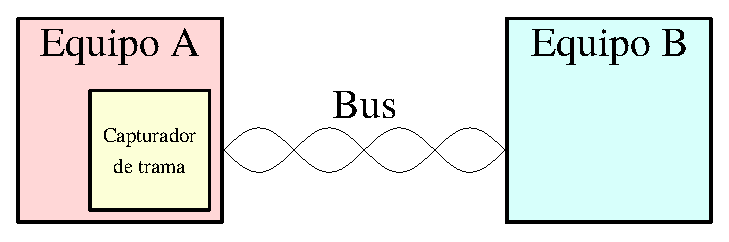
\includegraphics[width=80mm]{esquemas/esquema-captura-software.eps}
        \caption{Esquema de captura por medio de \textit{software}}
        \label{fig:captura-SW}
    \end{figure}
    
    \item \textbf{Utilizando un elemento \textit{hardware} intermedio entre los equipos (Figura~\ref{fig:captura-HW}).} \\
    Método que permite un mayor control y compatibilidad al ser totalmente independiente a los equipos implicados, pero que debido al uso de herramientas externas y a la necesidad de utilizar un equipo extra donde grabar y procesar los datos obtenidos, hace que sea un método mas laborioso, y por lo general, mas costoso.
    Se obtiene una mayor cantidad de información comparado al método \textit{software} al tener un acceso directo al propio bus.
    \begin{figure}[hbt]
        \centering
        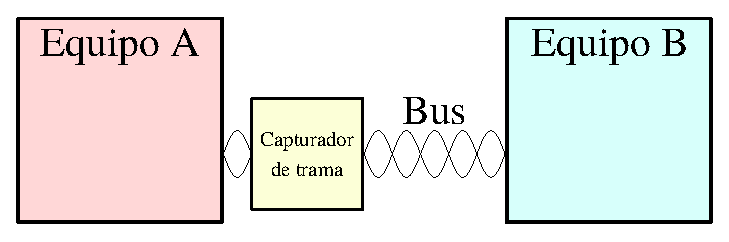
\includegraphics[width=80mm]{esquemas/esquema-captura-hardware.eps}
        \caption{Esquema de captura por medio de \textit{hardware}}
        \label{fig:captura-HW}
    \end{figure}
\end{enumerate}



\section{Sistemas \emph{software} actuales}
%* Comprobar
Debido a la gran facilidad y bajo coste que trae consigo el utilizar sistemas de captación \emph{software}, no es de extrañar que la gran mayoría de productos comerciales ya existentes se encuentran dentro de este grupo.

%* Comprobar
A continuación se muestra una lista detallada de los sistemas de captación \emph{software} más relevantes, clasificados según su tipo de licencia y ordenados según la fecha de última actualización.

%* Comprobar
\subsection{Licencia de tipo \emph{shareware}}
Se trata de \emph{software} no gratuito, de código cerrado y libre distribución entre usuarios\cite{hui2008economics}, que por lo general, posee un periodo de prueba en el que disfrutar la mayoría de las funciones sin coste. \\
Todos las aplicaciones descritas a continuación poseen una interfaz gráfica e intuitiva (Figura~\ref{fig:matriz-gui-close-sw}), y funcionan unicamente bajo al sistema operativo \emph{Windows\texttrademark}.

\begin{itemize}
    %* Comprobar
    \item \textbf{\emph{USB Monitor}\footnote{Página web del producto: \url{https://www.hhdsoftware.com/usb-monitor}} de \emph{HHD Software Ltd}.} \\
    Posee un periodo de prueba de 14 días en el que se permite utilizar todas las funciones sin restricciones. Su fecha de última actualización data del 15 de abril del 2019.

    Cabe destacar que este sistema tiene cuatro ediciones\footnote{Comparación completa de las ediciones de pago: \url{https://www.hhdsoftware.com/usb-monitor/compare}}, comentadas a continuación.
    \begin{enumerate}
        \item \textbf{Edición \emph{standard}.} \\ 
        Es la versión más básica. Incluye las siguientes funciones:
        \begin{itemize}
            \item Soporte para todas las versiones de USB.
            \item Funciones básicas de monitorización y visualizado.
            \item Filtros básicos.
            \item Guardado básico.
            \item Estadísticas de uso.
            \item Monitorización remota.
        \end{itemize}
        Su precio, a 27 de Marzo de 2019, es de 54.99\texteuro ~para uso NO comercial y 74.99\texteuro ~para uso comercial.

        \item \textbf{Edición gratuita\footnote{Se distribuye bajo el nombre de \emph{Free USB Analyzer} en: \url{https://freeusbanalyzer.com/}}.} \\
        Permite las mismas funciones que la edición \emph{standard}, limitando su uso máximo a cinco sesiones diarias, cada una de 10 minutos.
        
        \item \textbf{Edición \emph{professional}.} \\
        Incluye las ventajas de la edición \emph{standard}, añadiendo:
        \begin{itemize}
            \item Conversión de datos y visionado de datos \emph{HID}, imagen o audio, entre otros.
            \item Filtros en la captura.
            \item Capacidad de exportar los datos capturados de forma avanzada.
        \end{itemize}
        Su precio, a 27 de Marzo de 2019, es de 119.99\texteuro ~para uso NO comercial y 169.99\texteuro ~para uso comercial.
        
        \item \textbf{Edición \emph{ultimate}.} \\
        Incluye las ventajas de la edición \emph{professional}, añadiendo:
        \begin{itemize}
            \item Visor de paquetes USB en bruto.
            \item Monitorización simultanea de varios dispositivos.
            \item Scripts personalizados usando el lenguaje \emph{TypeSpript}.
        \end{itemize}
        Su precio, a 27 de Marzo de 2019, es de 159.99\texteuro ~para uso NO comercial y 224.99\texteuro ~para uso comercial.
    \end{enumerate}

    %* Comprobar
    \item \textbf{\emph{USB Sniffer}\footnote{Página web del producto: \url{https://www.eltima.com/products/usb-sniffer/}} de \emph{Eltima Software}.} \\
    \emph{Software} con 14 días de prueba, cuya versión completa tiene un precio único de mercado, a 27 de Marzo de 2019, de \$69.95 (sin incluir comisiones de cambio de divisa e impuestos). Su fecha de última actualización data del 15 de marzo del 2019.
    
    Hay que destacar las siguientes características\footnote{Lista completa de funciones: \url{https://www.eltima.com/products/usb-port-monitor\#tableCheckList}}.

    \begin{itemize}
        \item Vista completa y detallada de los datos entrantes y salientes.
        \item Soporte para \emph{HUBs} USB.
        \item Control de la captura según los datos de entrada.
        \item Soporte para todas las versiones de USB.
        \item Guardado avanzado de la trama capturada.
        \item Capacidad de marcar datos en la interfaz.
        \item Monitorización simultanea de varios dispositivos.
    \end{itemize}

    %* Comprobar
    \item \textbf{\emph{USBlyzer}\footnote{Página web del producto: \url{http://www.usblyzer.com/}}.} \\
    De manera similar que en los casos anteriores, brinda 33 días en los que probar todas la funcionalidades que ofrece sin ningún tipo de restricción. Su fecha de última actualización data del 15 de mayo del 2016.

    Caben destacar las siguientes características.

    \begin{itemize}
        \item Vista avanzada jerarquizada de todos los USB disponibles.
        \item Análisis de actividad del bus.
        \item Filtrado avanzado cuando se realizan búsquedas o capturas.
        \item Decodificación de una gran variedad de tipos de datos.
        \item Exportación avanzada.
    \end{itemize}
    El precio de una licencia, a 27 de Marzo de 2019, es de \$200 (sin incluir comisiones de cambio de divisa e impuestos), con descuentos de hasta un 46\% si se adquieren varias licencias.

    %* Comprobar
    \item \textbf{\emph{USBTrace}\footnote{Página web del producto: \url{http://www.sysnucleus.com/}} de \emph{SysNucleus}.} \\
    Igual que todos los anteriores, este programa utiliza una interfaz en la que mostrar y analizar en tiempo real el tráfico de puerto.

    Su periodo de prueba tiene una duración de 15 días, limitando además la cantidad total de la captura a 256Kb por sesión. Su fecha de última actualización data del 11 de noviembre del 2014.

    Entre otras\footnote{Lista de funciones completas: \url{http://www.sysnucleus.com/usbtrace_features.html}}, sus funciones más destacables son:
    \begin{itemize}
        \item Facilidad de uso y visualización.
        \item Variedad de filtros.
        \item Guardado avanzado.
        \item Permite análisis de los drivers utilizados por el equipo. 
        \item Captura en segundo plano.
        \item Decodificaciones personalizadas de los datos del bus.
    \end{itemize}
    Su precio unitario, a 27 de Marzo de 2019, asciende hasta \$125.00 (sin incluir comisiones de cambio de divisa e impuestos).
\end{itemize}

% \noWord[Quito las fotos??]
\begin{figure}[htbp]
    \centering
    \subfigure[\emph{USB Monitor} - \emph{HHD Software Ltd}]{
        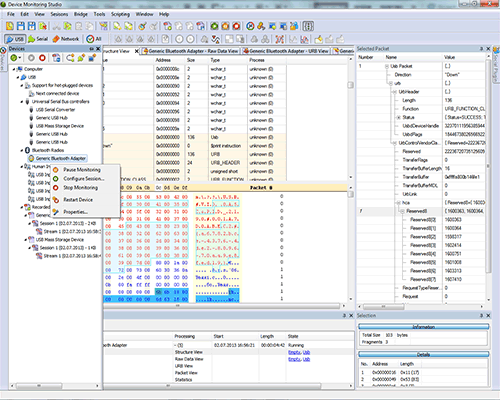
\includegraphics[width=67mm]{analizadores_software/HHD_Software-USB_Monitor.png}
        \label{fig:matriz-gui-close-sw:hdd}
    }
    \subfigure[\emph{USB Sniffer} - \emph{Eltima Software}]{
        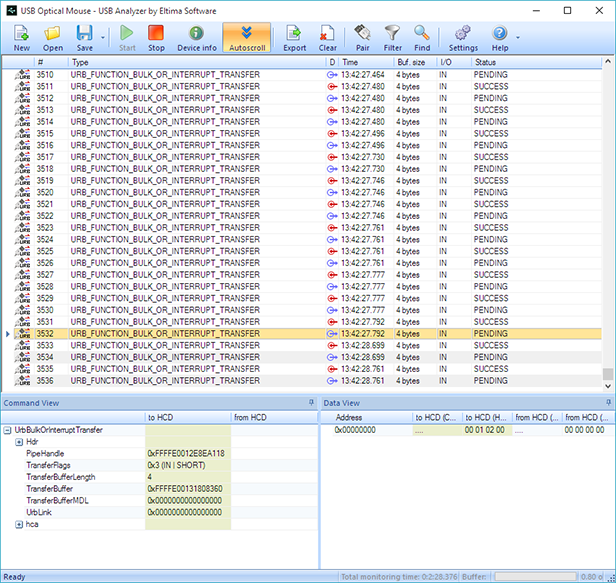
\includegraphics[width=67mm, height=55mm]{analizadores_software/eltima-USB_Sniffer.png}
        \label{fig:matriz-gui-close-sw:eltima}
    } \\
    \subfigure[\emph{USBlyzer}]{
        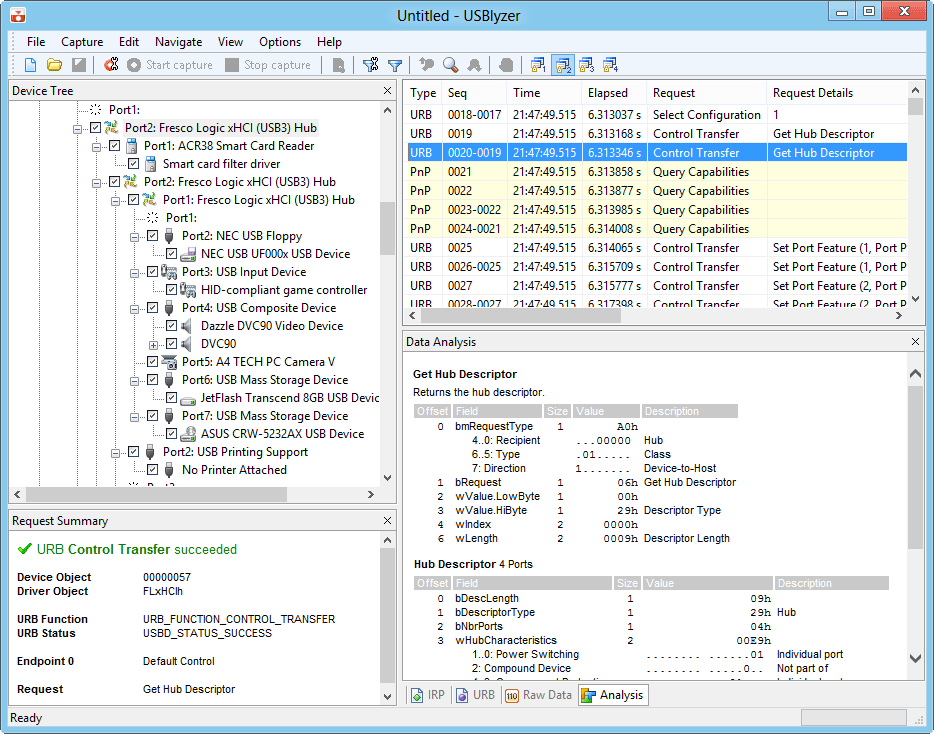
\includegraphics[width=67mm]{analizadores_software/usblyzer.png}
        \label{fig:matriz-gui-close-sw:usblyzer}
    }
    \subfigure[\emph{USBTrace} - \emph{SysNucleus}]{
        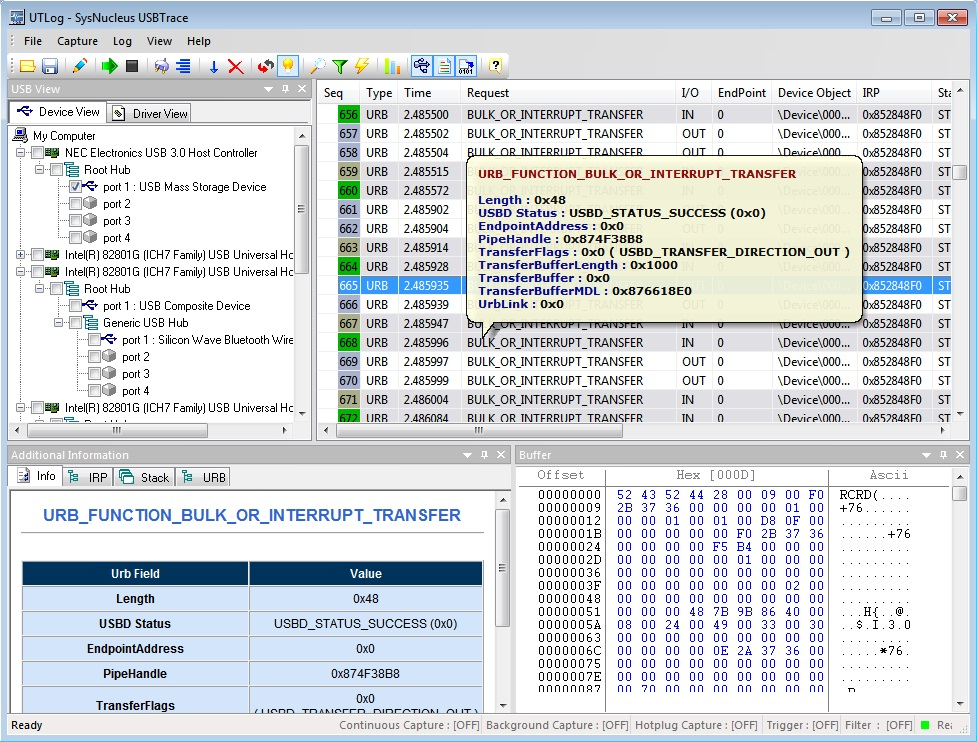
\includegraphics[width=67mm]{analizadores_software/SysNucleus-USBTrace.jpg}
        \label{fig:matriz-gui-close-sw:sysnucleus}
    }
    \caption{Interfaces gráficas de los analizadores \emph{software} de tipo \emph{shareware}. Imágenes extraídas de las páginas web de los desarrolladores.} 
    \label{fig:matriz-gui-close-sw}
\end{figure}


%* Comprobar
\subsection{Licencia de código libre}
Se trata de \emph{software} gratuito, cuyo código fuente está abiertamente disponible para su revisión y posibles modificaciones\cite{gonzalez2003introduccion}.

Dentro de este grupo hay que destacar dos herramientas, con funcionalidades similares, pero disponibles una bajo el sistema operativo \emph{Windows\texttrademark}, y la otra bajo sistemas \emph{UNIX-like}\footnote{Sistemas con comportamiento similar a sistemas Unix, sin ser necesariamente certificado a ninguna \emph{Single Unix Specification} (En español, Especificación Única Unix).}.

\begin{itemize}
    %* Comprobar
    \item \textbf{\emph{Tcpdump}\footnote{Página web del \emph{software}: \url{https://www.tcpdump.org/}}.} \\
    Herramienta bajo licencia BSD\footnote{Información detallada de la licencia: \url{https://www.tcpdump.org/license.html}}, que a través de una linea de comandos, es capaz de capturar, analizar y almacenar en un archivo PCAP paquetes de una amplia variedad de interfaces, entre las que se encuentra dispositivos \emph{USB}.

    Este método, debido a su especialización, no sería capaz de realizar un análisis detallado, por lo que sería necesario un programa adicional que posteriormente haga el estudio y clasificación de los datos de forma gráfica.

    Funciona en sistemas \emph{UNIX-like}, siempre que se tenga acceso la interfaz USB.
    
    %* Comprobar
    \item \textbf{\emph{USBPcap}\footnote{Página web del \emph{software}: \url{https://desowin.org/usbpcap/}}.} \\
    Realiza funciones similares a las que realiza \emph{Tcpdump} en cuanto a captura USB, pero funcionando bajo el Sistema Operativo Windows\texttrademark. Posee licencias GPLv2 y BSD.
    
    De igual manera que en el caso anterior, sigue siendo necesario el uso de \emph{software} de terceros para su análisis completo.
\end{itemize}

%* Comprobar
Dichos archivos generados, por lo general de tipo \emph{pcap}\cite{guyharris2015}, se pueden analizar a través de la herramienta gráfica de análisis de paquetes \emph{Wireshark}\footnote{Página web del \emph{software}: \url{https://www.wireshark.org/}} (véase figura~\ref{fig:gui-open-wireshark}). Esta está disponible para cualquiera de los dos sistemas operativos anteriores.

Hay destacar, que esta herramienta, y unicamente bajo sistemas basado en \emph{Linux}, puede ser capaz de capturar directamente y en tiempo real las tramas \emph{USB}.

\begin{figure}[hbt]
    \centering
    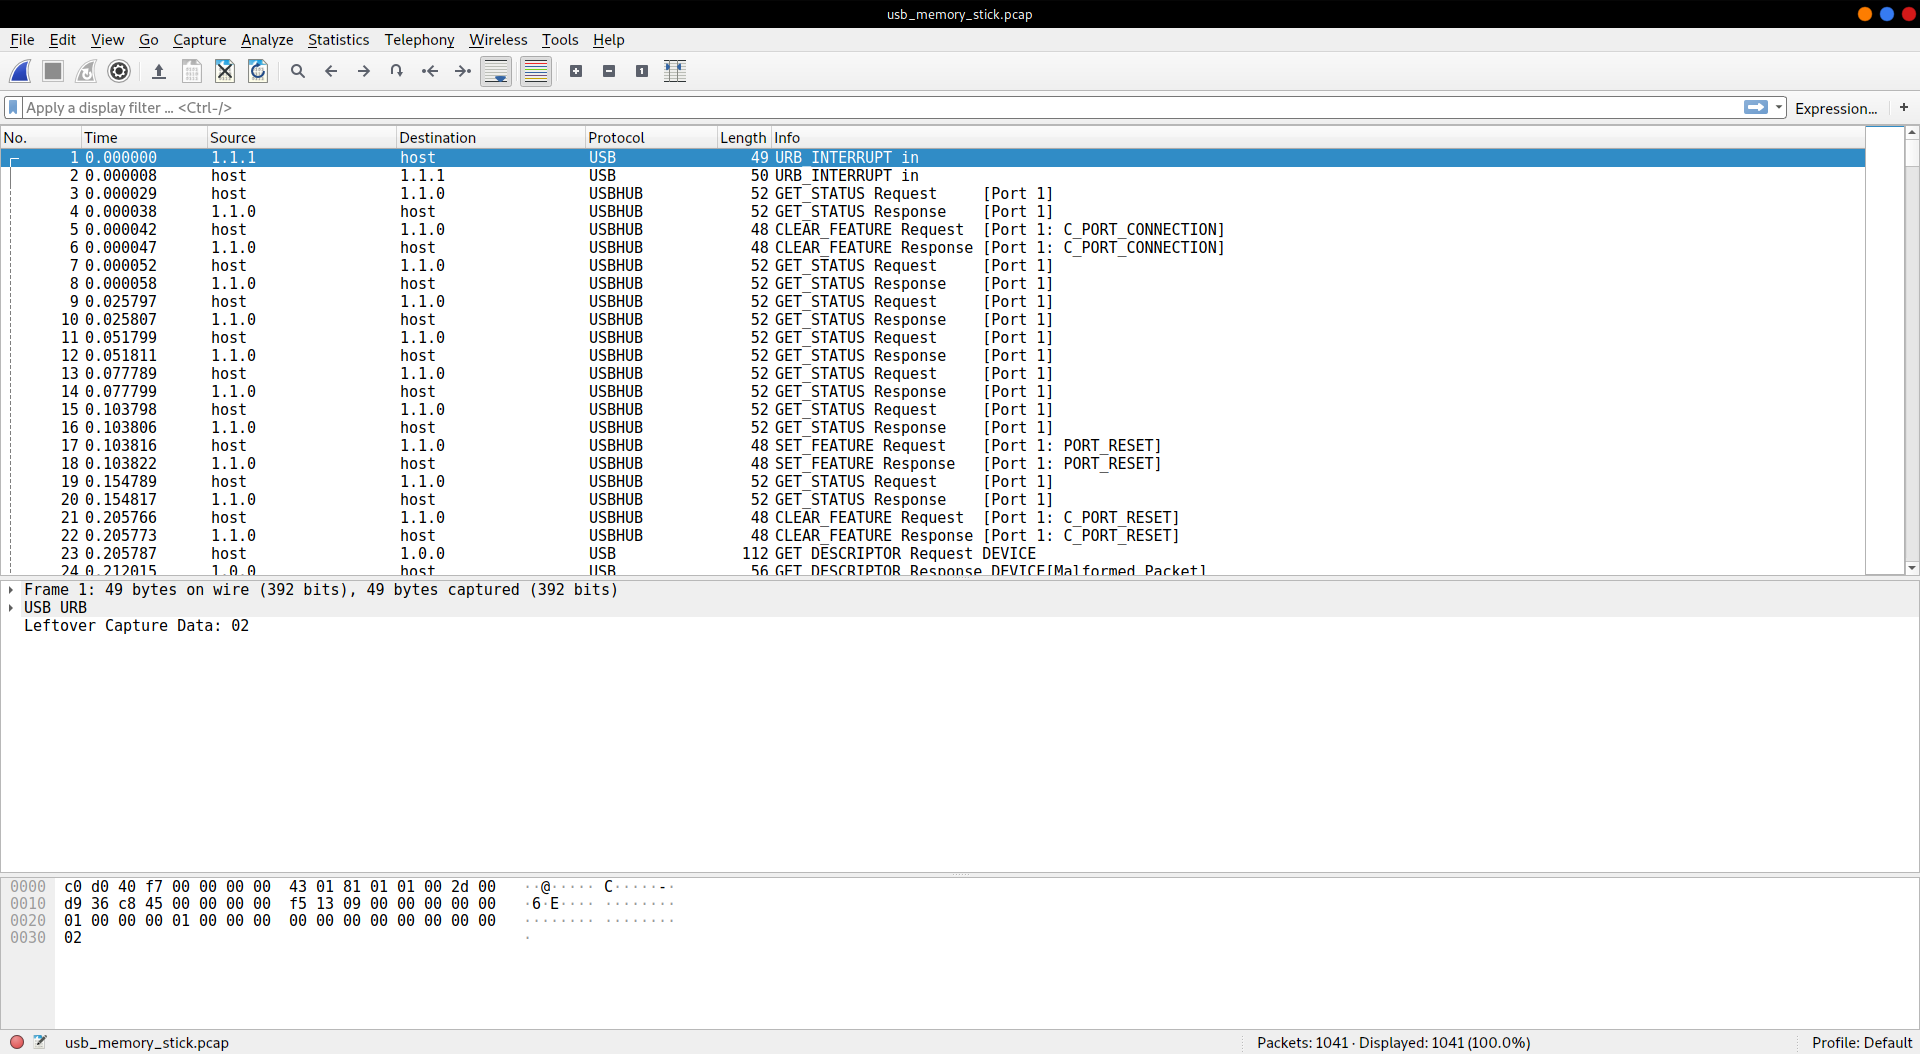
\includegraphics[width=125mm]{analizadores_software/wireshark.png}
    \caption{Interfaz gráfica del analizador de paquetes \emph{Wireshark}}
    \label{fig:gui-open-wireshark}
\end{figure}


%!
\section{Sistemas \emph{hardware} actuales}
En caso de que no sea posible la utilización de una captura por \emph{software}, ya sea por incompatibilidades, falta de acceso, necesidad de obtener más datos de interés o cualquier otra causa, se tendría que utilizar un sistema más complejo y costoso, por medio de \emph{hardware}.

%* Comprobar 
A continuación se muestran varios ejemplos ya existentes de este tipo, todos ellos soportan hasta la versión 2.0 de USB. \\

\textit{Nota. Todos los precios de la siguiente lista, excepto que se indique, no incluyen envío, impuestos locales, o tasas de cambio de divisa.}

\begin{itemize}
    %* Comprobar 
    \item \textbf{\emph{USB Explorer 200} de \emph{Ellisys}\footnote{Página web del producto: \url{https://www.ellisys.com/products/usbex200/index.php}}.}
    
    Sistema comercial, que entre otras características\cite{ellisys2008}, destacan:
    \begin{itemize}
        \item Soporte para USB 2.0 \emph{high speed} ($480~Mbit/s$), \emph{full speed} ($12~Mbit/s$) y \emph{low speed} ($1.5~Mbit/s$).
        \item \emph{Trigger} externo de hasta 5V de entrada o 3.3V de salida.
        \item Memoria interna FIFO de $32~MBytes$.
        \item Alimentación a través de la propia conexión USB en el equipo de análisis.
        \item Dimensiones aproximadas de 150x120x65mm con un peso de 750 gramos. Véase figura~\ref{fig:ellisys-Explorer200}.
    \end{itemize}

    Aun siendo el mismo producto, este está limitado, existiendo tres variaciones, cada una con más funcionalidades y mayor precio respecto a la anterior.

    \begin{enumerate}
        \item \textbf{Edición básica.} \\
        Es la versión más básica, permitiendo unicamente capturar y posteriormente almacenar en el equipo de análisis la trama USB. \\
        Su precio, a 27 de Marzo de 2019, es de 799\texteuro.
      
        \item \textbf{Edición estándar.} \\
        Incluye las ventajas de la edición básica, añadiendo:
        \begin{itemize}
            \item Captura en tiempo real.
            \item Filtros de captura.
            \item Resumen del tráfico existente.
            \item Decodificación parcial del protocolo USB.
        \end{itemize}
        Su precio, a 27 de Marzo de 2019, es de 1599\texteuro.
        
        \item \textbf{Edición profesional.} \\
        Incluye las ventajas de la edición estándar, añadiendo:
        \begin{itemize}
            \item Decodificación completa USB.
            \item Análisis del protocolo.
            \item Capacidad de usar disparos (\emph{triggers}) externos.
        \end{itemize}
        Su precio, a 27 de Marzo de 2019, es de 3199\texteuro.
    \end{enumerate}    
    \begin{figure}[htb]
        \centering
        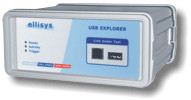
\includegraphics[width=50mm]{analizadores_hardware/ellisys_USBExplorer200.jpg}
        \caption{\emph{Ellisys USB Explorer 200}. Imagen extraída de la página web del fabricante.}
        \label{fig:ellisys-Explorer200}
    \end{figure}
    
    %* Comprobar
    \item \textbf{\emph{Mercury T2} de \emph{Teledyne LeCroy}\footnote{Página web del producto: \url{https://teledynelecroy.com/protocolanalyzer/usb/mercury-t2}}.}
    
    Sistema comercial, que entre otras características\cite{teledynelecroy2014}, destacan:
    \begin{itemize}
        \item Soporte para USB 2.0 \emph{high speed} ($480~Mbit/s$), \emph{full speed} ($12~Mbit/s$) y \emph{low speed} ($1.5~Mbit/s$).
        \item Memoria interna de $256~MBytes$.
        \item Almacenado automática en disco para permitir capturas de larga duración.
        \item \emph{Trigger} externo (necesario adaptador externo no incluido).
        \item Alimentación a través de la propia conexión USB en el equipo de análisis.
        \item Dimensiones aproximadas de 80x90x24mm con un peso de 158 gramos. Véase figura~\ref{fig:TeledyneLeCroy-MercuryT2}.
    \end{itemize}
    
    De igual manera que en el producto anterior, este posee varias versiones.

    \begin{enumerate}
        \item \textbf{Edición estándar.} \\
        Incluye las siguientes opciones:
        \begin{itemize}
            \item Captura y almacenaje de cualquier trama USB hasta 2.0 en tiempo real.
            \item Disparos (\emph{triggers}) para almacenar captura tanto externos, como detectando patrones en la trama.
        \end{itemize}
        Su precio, a 27 de Marzo de 2019, es de \$901.
        
        \item \textbf{Edición avanzada.} \\
        Incluye las ventajas de la edición estándar, añadiendo:
        \begin{itemize}
            \item Estadísticas en tiempo real del bus.
            \item Exportación en formato .csv.
            \item API de automatización.
        \end{itemize}
        Su precio, a 27 de Marzo de 2019, es de \$1235.
    \end{enumerate}
    \begin{figure}[htb]
        \centering
        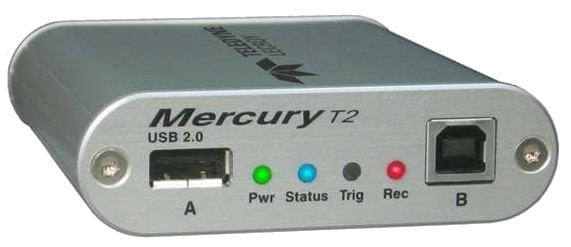
\includegraphics[width=50mm]{analizadores_hardware/TeledyneLeCroy_MercuryT2.jpg}
        \caption{\emph{Teledyne LeCroy Mercury T2}. Imagen extraída de la página web del fabricante.}
        \label{fig:TeledyneLeCroy-MercuryT2}
    \end{figure}

    %* Comprobar
    \item \textbf{\emph{Beagle USB} de \emph{Total Phase}\footnote{Página web del producto: \url{https://www.totalphase.com/protocols/usb/}}.}
    
    Dentro de la amplia gama de productos que disponen, hay dos que destacan principalmente.
    \begin{enumerate}
        \item \textbf{\emph{Beagle USB 480}\cite{totalphase12-2018}.}
        De todas las versiones que poseen, esta es la más básica que permite hasta capturas \emph{high speed} de ($480~Mbit/s$).
        \begin{itemize}
            \item Captura en tiempo real.
            \item Estadísticas en tiempo real.
            \item $64MBytes$ de memoria integrada.
            \item \emph{Triggers} externos de entrada y salida.
            \item Sincronización básica.
            \item API de control.
        \end{itemize}
        Su precio, a 27 de Marzo de 2019, es de \$2250.
        
        \item \textbf{\emph{Beagle USB 480 Power}\cite{totalphase480-2018} - Edición estándar.} \\
        Posee las mismas ventajas que el producto anterior, pero aumentando la memoria integrada de $64MBytes$ a $256MBytes$ y añadiendo capacidad de medir la tensión y corriente del propio Bus.\\
        Su precio, a 27 de Marzo de 2019, es de \$1599.
        
        \item \textbf{\emph{Beagle USB 480 Power}\cite{totalphase480-2018} - Edición \emph{ultimate}.} \\
        Mejora las capacidades de disparos (\emph{triggers}) respecto a la versión estándar.\\
        Su precio, a 27 de Marzo de 2019, es de \$2950.
    
        \begin{figure}[htbp]
            \centering
            \subfigure[\emph{Beagle USB 480}]
            {
                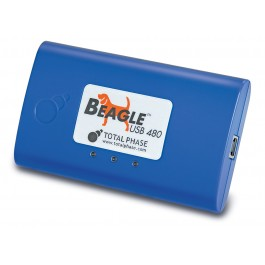
\includegraphics[width=40mm]{analizadores_hardware/TotalPhase_beagle480.jpg}
                \label{fig:TotalPhase-480}
            }
            \subfigure[\emph{Beagle USB 480 Power}]{
                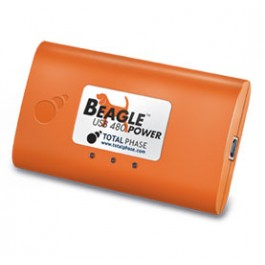
\includegraphics[width=40mm]{analizadores_hardware/TotalPhase_beagle480Power.jpg}
                \label{fig:TotalPhase-480Power}
                }
            \caption{Productos de \emph{Total Phase}. Imágenes extraídas de la página web del fabricante.} 
            \label{fig:TotalPhase}
        \end{figure}
    \end{enumerate}
    
    %* Comprobar
    \item \textbf{\emph{USB Sniffer}\footnote{Página web del proyecto: \url{http://ultra-embedded.com/usb_sniffer/}} de \emph{Ultra-Embedded}}

    Proyecto NO comercial, que usando una \emph{FPGA Xilinx Spartan 6 LX9}, y una placa de desarrollo encargada de procesar la capa física, es capaz de capturar hasta USB 2.0 \emph{high speed} ($480~Mbit/s$). En la figura~\ref{fig:ultra-embedded} se muestra una imagen del proyecto.
    
    Al ser un proyecto personal, no dispone de un producto final que se pueda adquirir, por lo que si se quiere utilizar se deben comprar las piezas por separado. Además, el código utilizado es \emph{open source}, por lo que se puede replicar sin ningún tipo de problema. Su precio aproximado se muestra en la tabla~\ref{tab:precio-ultra-embedded}.

    \begin{table}[hbtp]
        \centering
        \caption{Componentes y precio de la propuesta de analizador USB de \emph{Ultra-Embedded}}
        \label{tab:precio-ultra-embedded}
        \begin{tabular}{|c|c|c|}
            \hline
            \textbf{Componente} &
            \textbf{Unidades} &
            \textbf{Precio} \\ \hline
            \hline

            FPGA Xilinx Spartan 6 LX9 &
            1 & \$75 \\ \hline

            Placa de desarrollo USB3300 &
            1 &
            \$8 \\ \hline

            Cable IDC &
            1 &
            \$5 \\ \hline

            \multicolumn{1}{l}{} &
            \multicolumn{1}{l}{} &
            \multicolumn{1}{l}{} \\

            \multicolumn{2}{r}{Precio total:} &
            \multicolumn{1}{l}{\$88} \\
        \end{tabular}
    \end{table}

    \begin{figure}[hbtp]
        \centering
        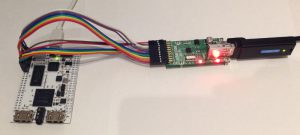
\includegraphics[width=85mm]{analizadores_hardware/Ultra-Embedded.jpg}
        \caption{\emph{USB Sniffer}. Imagen extraída de la página web del proyecto.}
        \label{fig:ultra-embedded}
    \end{figure}
\end{itemize}



%* Comprobar
\section{Comparativa de sistemas}
%* Comprobar
En la tabla~\ref{tab:comparacion-sw} se muestra una comparativa de los productos de captura \emph{software} más destacados.

Se aprecia, que dentro del \emph{software} de pago, el que más funcionalidades ofrece a razón de su precio, es \emph{USB Sniffer} de \emph{Eltima Software}, seguido de \emph{USB Monitor} de \emph{HHD Software Ltd}. Las otras dos opciones no poseen actualizaciones recientes, y su precio es más elevado, por lo que son menos recomendables.

Por otro lado, las opciones de \emph{código libre}, aun teniendo una curva de aprendizaje muy superior, son opciones totalmente viables y recomendables.

%* Comprobar
\begin{table}[hbtp]
    \centering
    \caption{Comparativa de sistemas \emph{software}}
    \label{tab:comparacion-sw}
    \begin{tabular}{|c|c|c|c|c|}
        \hline
        Nombre &
        \begin{tabular} {@{}c@{}}
            Licencia y \\ precio
        \end{tabular} &
        Ventajas &
        Desventajas \\ \hline
        \hline
        
        \begin{tabular}
            {@{}c@{}} \textbf{\emph{USB Monitor}} de \\ \emph{HHD Software Ltd}
        \end{tabular} &
        \begin{tabular} {@{}c@{}}
            \emph{Shareware} \\ Desde 54.99\texteuro
        \end{tabular} &
        \begin{tabular} {@{}c@{}}
            Actualizaciones frecuentes. \\
            Decodificación \enquote{en vivo}. \\
            Gran sencillez de uso. \\
            Posee versión gratuita. \\
        \end{tabular} &
        \begin{tabular} {@{}c@{}}
            Extra para uso comercial.  \\
            Varias ediciones. \\
        \end{tabular} \\ \hline
        
        \begin{tabular}
            {@{}c@{}} \textbf{\emph{USB Sniffer}} de \\ \emph{Eltima Software}
        \end{tabular} &
        \begin{tabular} {@{}c@{}}
            \emph{Shareware} \\ \$69.95
        \end{tabular} &
        \begin{tabular} {@{}c@{}}
            Monitorización simultanea. \\
            Soporte para \emph{HUBs} USB. \\
            Gran sencillez de uso. \\
        \end{tabular} &
        \begin{tabular} {@{}c@{}}
            Sin capacidad de decodificación. \\
        \end{tabular} \\ \hline
        
        \textbf{\emph{USBlyzer}} &
        \begin{tabular} {@{}c@{}}
            \emph{Shareware} \\ Hasta \$200
        \end{tabular} &
        \begin{tabular} {@{}c@{}}
            Decodificación incluida. \\
            Exportación avanzada.  \\
        \end{tabular} &
        \begin{tabular} {@{}c@{}}
            Sin actualizaciones recientes. \\
            Precio elevado. \\
        \end{tabular} \\ \hline
        
        \begin{tabular}
            {@{}c@{}} \textbf{\emph{USBTrace}} de \\ \emph{SysNucleus}
        \end{tabular} &
        \begin{tabular} {@{}c@{}}
            \emph{Shareware} \\ \$125.00
        \end{tabular} &
        \begin{tabular} {@{}c@{}}
            Decodificado personalizado. \\
            Análisis de \emph{drivers}. \\
        \end{tabular} &
        \begin{tabular} {@{}c@{}}
            Sin actualizaciones recientes. \\
            Pocas funcionalidades. \\
        \end{tabular} \\ \hline
        
        \begin{tabular}
            {@{}c@{}} \textbf{\emph{Tcpdump}} y \\ \textbf{\emph{USBPcap}}
        \end{tabular} &
        \begin{tabular} {@{}c@{}}
            \emph{Código libre} \\ --
        \end{tabular} &
        \begin{tabular} {@{}c@{}}
            Soporte de la comunidad. \\
            Multiplataforma. \\
            Gratuito. \\
        \end{tabular} &
        \begin{tabular} {@{}c@{}}
            Solo realiza capturas de trama. \\
            Pocas funcionalidades extra. \\
            Sin interfaz gráfica. \\
        \end{tabular} \\ \hline
        
        \textbf{\emph{Wireshark}} &
        \begin{tabular} {@{}c@{}}
            \emph{Código libre} \\ --
        \end{tabular} &
        \begin{tabular} {@{}c@{}}
            Variedad de funcionalidades. \\
            Filtrado avanzado. \\
            Multiplataforma. \\
            Gratuito. \\
        \end{tabular} &
        \begin{tabular} {@{}c@{}}
            No realiza capturas. \\
            Poco intuitivo. \\
        \end{tabular} \\ \hline
    \end{tabular}
\end{table}

%* Comprobar
En la tabla~\ref{tab:comparacion-hw} se muestra una comparativa de los productos de captura \emph{hardware} más destacados.

Se aprecia que dentro de este grupo, el equipo más recomendable a razón de sun funcionalidades ofrecidas y precio es el \emph{Mercury T2} de \emph{Teledyne LeCroy}. Si se buscan más funciones y almacenamiento es más viable utilizar el  {\emph{Beagle USB 480 Power} de \emph{Total Phase}.

%* Comprobar
\begin{table}[hbtp]
    \centering
    \caption{Comparativa de sistemas \emph{hardware}}
    \label{tab:comparacion-hw}
    \begin{tabular}{|c|c|c|c|c|}
        \hline
        Nombre &
        \begin{tabular} {@{}c@{}}
            Licencia y \\ precio
        \end{tabular} &
        Ventajas &
        Desventajas \\ \hline
        \hline
        
        \begin{tabular}
            {@{}c@{}} \textbf{\emph{USB Explorer 200}} de \\ \emph{Ellisys}
        \end{tabular} &
        \begin{tabular} {@{}c@{}}
            Cerrado. \\ Desde 799\texteuro \\ a 3199\texteuro
        \end{tabular} &
        \begin{tabular} {@{}c@{}}
            Posibilidad de análisis completo. \\
            Captura en tiempo real. \\
            Disparos externos. \\
        \end{tabular} &
        \begin{tabular} {@{}c@{}}
            Versión básica simple. \\
            Escasa memoria. \\
            Sistema costoso. \\
        \end{tabular} \\ \hline
        
        \begin{tabular}
            {@{}c@{}} \textbf{\emph{Mercury T2}} de \\ \emph{Teledyne LeCroy}
        \end{tabular} &
        \begin{tabular} {@{}c@{}}
            Cerrado. \\ Desde \$901 \\ a \$1235
        \end{tabular} &
        \begin{tabular} {@{}c@{}}
            API de automatización. \\
            Disparos avanzados. \\
            Tamaño reducido. \\
        \end{tabular} &
        \begin{tabular} {@{}c@{}}
            Adaptador para disparos \\ externos no incluido. \\
            Pocas funciones extras. \\
        \end{tabular} \\ \hline
        
        \begin{tabular}
            {@{}c@{}} \textbf{\emph{Beagle USB 480}} de \\ \emph{Total Phase}
        \end{tabular} &
        \begin{tabular} {@{}c@{}}
            Cerrado. \\ \$2250
        \end{tabular} &
        \begin{tabular} {@{}c@{}}
            Estadisticas en tiempor real. \\
            API de automatización. \\
            Sincronización básica. \\
        \end{tabular} &
        \begin{tabular} {@{}c@{}}
            Sin funciones de analisis. \\
            Escasa memoria. \\
        \end{tabular} \\ \hline
        
        \begin{tabular}
            {@{}c@{}} \textbf{\emph{Beagle USB 480 Power}} de \\ \emph{Total Phase}
        \end{tabular} &
        \begin{tabular} {@{}c@{}}
            Cerrado. \\ Desde \$1599 \\ a \$2950
        \end{tabular} &
        \begin{tabular} {@{}c@{}}
            Alta capacidad de memoria. \\
            Analisis de potencia. \\
        \end{tabular} &
        \begin{tabular} {@{}c@{}}
            Versión estándar sin \\disparos avanzados. \\
        \end{tabular} \\ \hline
        
        \begin{tabular}
            {@{}c@{}} \textbf{\emph{USB Sniffer}} de \\ \emph{Ultra-Embedded}
        \end{tabular} &
        \begin{tabular} {@{}c@{}}
            Código libre. \\ Aporx. \$88
        \end{tabular} &
        \begin{tabular} {@{}c@{}}
            Muy económico. \\
            Código libre. \\
        \end{tabular} &
        \begin{tabular} {@{}c@{}}
            No está en venta directa. \\
            Solo permite captura. \\
            Memoria escasa. \\
        \end{tabular} \\ \hline
    \end{tabular}
\end{table}



% \chapter{Motivación y antecedentes}
% \label{ch:antecedentes_plantilla}

% El problema que pretendes resolver está dentro de un contexto que el cliente debe conocer.  Esta sección aporta información para conocer en detalle la importancia del problema y la dificultad para resolverlo con los productos y programas disponibles actualmente.

% Este capítulo concentrará el grueso de las citas del TFG.  Dado que se trata del primer trabajo profesional, el alumno no suele estar familiarizado con las citas bibliográficas.  Pon toda tu atención en qué citas y cómo lo citas.  Revisa la sección~\ref{sec:bibliografia-citas} para las reglas mínimas que deben cumplir las citas.

% \warning{Es muy importante respetar la regla de atribuir correctamente.  No es aceptable desde el punto de vista legal, ni tampoco desde el punto de vista ético, copiar trabajo de otros sin atribuirlo correctamente a los autores.}

% Esta sección debe estudiar de forma sistemática todas las opciones ya disponibles en la actualidad para resolver el problema. No basta con una mera enumeración, hay que estudiarlos mínimamente para explicar por qué no son una solución para el problema o qué podría aportar a la solución del problema.

% Un método sistemático para realizar esta parte del TFG es la revisión sistemática de literatura, conocida habitualmente por sus siglas en inglés SLR (\emph{Sistematic Literature Review}).  Un resumen muy sencillo de cómo realizar una SLR puede encontrarse en~\cite{anderskofodpetersen2014}.  También encontrarás consejos prácticos en~\cite{sandroschulze2017}.  Para un proceso más detallado, especialmente si tu problema tiene mucho arte previo, puedes consultar~\cite{barbarakitchenhamstuartcharters2007}.  Si no hay mucho arte previo pon este capítulo y el siguiente juntos.

% En una tesis doctoral el análisis sistemático del estado del arte es esencial. En un TFG es importante, pero no hay que perder la cabeza.  Un TFG son unas 300 horas de trabajo de un estudiante medio que ya posea los conocimientos generales necesarios (volveremos a esto más tarde).  Considero que un buen análisis del estado del arte corresponde a un trabajo de entre 25 horas y 100 horas, dependiendo del tema del proyecto.  Si el tema es muy específico es más fácil hacer el estudio del estado del arte.

% Termina este capítulo con una sección que resuma el estado del arte e identifique las lagunas lo más claramente posible.  Una tabla comparativa o un gráfico pueden ser formas interesantes de presentar la información. %* Comprobar [4/06 - 4/06]
\chapter{Objetivos}
\label{ch:objetivos}

%* Comprobar
Bajo la premisa de realizar un \textbf{analizador USB \emph{hardware} de bajo coste} con herramientas y utilidades de código libre, el presente Trabajo Fin de Grado se ha descompuesto en varios objetivos parciales, estos siguen siempre una metodología SMART, es decir, deben ser Simples, Medibles, Acordados, Realista y Temporizados.

%* Comprobar
\section{Selección de componentes \emph{hardware}}
Debido a la flexibilidad que supone utilizar una FPGA\cite{monmasson2007fpga}, se propone diseñar el sistema de captura a partir de una. Por otra parte, ya que existen circuitos especializados en procesar capas física USB, es de gran interés incluir uno de ellos\footnote{La idea de utilizar un integrado especializado, se obtiene del sistema \emph{USB Sniffer} planteado por \emph{Ultra-Embedded}, nombrado en el capitulo~\ref{ch:antecedentes} de antecedentes.}, pudiendo abstraer de esa forma ciertas partes de la comunicación USB de poco interés, y reduciendo en cierta medidas posibles errores de sincronización.

Se deben buscar por tanto, todos aquellos componentes necesarios, de la forma más económica posible, para elaborar el sistema de captura. Seguidamente, se ha de elegir como se conexionan mutuamente.

%* Comprobar
\section{Implementación de memoria \emph{FIFO}}
Diseño e implementación de un módulo en lenguaje Verilog que actúe como memoria \emph{FIFO}. Este será capaz de almacenar información de tal manera que el primer $bit$ introducido sea el primero en ser recuperado.

Dado que la FPGA a utilizar dispone de varios bloques de RAM específicos, se utilizarán varios de estos para no depender unicamente de registros, consiguiendo una mayor capacidad de almacenamiento, con un circuito lo mayor optimizado posible.

La gran mayoría los módulos a diseñar dependen en gran medida de este tipo de memoria, por lo que es esencial disponer de ella en el la mayor brevedad posible, a su vez, y debido a su gran utilidad, la velocidad\cite{rose1993architecture} máxima a la que puede funcionar el sistema en su conjunto está dada por su velocidad de escritura/lectura de datos.

En la figura~\ref{fig:FIFO_info} se muestra un esquema del resultado esperado.

\begin{figure}[htb]
    \centering
    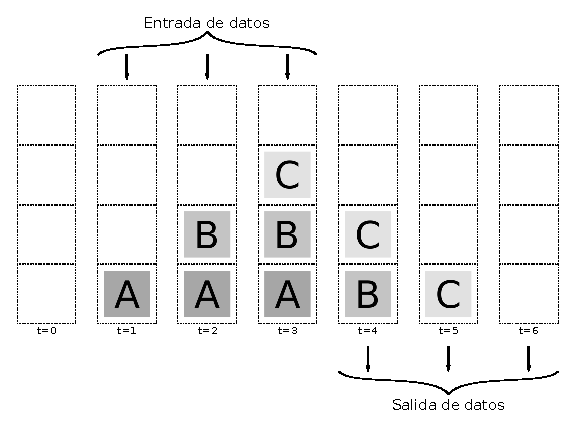
\includegraphics[width=80mm]{esquemas/FIFO_bw.eps}
    \caption{Esquema de funcionamiento de una memoria \emph{FIFO}.}
    \label{fig:FIFO_info}
\end{figure}



%* Comprobar
\section{Implementación de un sistema de comunicación serie}
Diseño e implementación de un sistema en lenguaje Verilog que sea capaz de comunicarse bidireccionalmente usando un puerto serie simple\cite{design-uart-vhdl}, pudiendo conectarse a él por medio del circuito integrado FTDI FT2232HL\footnote{Circuito encargado de convertir una conexión \emph{USB High Speed} a dos protocolos configurables distintos. En el caso de la placa de desarrollo \emph{IceStick}, se utiliza un canal para programar la memoria \emph{Flash} SPI utilizada por la FPGA, y otro para proporcionar una comunicación UART hacia el equipo.} (disponible en la placa de desarrollo \emph{IceStick}\cite{icestickmanual}), o utilizando un equipo externo compatible.

Por dicho puerto, la FPGA transmitirá tanto la trama USB capturada como información del bus, y recibirá los comandos que debe seguir.

En la figura~\ref{fig:serie_esquema} se muestra una señal típica serie, esta es la señal que debe ser capturada y generada en la FPGA.

\begin{figure}[htb]
    \centering
    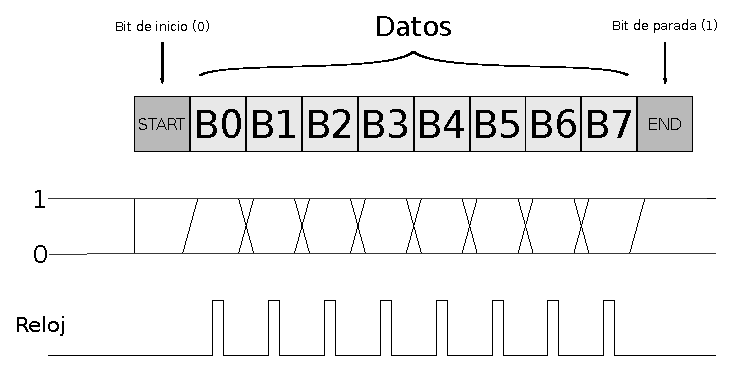
\includegraphics[height=52mm]{esquemas/serie.eps}
    \caption{Señal típica de una comunicación serie.}
    \label{fig:serie_esquema}
\end{figure}

A su vez, este objetivo se puede descomponer en varios subobjetivos.

%* Comprobar
\subsection{Diseño de un módulo de emisión serie}
Módulo capaz de controlar los datos almacenados en una memoria \emph{FIFO}, para posteriormente transmitirlos por el puerto serie.

%* Comprobar
\subsection{Diseño de un módulo de recepción serie}
Módulo capaz almacenar en una memoria \emph{FIFO} los datos paralelizados capturados en el puerto serie.



%* Comprobar
\section{Implementación de un sistema que procese el protocolo ULPI}
Diseño e implementación de un sistema en lenguaje Verilog capaz de comunicarse con otros dispositivos compatibles con el protocolo ULPI (\emph{UTMI+ Low Pin Interface}), siendo en este caso, el integrado USB3300 de \emph{Microchip}, encargado de la capa física USB.

Todas las características y casos del protocolo ULPI están completamente definidas tanto en la hoja de especificaciones del propio protocolo\cite{ulpi-specs} como en la hoja de características del circuito integrado USB3300\cite{microchip:usb3300}. Hay que destacar que el bus consta de una señal de reloj a $60MHz$ a la que se referencia el resto de señales (\emph{CLK}), 8 señales de datos bidireccionales paralelos (\emph{DATA}), una señal de control de dirección (\emph{DIR}) y dos señales extra de control (\emph{STP} y \emph{NXT}).

Puesto que unicamente queremos obtener de forma pasiva los datos USB, de los cuatro posibles modos de funcionamiento ULPI, escritura de registros, lectura de registros, recepción de datos USB y envío de datos USB, solo es interesante diseñar los tres primeros, por lo que este objetivo se puede dividir en las siguientes partes.

%* Comprobar
\subsection{Diseño de un módulo de escritura de registros ULPI}
Módulo capaz de generar y procesar las señales ULPI necesarias para almacenar un valor arbitrario de $8~bits$, en un registro del integrado conectado por ULPI.

En la figura~\ref{fig:ULPI_REG_WRITE} se puede apreciar la comunicación básica usada para realizar dicha escritura.
\begin{figure}[hbt]
    \centering
    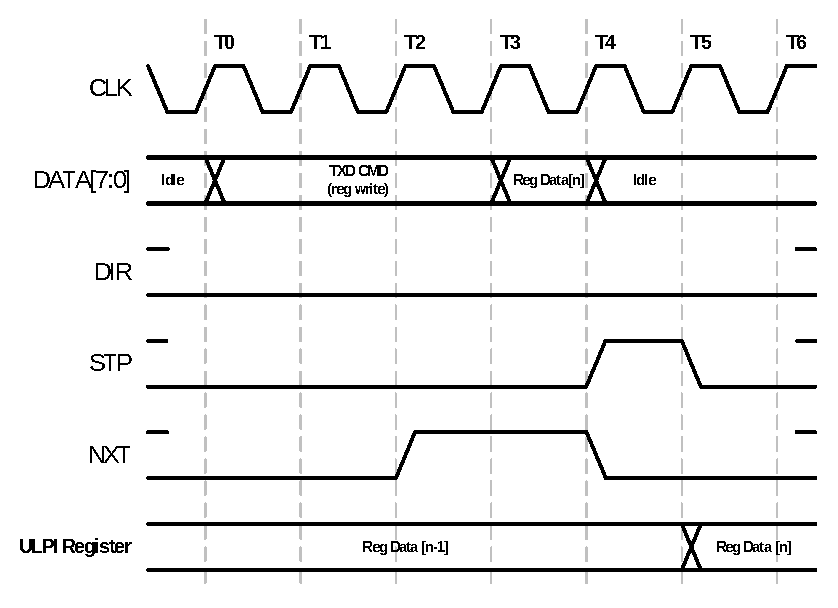
\includegraphics[width=90mm]{datasheets/USB3300_REG_WRITE.eps}
    \caption{Trama de escritura de registros ULPI.}
    \label{fig:ULPI_REG_WRITE}
\end{figure}

%* Comprobar
\subsection{Diseño de un módulo de lectura de registros ULPI}
Módulo capaz de generar y procesar las señales ULPI necesarias para obtener un valor almacenado en un registro arbitrario del integrado conectado por ULPI.

En la figura~\ref{fig:ULPI_REG_READ} se puede apreciar la comunicación básica usada para realizar dicha lectura.
\begin{figure}[hbt]
    \centering
    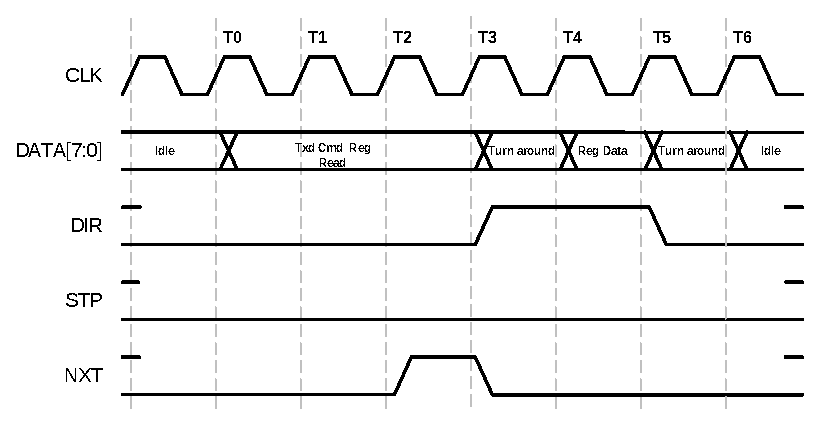
\includegraphics[width=90mm]{datasheets/USB3300_REG_READ.eps}
    \caption{Trama de lectura de registros ULPI.}
    \label{fig:ULPI_REG_READ}
\end{figure}

%* Comprobar
\subsection{Diseño de un módulo de captación USB}
Módulo que ante la llegada de datos USB, sea capaz de procesar las señales ULPI para obtener y clasificar la trama transmitida. En la figura~\ref{fig:ULPI_RECV} se puede apreciar la comunicación básica existente durante la lectura de datos.
\begin{figure}[hbt]
    \centering
    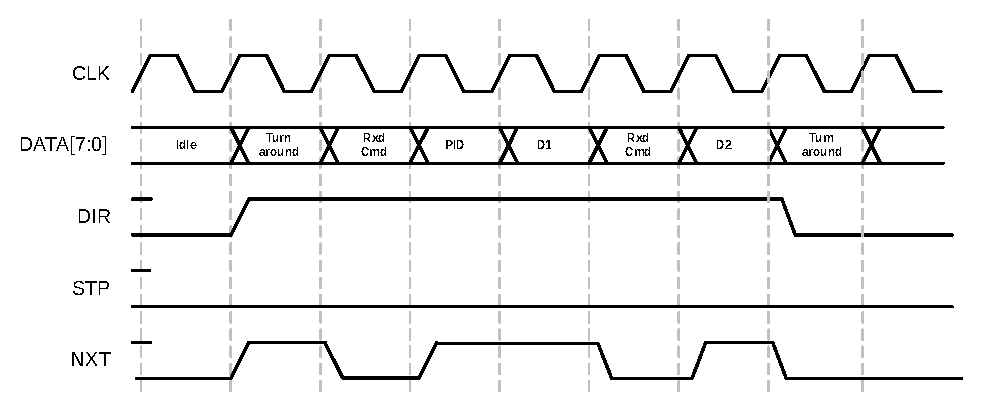
\includegraphics[width=90mm]{datasheets/USB3300_RECV.eps}
    \caption{Trama ULPI de recepción de datos USB.}
    \label{fig:ULPI_RECV}
\end{figure}



%* Comprobar
\section{Implementación de un sistema que gestione el envío de datos}
Diseño e implementación de un módulo en lenguaje Verilog, que gestione el envío al PC de los datos capturados. Además, sería interesante añadir una memoria intermedia en la que almacenar los datos antes de su envío, aminorando posibles perdidas.



%* Comprobar
\section{Implementación de un sistema que gestione los comandos entrantes}
Diseño e implementación de un módulo en lenguaje Verilog, que ante cualquier petición realizada por el usuario por el puerto serie anterior, deberá ser capaz de procesarla, obteniendo sus diversas partes (por ejemplo, dirección y datos en una petición de escritura de registro) y las almacenará temporalmente hasta que se puedan ejecutar.



% %* Comprobar
% \section{Implementación de un sistema que gestione todos los módulos}
% Una vez todos los módulos anteriores estén finalizados, es necesaria una sincronización entre todos ellos que permita obtener el resultado deseado. Por ello, se diseñará un módulo que envíe las señales de control pertinentes al resto de módulos dependiendo de las diversas entradas o registros internos de control.



%* Comprobar
\section{Creación de una aplicación de control}
Tras la finalización de la parte \emph{hardware}, es necesaria una aplicación, que conectándose por medio del puerto serie anteriormente implementado, sea capaz de en primer lugar enviar los diversos comandos necesarios para el correcto funcionamiento del sistema, y en segundo lugar, reciba los datos capturados de interés.

Debe ser como mínimo capaz de realizar las siguientes tareas.
\begin{itemize}
    \item Proveer de una sencilla interfaz en la que controlar todos los aspectos del sistema de captura.
    \item Controlar y procesar los datos entrantes y salientes del puerto serie.
    \item Almacenar los datos capturados en un archivo que permita un fácil análisis futuro, preferiblemente \emph{PCAP}\cite{tcpdump:pcap}.
\end{itemize}



% \section{Limitaciones en su ...}
% A la hora de desarrollar todos los objetivos anteriores, hay que tener presente todas aquellas limitaciones, principalmente los impuestos por la FPGA.

% \begin{itemize}
%     \item Existencia de unicamente 16 bloques de RAM de $4Kbits$ cada uno.
%     \item 
% \end{itemize}


% \chapter{Objetivos}
% \label{ch:objetivos-plantilla}

% Primero enumera los objetivos, no los resumas ni los redactes en un párrafo.  Cada uno de los objetivos de un proyecto debe ser SMART:

% \begin{description}
% \item[Simple] Cada objetivo tiene que ser independiente, tener sentido por sí mismo y más o menos indivisible.  Si no es suficientemente indivisible, pero tiene sentido como una entidad independiente, debes descomponerlo en subobjetivos.
% \item[Medible] Tiene que ser posible medir el grado de consecución al final del TFG.
% \item[Acordado] Los objetivos no los pones tú solo.  Deben partir de un acuerdo con tu director.
% \item[Realista] No pongas objetivos muy ambiciosos. Basta con que resuelva el problema de la forma más simple posible.  Si superas los objetivos nadie se va a quejar.  El director se encargará de que tampoco sean demasiado poco ambiciosos.
% \item[Temporizado] Un objetivo debe tener un marco temporal. Si no es así el objetivo podría no cumplirse nunca.  Es difícil poner límites temporales muy estrictos en un primer proyecto de ingeniería, pero al menos acota.
% \end{description}

% Tras cada objetivo puedes añadir párrafos ampliando la descripción del objetivo, describiendo los límites y justificándolos.  También puedes describir de qué se parte.  Si es posible debería quedar plenamente justificado que se trata de objetivos SMART.  Considera tanto límites intrínsecos (inherentes a la definición del proyecto) como extrínsecos (limitaciones presupuestarias, equipamiento disponible, etc). %* Listo [5/06 - 5/06]
\chapter{Contribuciones}
\label{ch:contribuciones}

%* Comprobar
Durante el proceso de diseño del sistema de la FPGA, y ante la necesidad de crear módulos o bloques funcionales de utilidad en lenguaje Verilog\cite{stuartsutherland2001}, se siguen una serie de procedimientos definidos desde un comienzo. Gracias a su uso, a parte de establecer unos mínimos requerimientos de calidad, se obtienen con mayor eficiencia los resultados buscados, permitiendo a su vez una alta legibilidad del código, y una buena capacidad de modificación y reutilización.

Para garantizarlo, estos procedimientos deben de ser comunes en todos los módulos, e invariables a lo largo del proyecto.



%* Comprobar
\section{Etapas de diseño de un módulo}
\label{ch:contribuciones:etapas}
%* Comprobar
En primer lugar, tras requerir la utilización de un módulo que logre una función específica, se analiza la posibilidad de reutilizar uno o varios módulos anteriormente realizados, evitando así un derroche innecesario de tiempo y recursos.

%* Comprobar
Seguidamente, se estudia la complejidad del módulo a desarrollar, dividiendolo, si fuera necesario, en varios submódulos con funciones más concretas que disminuyan el grado de dificultad general en su elaboración, permitiendo a su vez una mayor reutilización futura de código.

%* Comprobar
Estando definida ya su distribución, se realiza un pequeño esquema sobre el que partir, que de forma gráfica muestre sus diversas partes y relaciones, junto a este, si fuera necesario, se dibuja otro que muestre las etapas de la máquina de estados, pudiendo a continuación empezar con la programación del mismo.

Cada módulo dispone de un estilo común, distribuido de la siguiente forma:
\begin{enumerate}
    %* Comprobar
    \item{\textbf{Comentario de cabecera.}} \\
    Tal como se muestra en el listado~\ref{src:metodologia-verilog-cabecera}, se nombra al módulo, incluyendo una descripción breve de sus funciones. Además, se enumeran y explican todas las entradas, salidas, parámetros y estados de los que está formado.
    \begin{lstlisting}[language=Verilog,
        caption={Ejemplo de comentario de cabecera del módulo.},
        label=src:metodologia-verilog-cabecera]
/*
 * <Nombre del modulo> module
 * <Descripcion del modulo>
 *
 * Parameters:
 *  - <Nombre del parametro>. <Descripcion del parametro>
 *  - etc ..
 *
 * Inputs:
 *  - <Nombre de la entrada>. <Descripcion de la entrada>
 *  - etc ..
 *
 * Outputs:
 *  - <Nombre de la salida>. <Descripcion de la salida>
 *  - etc ..
 *
 * States:
 *  - <Nombre del estado>. <Descripcion del estado>
 *  - etc ..
 */
    \end{lstlisting}

    %* Comprobar
    \item{\textbf{Control de reinicio síncrono/asíncrono (listado~\ref{src:metodologia-verilog-sync}).}} \\
    Se trata de un pequeño bloque que controla la forma de funcionamiento de los reinicios. Si en el archivo principal se define la constante \emph{ASYNC\_RESET}, entonces todos los reinicios serán asíncronos, en caso contrario, serán síncronos a la señal de reloj (\emph{clk}).
    \begin{lstlisting}[language=Verilog,
        caption={Ejemplo de control de reinicio síncrono/asíncrono.},
        label=src:metodologia-verilog-sync]
// X es el nombre del modulo en cada caso
`ifdef ASYNC_RESET
    `define X_ASYNC_RESET or negedge rst
`else
    `define X_ASYNC_RESET
`endif
    \end{lstlisting}
        
    %* Comprobar
    \item{\textbf{Incorporación de módulos necearios (listado~\ref{src:metodologia-verilog-include-modules}).}} \\
    Suele ser habitual, que el módulo que se está desarrollando haga uso de otros, los cuales son incorporar en este momento.
    \begin{lstlisting}[language=Verilog,
        caption={Ejemplo de incorporación de módulos.},
        label=src:metodologia-verilog-include-modules]
`include "./modules/nombre_del_modulo.vh"
\\ etc ..
    \end{lstlisting}
        
    %* Comprobar
    \item{\textbf{Creación del módulo (listado~\ref{src:metodologia-verilog-create}).}} \\
    Se define el módulo, agrupando las entradas y salidas según características similares, posicionando en primer lugar las entradas, seguido de las salidas.
    \begin{lstlisting}[language=Verilog,
        caption={Ejemplo de creación de módulo.},
        label=src:metodologia-verilog-create]
module nombre_modulo
    #(
      parameter nombre_parametro = valor_parametro
      \\ etc ..
     )
     (
      // <Nombre del primer grupo de entradas/salidas>
      input  wire nombre_entrada_1, // <breve descripcion>
        // etc ..
      output wire nombre_salida_1,  // <breve descripcion>
        // etc ..
     );
    \end{lstlisting}
    
    %* Comprobar
    \item{\textbf{Inicialización de módulos necesarios (listado~\ref{src:metodologia-verilog-mod-init}).}} \\
    Todos los módulos incorporados previamente necesitan ser inicializados, relacionando sus entradas/salidas con el resto de señales del módulo.
    \begin{lstlisting}[language=Verilog,
        caption={Ejemplo inicialización de módulos.},
        label=src:metodologia-verilog-mod-init]
// Ejemplo inicializando el modulo clk\_baud\_pulse, que tiene dos parametros, una entrada y dos salidas
clk_baud_pulse #(
                 .COUNTER_VAL(BAUDS),
                 .PULSE_DELAY(BAUDS/2)
                )
   clk_baud_Rx  (
                 .clk_in(clk),       // Input
                 .clk_pulse(clk_Rx), // Output
                 .enable(enable)     // Output
                );
    \end{lstlisting}
    
    %* Comprobar
    \item{\textbf{Creación de los registros de control (listado~\ref{src:metodologia-verilog-regs}).}} \\
    Se crean todos los registros encargados de controlar el módulo o almacenar las variables.
    \begin{lstlisting}[language=Verilog,
        caption={Ejemplo de creación de registros.},
        label=src:metodologia-verilog-regs]
// Control registers
reg [1:0]X_state_r   = 2'b0; // Register that stores the current X state
reg [3:0]X_counter_r = 4'b0; // Register that counts ...
reg [7:0]DATA_buff   = 8'b0; // Buffer where ...
    \end{lstlisting}

    %* Comprobar
    \item{\textbf{Creación de \textit{flags} o señales de control (listado~\ref{src:metodologia-verilog-flags}).}} \\
    Para poder identificar con facilidad si el sistema se encuentra en un estado concreto, se crean estas señales, cuyo valor será \textit{1} cuando la máquina de estados esté en dicho estado, y \textit{0} en caso contrario.
    \begin{lstlisting}[language=Verilog,
        caption={Ejemplo de creación de \textit{flags}.},
        label=src:metodologia-verilog-flags]
// Flags
wire X_s_IDLE; // HIGH if X\_state\_r == X\_IDLE, else LOW
wire X_s_RUN;  // HIGH if X\_state\_r == X\_RUN,  else LOW
    \end{lstlisting}

    %* Comprobar
    \item{\textbf{Asignación de valores de salida y señales internas (listado~\ref{src:metodologia-verilog-asignacion}).}} \\
    Se asignan los valores que tomarán los diversos \emph{wires}, tanto de uso interno, como de salida, estos pueden relacionarse con registros, salidas de módulos ya inicializados u otros \emph{wires}. Además, al final de cada asignación, se comenta cual va a ser su uso, por ejemplo, una asignación de salida o control.
    \begin{lstlisting}[language=Verilog,
        caption={Ejemplo de asignación de valores.},
        label=src:metodologia-verilog-asignacion]
// Assigns
assign X_s_IDLE = (X_state_r == X_IDLE) ? 1'b1 : 1'b0; // \#FLAG
assign X_s_RUN  = (X_state_r == X_RUN)  ? 1'b1 : 1'b0; // \#FLAG

assign nombre_salida_1 = DATA_buff[2]; // \#OUTPUT
    \end{lstlisting}
    

    %* Comprobar 
    \item{\textbf{Enumeración de estados (listado~\ref{src:metodologia-verilog-estados}).}} \\
    Se crean tantos parámetros locales como estados tenga el módulo, cada uno con un valor identificativo único.
    \begin{lstlisting}[language=Verilog,
        caption={Ejemplo de enumeración de estados.},
        label=src:metodologia-verilog-estados]
/// X States (See module description at the beginning of this file to get more info)
localparam X_IDLE = 1'b0;
localparam X_RUN  = 1'b1;
    \end{lstlisting}
    

    %* Comprobar
    \item{\textbf{Máquina de estados (listado~\ref{src:metodologia-verilog-fst}).}} \\
    Se fijan y distribuyen los diversos caminos que puede tomar el sistema. Para ello se realiza una máquina de estados \emph{Mealy}\cite{mealy1955method}, es decir, los nuevos estados dependen de las entradas y del propio estado actual. Un pequeño ejemplo de una máquina de estados se muestra en el listado \ref{src:metodologia-verilog-fst}
    \begin{lstlisting}[language=Verilog,
        caption={Ejemplo de máquina de estados.},
        label=src:metodologia-verilog-fst]
always @(posedge clk `X_ASYNC_RESET) begin
    if(!rst) X_state_r <= X_IDLE;
    else begin
        case(X_state_r)
            X_IDLE: begin
                if(!nombre_entrada_1) X_state_r <= X_RUN;
                else                  X_state_r <= X_IDLE;
            end
            X_RUN: begin
                X_state_r <= X_IDLE;
            end
            default: X_state_r <= X_IDLE;
        endcase
    end
end
    \end{lstlisting}

    %* Comprobar
    \item{\textbf{Actualización de registros (listado~\ref{src:metodologia-verilog-act-regs}).}} \\
    Por último, se actualizan los valores de los registros del módulo, teniendo en cuenta que se trata de una máquina de estados \emph{Mealy}\cite{barkalov2005design}.
    \begin{lstlisting}[language=Verilog,
        caption={Ejemplo de actualización de registros.},
        label=src:metodologia-verilog-act-regs]
always @(posedge clk `UART_RX_ASYNC_RESET) begin
    if(!rst) begin
        X_counter_r <= 0;
    end
    else if(X_s_IDLE) begin
        X_counter_r <= X_counter_r - 1'b1;
    end
    else if(X_s_RUN) begin
        X_counter_r <= X_counter_r + 1'b1;
    end
end
    \end{lstlisting}
\end{enumerate}



%* Comprobar
\section{Pruebas y simulaciones}
\label{ch:contribuciones:pruebas}
%* Comprobar
Para asegurar el correcto funcionamiento de cada módulo, estos deben superar varias pruebas que comprueben cada una de sus funcionalidades. En caso de superar todas ellas satisfactoriamente, el módulo estaría listo para ser usado en la síntesis de la FPGA, en caso contrario, tendría que volver a la fase de desarrollo, en la que buscar y solventar los fallos, utilizando los resultados de las simulaciones realizadas.

%* Comprobar
Estás pruebas hacen uso de las herramientas de código abierto \emph{Icarus Verilog}\footnote{Véase su repositorio: \url{https://github.com/steveicarus/iverilog}} (abreviado \emph{iverilog}), encargada de simular el propio código de \emph{Verilog}, y el visor de ondas \emph{GTKWave}\cite{gtkwave2019}, permitiendo generar y mostrar gráficamente todas las señales del circuito en cualquier instante de tiempo.

%* Comprobar
Para llevar a cabo dicha simulación, \emph{Iverilog} tiene como entrada un archivo en lenguaje \emph{Verilog} en el que se inicializa el propio módulo a analizar, y seguidamente, en ese mismo archivo, se van variando las entradas al módulo según su instante de tiempo. Posteriormente, y tras obtener el archivo con el resultado de la simulación, se abre en \emph{GTKWave} y se compara el resultado generado en el módulo, respecto al esperado.

En la figura~\ref{fig:ej-gtkwave} se muestra el resultado gráfico de una simulación de ejemplo.

\begin{figure}[htb]
    \centering
    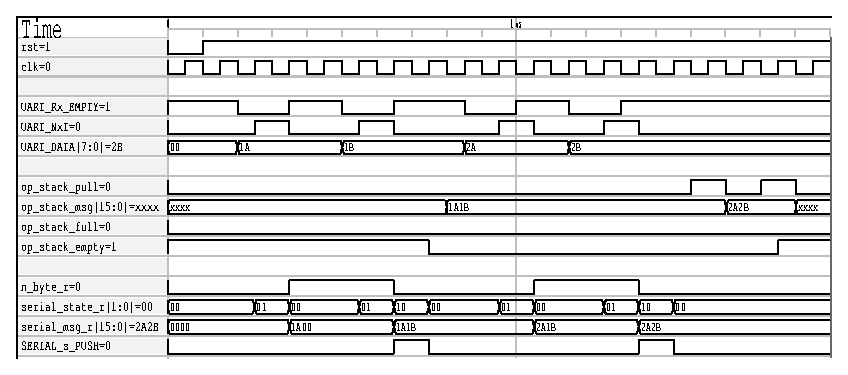
\includegraphics[width=120mm]{otro/ej_simulacion_gtkwave.eps}
    \caption{Ejemplo del resultado de una simulación en \emph{GTKWave}.}
    \label{fig:ej-gtkwave}
\end{figure}


%* Comprobar
\section{Distribución de archivos}
\label{ch:contribuciones:archivos}
Todo el código fuente utilizado por el sistema de la FPGA sigue una estructura concreta, reflejada en la figura~\ref{fig:tree-fpga}.
\begin{figure}[hbtp]
    \centering
    \begin{minipage}{11cm}
        \dirtree{%
            .1 ./.
            .2 modules/     \ldots{}
                            \begin{minipage}[t]{7cm}
                                \begin{flushright}
                                    Carpeta que contiene todos los módulos diseñados
                                \end{flushright}
                            \end{minipage}.
            .3 modulo\_1/.
            .4 rtl/.
            .4 tb/.
            .3 modulo\_2/.
            .4 rtl/.
            .4 tb/.
            .3 modulo\_1.vh     \ldots{}
                                \begin{minipage}[t]{6cm}
                                    \begin{flushright}
                                        Cada módulo diseñado debe tener un archivo de cabecera utilizado para inicializarlo
                                    \end{flushright}
                                \end{minipage}.
            .3 modulo\_2.vh.
            .3 ....
            .2 modules\_simulation/     \ldots{}
                                        \begin{minipage}[t]{5.2cm}
                                            \begin{flushright}
                                                Módulos usados unicamente en la simulación
                                            \end{flushright}
                                        \end{minipage}.
            .3 SB\_PLL40\_CORE.
            .3 SB\_RAM40\_4K/.
            .3 SB\_PLL40\_CORE.vh.
            .3 SB\_RAM40\_4K.vh.
            .2 rtl/     \ldots{}
                        \begin{minipage}[t]{7cm}
                            \begin{flushright}
                                Archivos principales del sistema
                            \end{flushright}
                        \end{minipage}.
            .3 bauds.vh/.
            .3 top.pcf/     \ldots{}
                            \begin{minipage}[t]{6.6cm}
                                \begin{flushright}
                                    Archivo que une los pines físicos con la lógica interna
                                \end{flushright}
                            \end{minipage}.
            .3 top.v/       \ldots{}
                            \begin{minipage}[t]{7cm}
                                \begin{flushright}
                                    Archivo Verilog principal
                                \end{flushright}
                            \end{minipage}.
            .2 tb/.
            .3 top\_tb.v/       \ldots{}
                                \begin{minipage}[t]{6.5cm}
                                    \begin{flushright}
                                        Archivo que simula el sistema en su conjunto
                                    \end{flushright}
                                \end{minipage}.
            .2 Makefile     \ldots{}
                            \begin{minipage}[t]{7cm}
                                \begin{flushright}
                                    Archivo de automatización de tareas
                                \end{flushright}
                            \end{minipage}.
        }
    \end{minipage}
    \caption{Estructura de carpetas del código de la FPGA}
    \label{fig:tree-fpga}
\end{figure}


% \chapter{Contribuciones}
% \label{ch:contribuciones-plantilla}

% Tus contribuciones no tienen por qué limitarse al trabajo sistemático del TFG.  Puede que hayas contribuido en aspectos metodológicos, en ideas novedosas, en la planificación de experimentos, en desarrollos matemáticos.

% Este capítulo está para agrupar todo eso.  Describe con claridad, y sin suponer conocimiento previo del desarrollo del proyecto (que viene después) todo lo que ha supuesto contribuciones originales por tu parte. %* Listo [6/06 - 7/06]
\chapter{Procedimiento}
\label{ch:procedimiento}

%! 
\noWord[Modificar lo que sea necesario, añadir captura Trello??, recalcar alguna cosa]

%* Comprobar
En el desarrollo del presente TFG se ha utilizado una metodología ágil basada en \emph{Scrum}~\cite{scrumguide}, definida por el director. El trabajo se ha dividido en iteraciones de varias semanas denominadas \emph{sprints}. Las unidades de trabajo se presentan en forma de historias de usuario (\emph{user stories}) que definen mini-proyectos de muy corta duración que aportan valor al proyecto.  Es decir, cada historia de usuario cumple o ayuda a cumplir alguno de los objetivos. Medir el valor percibido corresponde al propietario del producto (\emph{Product Owner}), que participa activamente en la planificación del proceso priorizando las unidades de trabajo.


%!
\section{Diferencias con Scrum}
%!
\emph{Scrum} es una metodología estrictamente centrada en el cliente. El cliente es el responsable de priorizar y, en cierto modo, planificar las iteraciones. Esto garantiza que la ejecución del proyecto responda al máximo con las expectativas del cliente, aún cuando los imprevistos impidan alcanzar alguno de los objetivos iniciales. Esta característica de \emph{Scrum} es la única que se ha intentado mantener inalterada. Sin embargo, al ser el TFG un proyecto individual, ha requerido modificar significativamente otros aspectos de la metodología.

%!
\subsection{Roles}
La única remuneración que se obtiene con la ejecución de un TFG es la calificación de los distintos aspectos (anteproyecto, valoración del director, valoración del tribunal, etc.).  Por tanto, el cliente del TFG se compone por el director y el tribunal de la defensa.  Desgraciadamente no es posible conocer a priori el tribunal.  Por este motivo el director es el único representante del cliente en el proceso de desarrollo (\emph{Product Owner}).

Al ser el TFg realizado de manera individual, el equipo de trabajo (\emph{Team Member}) se compone exclusivamente por el autor.

La labor de dirección del TFG se asimila a la de dirección del proyecto y, por tanto, el director también actúa como coordinador del proceso, o \emph{Scrum Master}.  Nótese que hay dos roles representados por la misma persona.  Desde un punto de vista purista esto implica que puede haber conflicto de intereses y los intereses del cliente pueden estar insuficientemente representados.  Es una limitación extrínseca, que no es posible solucionar con el proceso actual.  Aún así, el uso de una metodología ágil centrada en el cliente debe mejorar el alineamiento de intereses cuando sobrevienen problemas que afectan o pueden afectar a la consecución de alguno de los objetivos iniciales.

%!
\subsection{Historias de usuario}
\emph{Scrum}, como la mayoría de los métodos ágiles, está enfocada al desarrollo de proyectos en entornos de alta incertidumbre por equipos multidisciplinares bien formados.  El desarrollo de un TFG, al tratarse de un primer proyecto profesional, también está sometido a gran cantidad de incertidumbre.  Sin embargo, no siempre se cuenta con la formación previa necesaria para abordar todos los problemas.  Esto implica que, en ocasiones, se necesita aprender o leer, sin repercusión medible en el valor percibido por el \emph{Product Owner}.  En esos casos se planifican unidades de trabajo que no corresponden estrictamente a historias de usuario en el sentido de Scrum.  Se ha intentado mantener al mínimo este tipo de historias de usuario para tener el proceso lo más controlado posible.

Puntualmente ha sido necesario planificar historias de usuario que solo pretenden explorar opciones.  Este tipo de historias de usuario están contempladas en \emph{Scrum}, se denominan \emph{spikes}.  Sin embargo, en la ejecución de este TFG se ha procurado reducir al mínimo para que la exploración de alternativas no domine en el tiempo dedicado al TFG.

%!
\subsection{Planificación de sprints}
Para la planificación y el seguimiento se ha utilizado un tablero \href{http://trello.com}{Trello}.  Los tableros Trello permiten agrupar tarjetas en una serie de listas con nombre.  Se ha utilizado el esquema propuesto en~\cite{andrewlittlefield2016}.

El autor ha sido responsable de añadir la mayoría de las historias de usuario a la lista \emph{Backlog}.  Se trata de un proceso continuo, durante toda la ejecución del proyecto.  El director, como \emph{product owner}, prioriza las historias, moviendo las tarjetas dentro de la lista \emph{Backlog}.  Justo antes de cada iteración se realiza una reunión presencial o virtual para revisar la iteración pasada y planificar la siguiente iteración.

Usando la técnica de \emph{planning poker} (ver~\cite{scrumguide}) se dimensionan las historias de usuario en días de trabajo.  Esta técnica consiste en un proceso de generación de consenso entre el autor y el director sobre el tiempo requerido para la ejecución de cada historia de usuario.  La unidad empleada ha sido de un día.

El director, como \emph{product owner} traslada las tarjetas correspondientes a las primeras historias de la lista \emph{Backlog} a la lista \emph{ToDo} hasta completar los 10 días de trabajo de la iteración.

%!
\subsection{Flujo de trabajo}
El flujo de trabajo diario del autor corresponde a la siguiente secuencia:

\begin{itemize}
    \item Dentro de la lista \emph{ToDo} puede elegirse cualquier tarjeta para trabajar en ella.  Antes de comenzar el trabajo se arrastra la tarjeta a la lista \emph{Doing}.  Esto proporciona información en tiempo real al director del progreso de la iteración.
    
    \item Al terminar una historia de usuario la tarjeta correspondiente se arrastra a la lista \emph{QC} (quality control).
    
    \item El director, como \emph{Scrum Master}, revisa que la historia está realmente acabada y, si así es, la traslada a la lista \emph{Done}. En caso contrario la traslada a la lista \emph{Doing} otra vez, añadiendo un comentario que lo justifica.

    \item Si en el transcurso del trabajo se encuentra un obstáculo que impide progresar con una historia, se traslada a la lista \emph{Blocked}, añadiendo un comentario que lo justifica.
\end{itemize}

En todo momento es posible ver el estado global de ejecución del proyecto.  Al finalizar, la lista \emph{Done} contiene todas las historias de usuario ejecutadas por orden de terminación.  Y las listas \emph{Blocked} y \emph{Backlog} contienen (en este orden) todas las historias de usuario que corresponderían a trabajo futuro, ya priorizadas por el director.

%!
\subsection{Herramientas de ayuda}
El proceso de desarrollo está fuertemente ligado a la herramienta \href{https://trello.com/}{Trello}.  Se trata de una herramienta colaborativa en línea, que permite mantener una serie de tarjetas agrupadas en listas con nombre.  Cada tarjeta puede tener un título, una descripción, un conjunto de adjuntos, y un conjunto de comentarios.  Trello se ha usado con éxito en la planificación de proyectos de nivel de complejidad muy variable.  Por ejemplo, Epic Games utiliza un tablero Trello para planificar las características a incorporar a cada nueva versión de Unreal Engine.  Por otro lado, un problema de Trello es el manejo limitado de la historia de modificaciones en las tarjetas y en los movimientos entre listas de tarjetas.  Esto dificulta en cierto modo el seguimiento de los cambios y, sobre todo, la corrección de errores en el proceso.  Por este motivo, Trello solo se ha empleado en la coordinación del trabajo, mientras que toda la gestión de cambios se ha delegado en otra herramienta.

Todo el proyecto ha sido gestionado desde su inicio con una herramienta de control de versiones distribuido~\cite{scottchaconbenstraub2018} en un repositorio público de GitHub, disponible en \thegitrepo.  Cada vez que se completa con éxito una historia de usuario se notifica mediante un comentario en la tarjeta correspondiente.  Este comentario tan solo contiene el identificador del paquete de cambios (\emph{commit}) que da por concluida la historia.  Todos los \emph{stakeholders} pueden consultar la evolución del proyecto en todo momento desde la propia página del repositorio.

\warning{Es posible detallar en este capítulo las iteraciones desarrolladas.  Otra posibilidad es comentar brevemente los problemas encontrados y en el siguiente capítulo explicar los resultados globales.}

% \chapter{Procedimiento}
% \label{ch:procedimiento-plantilla}

% \info{Esta descripción está hecha a título orientativo. Puedes mejorarla con capturas de tu propio tableto Trello o con cualquier aclaración que consideres necesaria.}

% En el desarrollo de este TFG se ha utilizado una metodología ágil basada en \emph{Scrum}~\cite{scrumguide}, definida por el director.  El trabajo se ha dividido en iteraciones de dos semanas denominadas \emph{sprints}.  Las unidades de trabajo se presentan en forma de historias de usuario (\emph{user stories}) que definen mini-proyectos de muy corta duración que aportan valor al proyecto.  Es decir, cada historia de usuario cumple o ayuda a cumplir alguno de los objetivos.  Medir el valor percibido corresponde al propietario del producto (\emph{Product Owner}), que participa activamente en la planificación del proceso priorizando las unidades de trabajo.

% La utilización de una metodología ágil permite equilibrar la cantidad de trabajo y los objetivos alcanzados.  Los 12 créditos ECTS del TFG se reparten según el criterio del director para que los resultados aporten el máximo valor posible, incluso en presencia de imprevistos.

% \section{Diferencias con Scrum}

% \emph{Scrum} es una metodología estrictamente centrada en el cliente.  El cliente es el responsable de priorizar y, en cierto modo, planificar las iteraciones.  Esto garantiza que la ejecución del proyecto responde al máximo con las expectativas del cliente, aún cuando los imprevistos impidan alcanzar alguno de los objetivos iniciales.  Esta característica de \emph{Scrum} es la única que se ha intentado mantener inalterada.  Sin embargo, el TFG es un proyecto individual, lo que ha requerido modificar significativamente otros aspectos de la metodología.

% \subsection{Roles}

% La única remuneración que se obtiene con la ejecución de un TFG es la calificación de los distintos aspectos (anteproyecto, valoración del director, valoración del tribunal, etc.).  Por tanto, el cliente del TFG se compone por el director y el tribunal de la defensa.  Desgraciadamente no es posible conocer a priori el tribunal.  Por este motivo el director es el único representante del cliente en el proceso de desarrollo (\emph{Product Owner}).

% El TFG debe ser realizado de manera individual.  Por tanto, el equipo de trabajo (\emph{Team Member}) se compone exclusivamente por el autor.

% La labor de dirección del TFG se asimila a la de dirección del proyecto y, por tanto, el director también actúa como coordinador del proceso, o \emph{Scrum Master}.  Nótese que hay dos roles representados por la misma persona.  Desde un punto de vista purista esto implica que puede haber conflicto de intereses y los intereses del cliente pueden estar insuficientemente representados.  Es una limitación extrínseca, que no es posible solucionar con el proceso actual.  Aún así, el uso de una metodología ágil centrada en el cliente debe mejorar el alineamiento de intereses cuando sobrevienen problemas que afectan o pueden afectar a la consecución de alguno de los objetivos iniciales.

% \subsection{Historias de usuario}

% \emph{Scrum}, como la mayoría de los métodos ágiles, está enfocada al desarrollo de proyectos en entornos de alta incertidumbre por equipos multidisciplinares bien formados.  El desarrollo de un TFG, al tratarse de un primer proyecto profesional, también está sometido a gran cantidad de incertidumbre.  Sin embargo, no siempre se cuenta con la formación previa necesaria para abordar todos los problemas.  Esto implica que, en ocasiones, se necesita aprender o leer, sin repercusión medible en el valor percibido por el \emph{Product Owner}.  En esos casos se planifican unidades de trabajo que no corresponden estrictamente a historias de usuario en el sentido de Scrum.  Se ha intentado mantener al mínimo este tipo de historias de usuario para tener el proceso lo más controlado posible.

% Puntualmente ha sido necesario planificar historias de usuario que solo pretenden explorar opciones.  Este tipo de historias de usuario están contempladas en \emph{Scrum}, se denominan \emph{spikes}.  Sin embargo, en la ejecución de este TFG se ha procurado reducir al mínimo para que la exploración de alternativas no domine en el tiempo dedicado al TFG.

% \subsection{Planificación de sprints}

% Para la planificación y el seguimiento se ha utilizado un tablero \href{http://trello.com}{Trello}.  Los tableros Trello permiten agrupar tarjetas en una serie de listas con nombre.  Se ha utilizado el esquema propuesto en~\cite{andrewlittlefield2016}.

% El autor ha sido responsable de añadir la mayoría de las historias de usuario a la lista \emph{Backlog}.  Se trata de un proceso continuo, durante toda la ejecución del proyecto.  El director, como \emph{product owner}, prioriza las historias, moviendo las tarjetas dentro de la lista \emph{Backlog}.  Justo antes de cada iteración se realiza una reunión presencial o virtual para revisar la iteración pasada y planificar la siguiente iteración.

% Usando la técnica de \emph{planning poker} (ver~\cite{scrumguide}) se dimensionan las historias de usuario en días de trabajo.  Esta técnica consiste en un proceso de generación de consenso entre el autor y el director sobre el tiempo requerido para la ejecución de cada historia de usuario.  La unidad empleada ha sido de un día.

% El director, como \emph{product owner} traslada las tarjetas correspondientes a las primeras historias de la lista \emph{Backlog} a la lista \emph{ToDo} hasta completar los 10 días de trabajo de la iteración.

% \subsection{Flujo de trabajo}

% El flujo de trabajo diario del autor corresponde a la siguiente secuencia:

% \begin{itemize}
%     \item Dentro de la lista \emph{ToDo} puede elegirse cualquier tarjeta para trabajar en ella.  Antes de comenzar el trabajo se arrastra la tarjeta a la lista \emph{Doing}.  Esto proporciona información en tiempo real al director del progreso de la iteración.
    
%     \item Al terminar una historia de usuario la tarjeta correspondiente se arrastra a la lista \emph{QC} (quality control).
    
%     \item El director, como \emph{Scrum Master}, revisa que la historia está realmente acabada y, si así es, la traslada a la lista \emph{Done}. En caso contrario la traslada a la lista \emph{Doing} otra vez, añadiendo un comentario que lo justifica.

%     \item Si en el transcurso del trabajo se encuentra un obstáculo que impide progresar con una historia, se traslada a la lista \emph{Blocked}, añadiendo un comentario que lo justifica.
% \end{itemize}

% En todo momento es posible ver el estado global de ejecución del proyecto.  Al finalizar, la lista \emph{Done} contiene todas las historias de usuario ejecutadas por orden de terminación.  Y las listas \emph{Blocked} y \emph{Backlog} contienen (en este orden) todas las historias de usuario que corresponderían a trabajo futuro, ya priorizadas por el director.

% \subsection{Herramientas de ayuda}

% El proceso de desarrollo está fuertemente ligado a la herramienta \href{https://trello.com/}{Trello}.  Se trata de una herramienta colaborativa en línea, que permite mantener una serie de tarjetas agrupadas en listas con nombre.  Cada tarjeta puede tener un título, una descripción, un conjunto de adjuntos, y un conjunto de comentarios.  Trello se ha usado con éxito en la planificación de proyectos de nivel de complejidad muy variable.  Por ejemplo, Epic Games utiliza un tablero Trello para planificar las características a incorporar a cada nueva versión de Unreal Engine.  Por otro lado, un problema de Trello es el manejo limitado de la historia de modificaciones en las tarjetas y en los movimientos entre listas de tarjetas.  Esto dificulta en cierto modo el seguimiento de los cambios y, sobre todo, la corrección de errores en el proceso.  Por este motivo, Trello solo se ha empleado en la coordinación del trabajo, mientras que toda la gestión de cambios se ha delegado en otra herramienta.

% Todo el proyecto ha sido gestionado desde su inicio con una herramienta de control de versiones distribuido~\cite{scottchaconbenstraub2018} en un repositorio público de GitHub, disponible en \thegitrepo.  Cada vez que se completa con éxito una historia de usuario se notifica mediante un comentario en la tarjeta correspondiente.  Este comentario tan solo contiene el identificador del paquete de cambios (\emph{commit}) que da por concluida la historia.  Todos los \emph{stakeholders} pueden consultar la evolución del proyecto en todo momento desde la propia página del repositorio.

% \warning{Es posible detallar en este capítulo las iteraciones desarrolladas.  Otra posibilidad es comentar brevemente los problemas encontrados y en el siguiente capítulo explicar los resultados globales.}
 %! Revisar
\chapter{Resultados}
\label{ch:resultados}

%* Comprobar
En el siguiente capitulo se van a comentar los diversos resultados obtenidos en el presente TFG, tanto los relacionados con la FPGA (\emph{hardware} usado, simulaciones y sintetizado final), como con el \emph{software} de control. Se incluyen además, varias imágenes que complementen las explicaciones del mismo.


%!
\section{Resultados de los elementos \emph{hardware} del sistema.}
%* Comprobar
Partiendo del esquema dado de analizadores USB \emph{hardware} (figura~\ref{fig:esquema-hardware}), se aprecian dos partes implicadas en la captura, por un lado el encargado de capturar la trama, y por otro, el encargado de controlar dicha captura y almacenar los resultados. En esta sección se van a comentar los resultados de la primera.

\begin{figure}[htb]
    \centering
    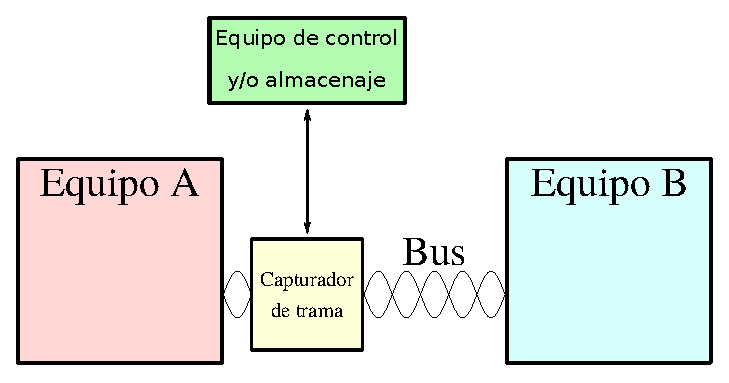
\includegraphics[width=70mm]{esquemas/esquema-captura-hardware-2.eps}
    \caption{Esquema de analizadores \emph{hardware}}
    \label{fig:esquema-hardware}
\end{figure}

%* Comprobar
\subsection{Componentes utilizados.}
En al figura \ref{fig:sistema_final} se muestra el resultado \emph{hardware} del presente trabajo, este a su vez, está formado por los siguientes componentes.

\begin{figure}[htbp]
    \centering
    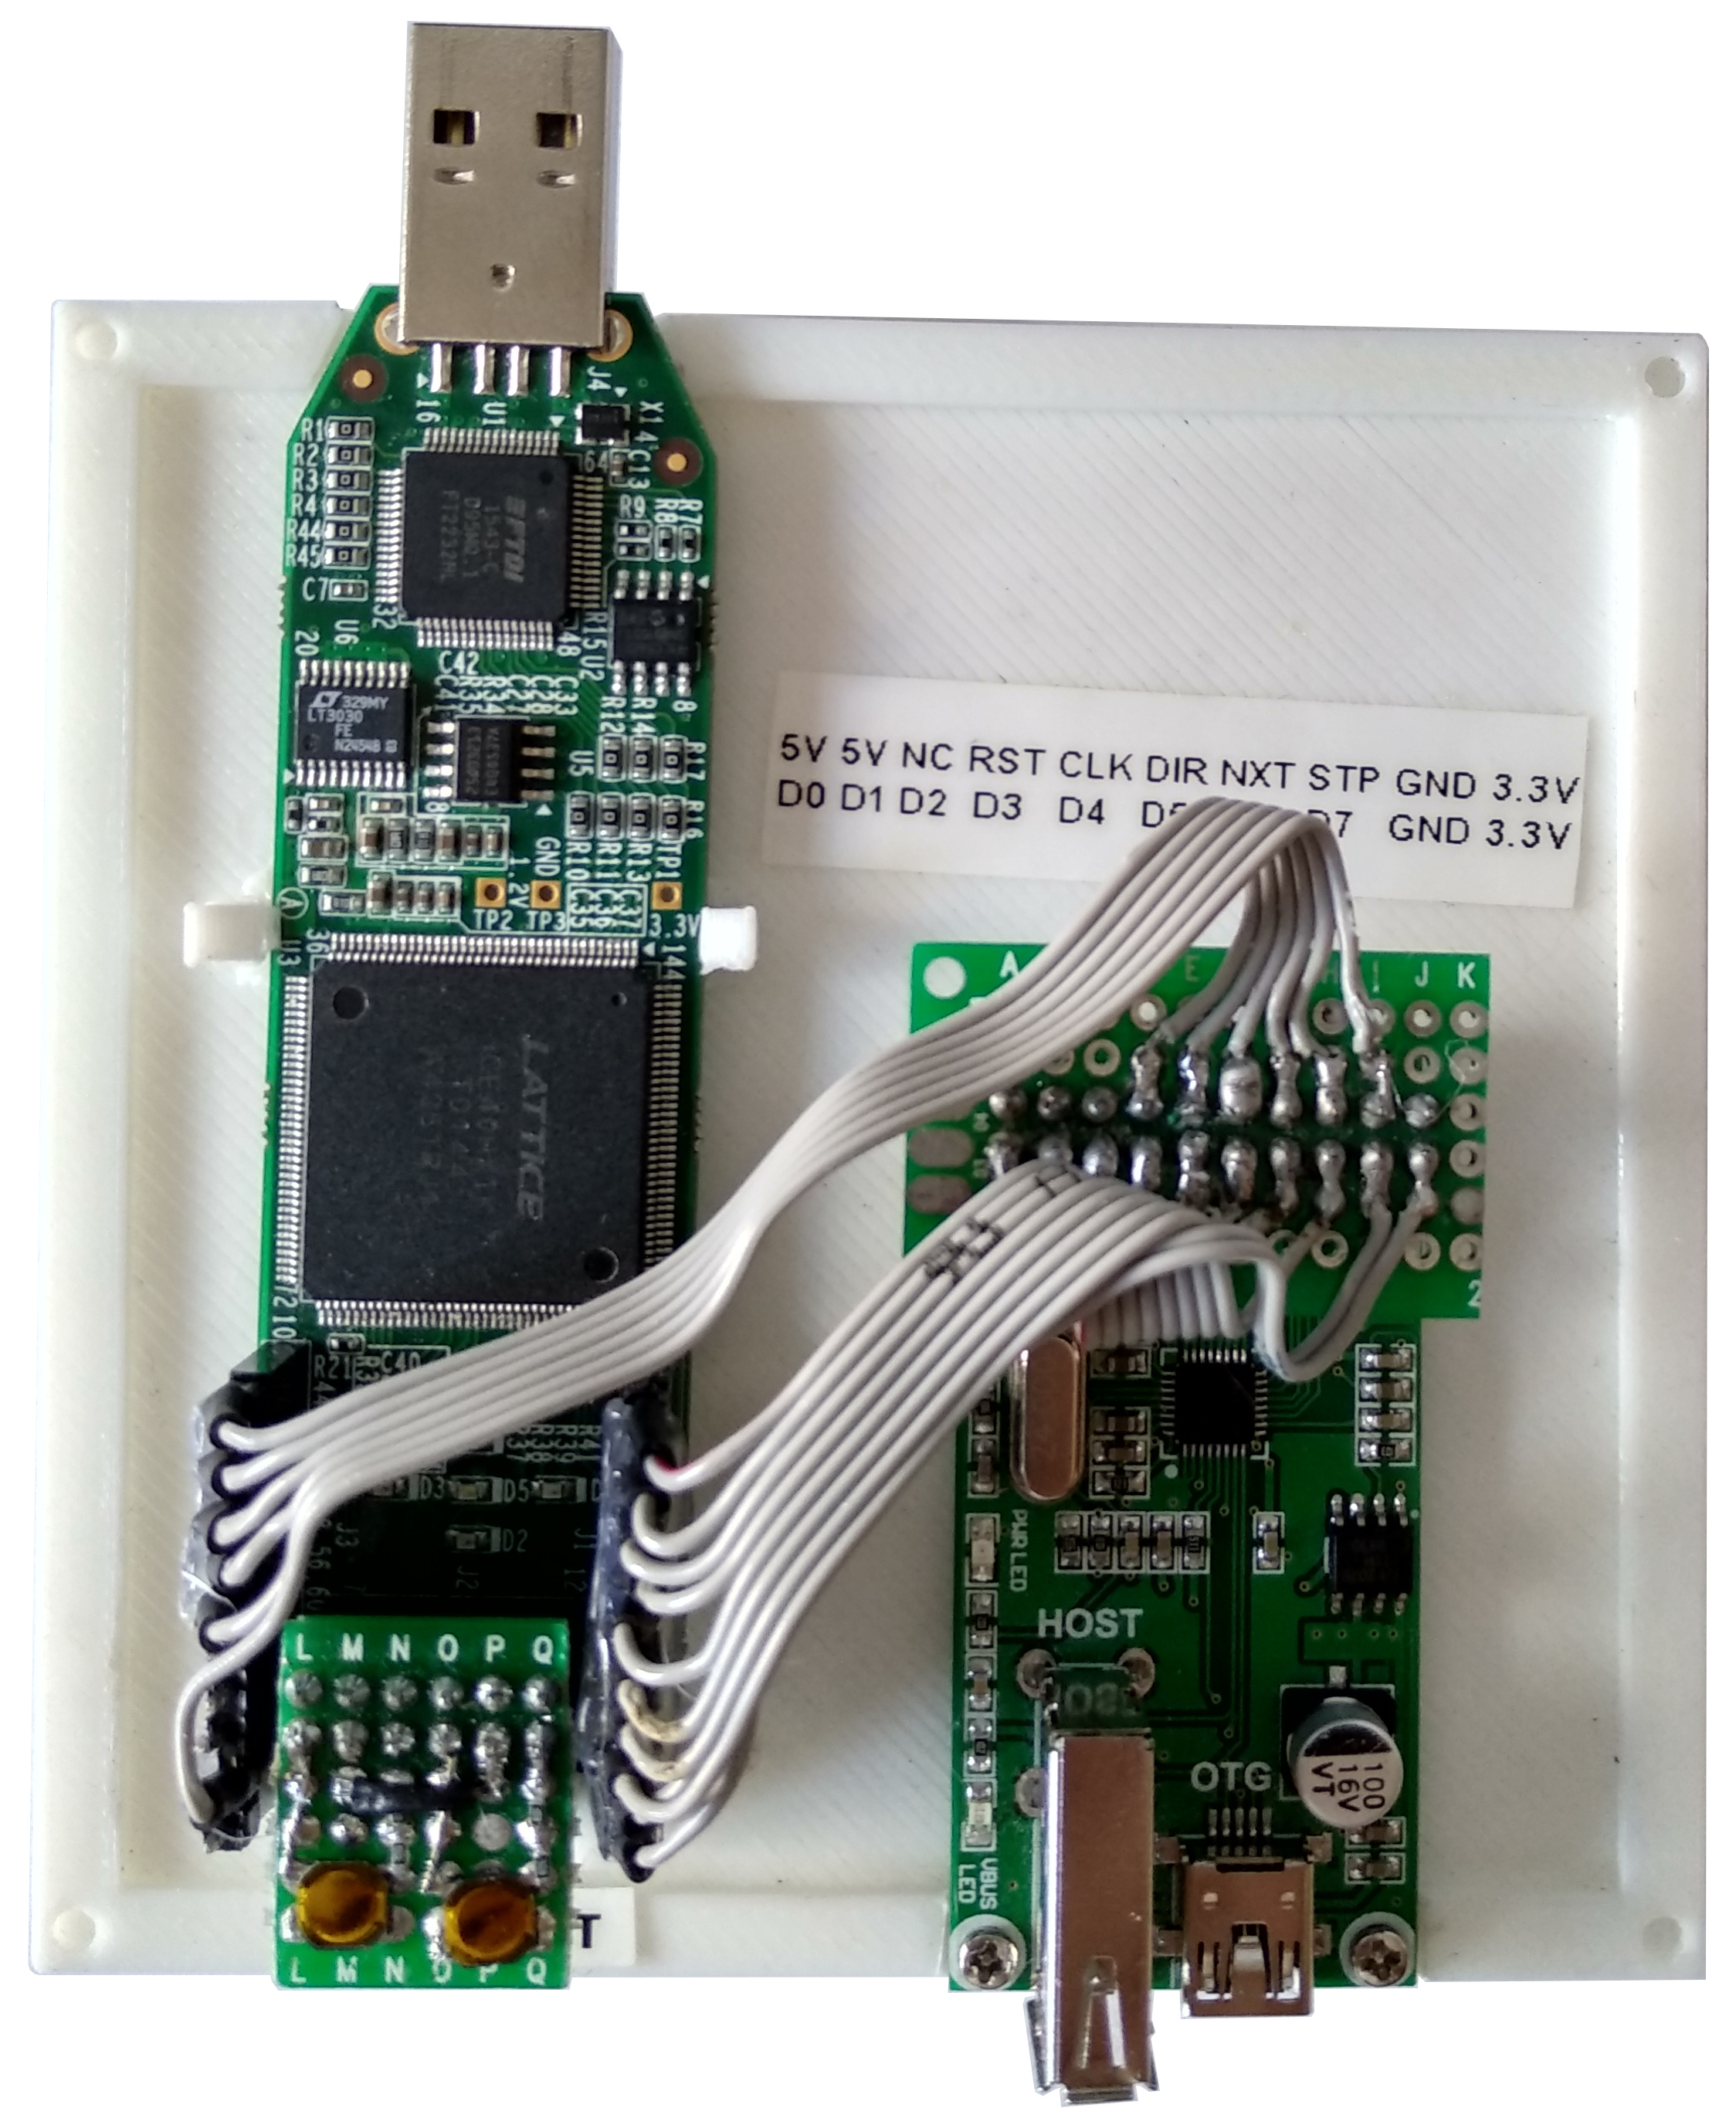
\includegraphics[height=110mm]{hw_final/final_cut.jpg}
    \caption{Sistema de captura final}
    \label{fig:sistema_final}
\end{figure}

\begin{enumerate}
    %* Comprobar
    \item \textbf{Placa de desarrollo \emph{IceStick \cite{icestickmanual}} (Véase figura~\ref{fig:IceStick_board}).} \\
    Se trata de una placa de desarrollo, que incorpora, sin contar con todos los conectores, indicadores \emph{LEDs}, elementos pasivos y componentes de regulación, la \emph{FPGA iCE40HX-1k \cite{lattice:ice40}} del fabricante \emph{Lattice}\footnote{Página web del producto: \url{https://www.latticesemi.com/Products/FPGAandCPLD/iCE40.aspx}}, memoria SPI de $32MBit$ para almacenar el sintetizado generado, conversor USB a doble puerto de comunicación FIFO \emph{FTDI 2232H \cite{FTDI:FT2232HL}} para comunicarse con el PC y oscilador de $12MHz$ con el que referenciar ciertas partes del circuito.
    
    \begin{figure}[htbp]
        \centering
        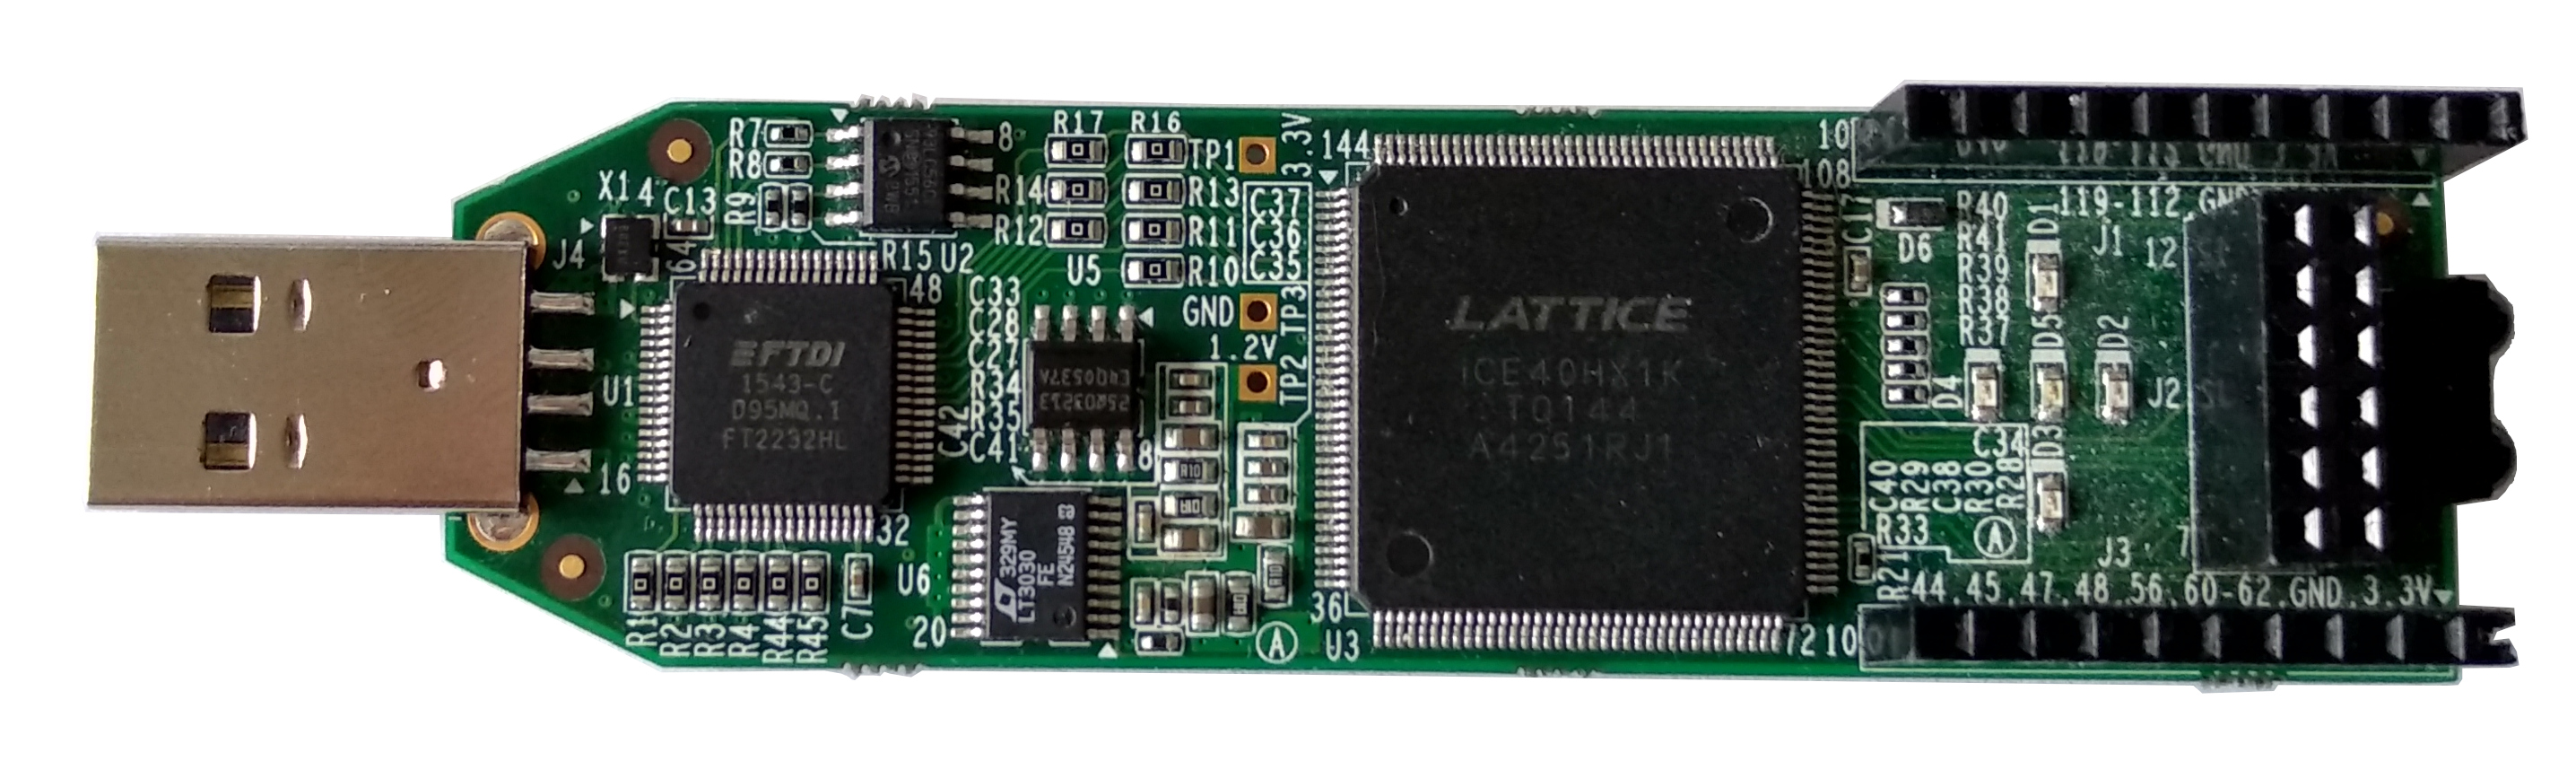
\includegraphics[width=125mm]{hw_final/IceStick_board_cut.jpg}
        \caption{Placa de desarrollo \emph{IceStick}}
        \label{fig:IceStick_board}
    \end{figure}

    %* Comprobar
    \item \textbf{Módulo encargado de la capa física USB.} \\
    PCB que incorpora el circuito integrado \emph{USB3300\cite{icestickmanual}} del fabricante \emph{Microchip}. Este se encarga de manejar la capa física del bus USB, comunicándose con la FPGA por medio del protocolo ULPI\cite{ulpi-specs}.

    En al figura~\ref{fig:USB3300_board}, se aprecia que dicha PCB incluye dos conectores USB, uno tipo A hembra, y otro tipo mini-B hembra. Sus señales de datos están interconectadas, por lo que es en este punto donde ambos extremos del bus a analizar se unen, pudiendo capturar la trama sin interrumpir la conexión debido a que, el integrado \emph{USB3300} se puede configurar para mantener sus patillas de datos en alta impedancia.

    \begin{figure}[htbp]
        \centering
        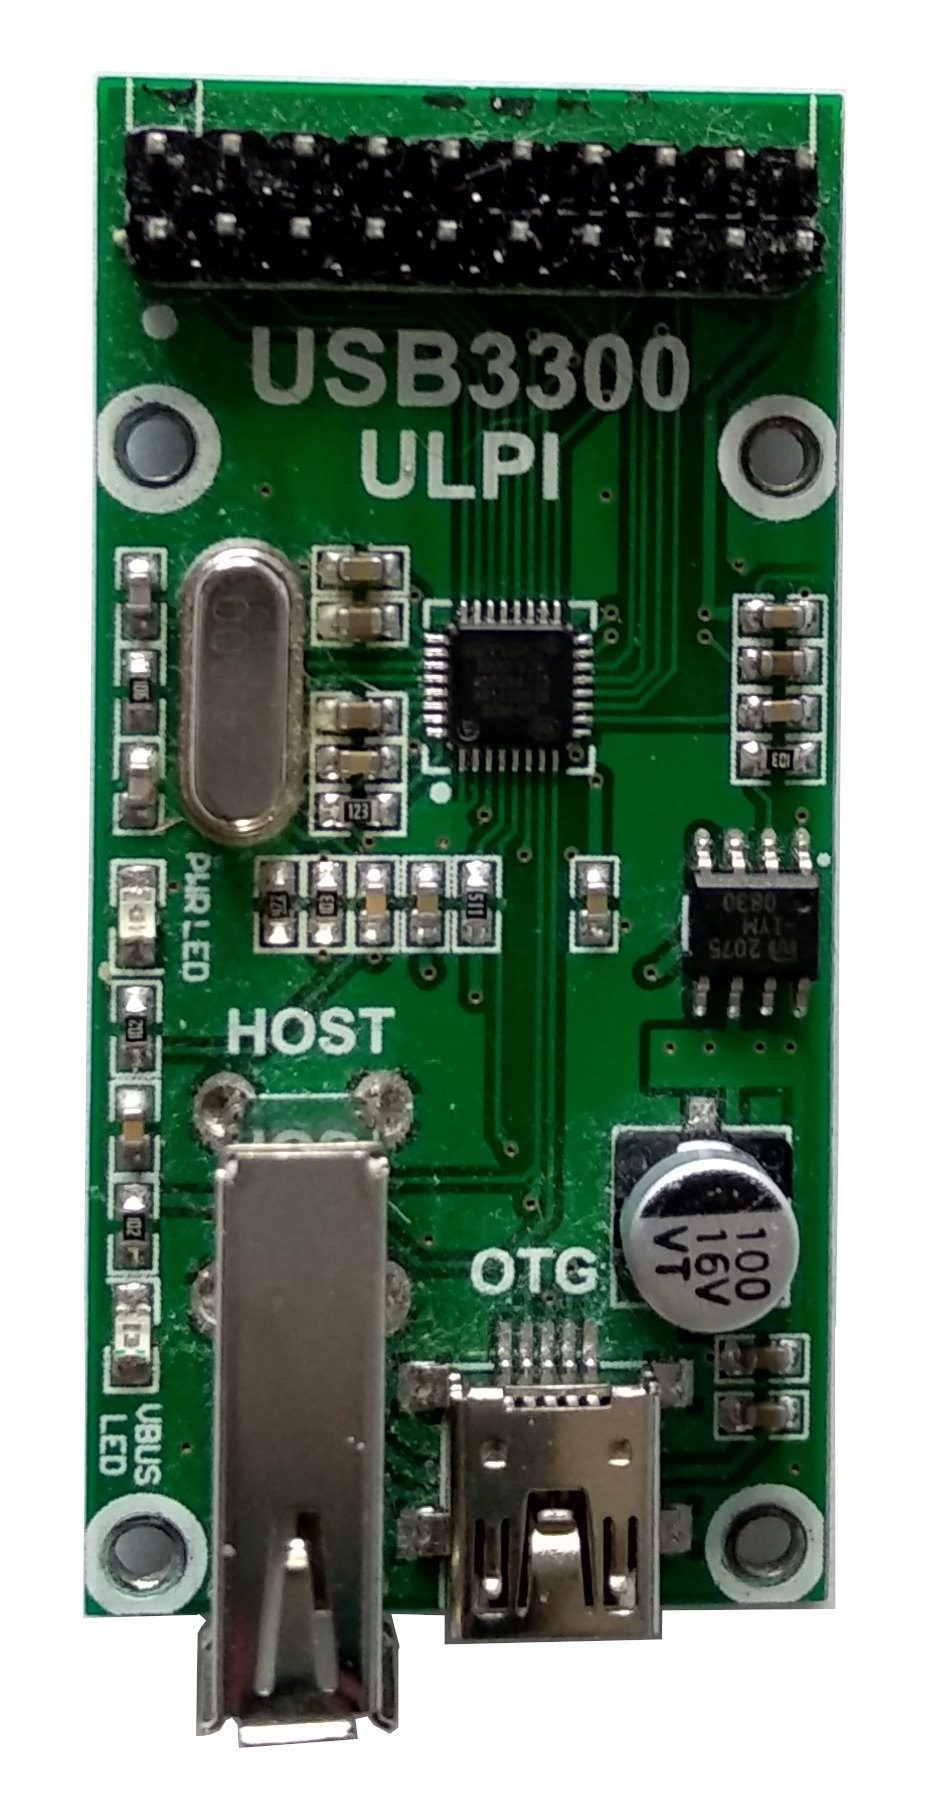
\includegraphics[width=50mm]{hw_final/USB3300_board_cut.jpg}
        \caption{PCB con el integrado \emph{USB3300}}
        \label{fig:USB3300_board}
    \end{figure}

    %* Comprobar
    \item \textbf{Cableado de unión (Figura~\ref{fig:matriz-hw-resto:cables}).} \\
    Para conexionar ambas placas, se utilizan varios cables entre el conector del módulo con el integrado \emph{USB3300} y los conectores laterales de la placa \emph{IceStick}.

    La \emph{FPGA iCE40HX-1k} posee 4 bancos de señales de entrada/salida, para evitar posibles retrasos en las señales\cite{fpga:routing}, los 8bits de datos paralelos se conectan al banco 0 (pines del 112 al 119), mientras que el resto de señales ULPI (DIR, STP, RST y NXT) al banco 2.
    
    %* Comprobar
    \item \textbf{Pulsadores externos (Figura~\ref{fig:matriz-hw-resto:botones}).} \\
    Se han incluido dos botones auxiliares externos, con los que poder tanto reiniciar el sistema en su totalidad, como enviar un $byte$ de prueba por el puerto serie.
    
    Las señales son activas a nivel bajo, por lo que se mantienen siempre a nivel alto por medio de unas resistencias de \emph{Pull-Up} (Figura~\ref{fig:buttons_circuit}).
    \begin{figure}[h]
        \centering
        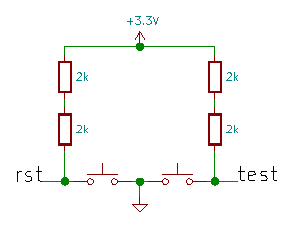
\includegraphics[width=50mm]{hw_final/buttons_circuit2.eps}
        \caption{Esquema de los botones auxiliares}
        \label{fig:buttons_circuit}
    \end{figure}

    %* Comprobar
    \item \textbf{Base impresa en 3D (Figura~\ref{fig:matriz-hw-resto:base}).} \\
    Para facilitar el trabajo, se ha diseñado con SolveSpace\footnote{Herramienta de diseño parámetro CAD 2D/3D. \url{http://solvespace.com}}, y posteriormente impreso, una pequeña base en 3D, en la cual tener las dos placas unidas y organizadas.

    \begin{figure}[!htb]
        \centering
        \subfigure[Cables de interconexión]{
            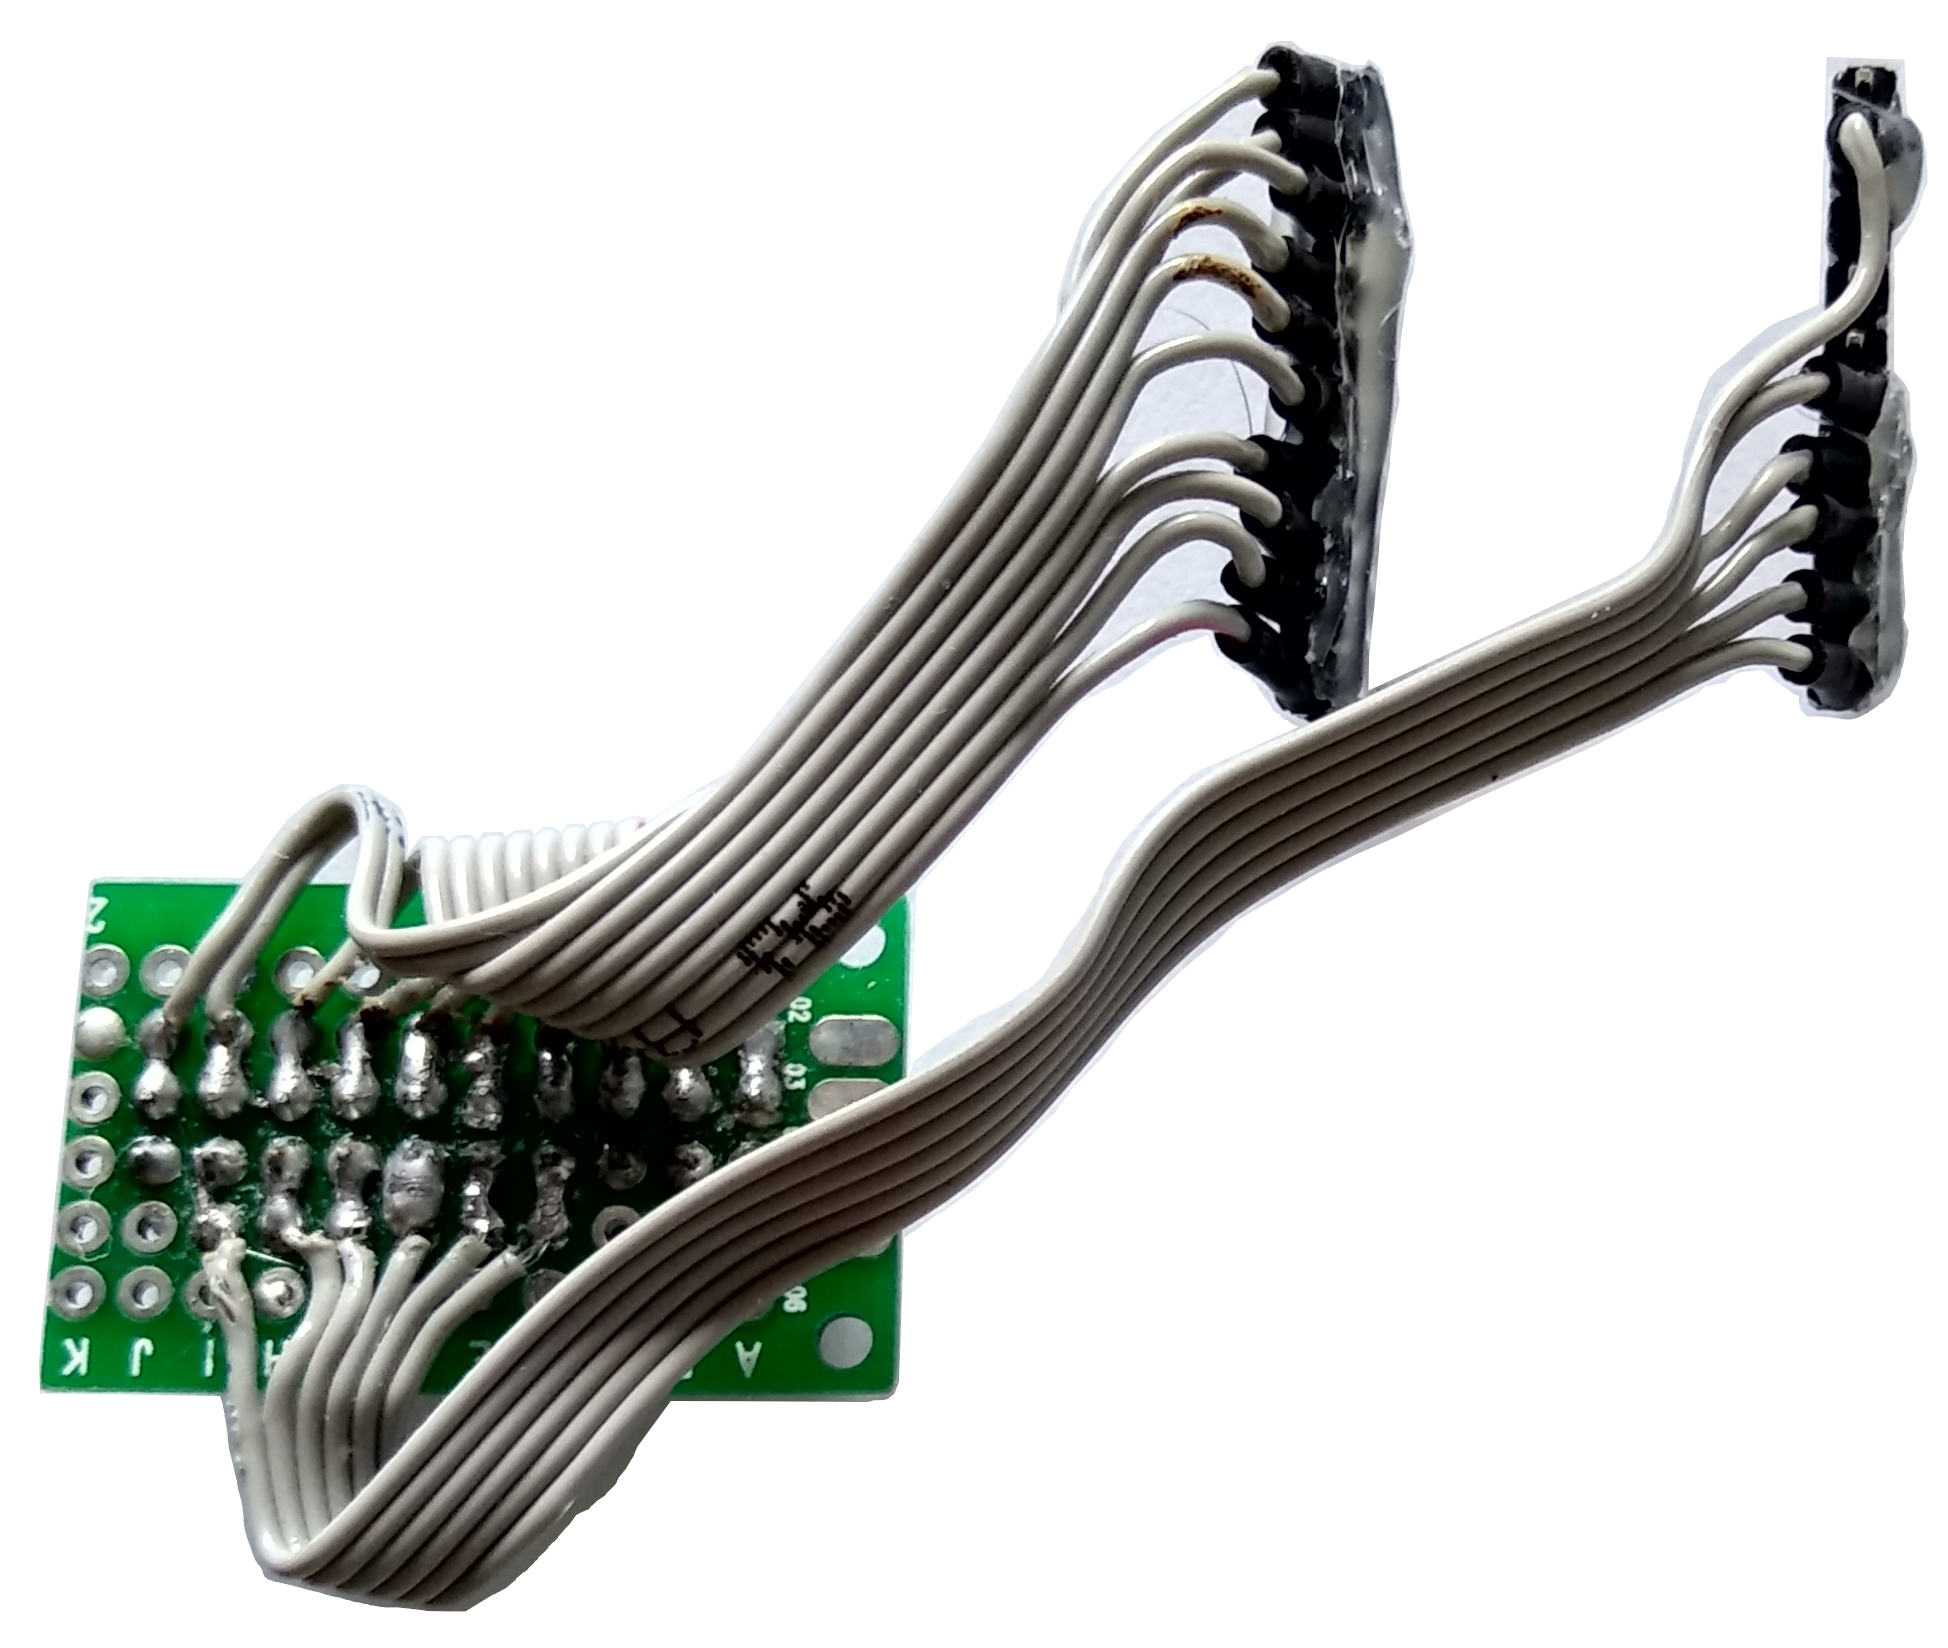
\includegraphics[height=40mm]{hw_final/cables_cut.jpg}
            \label{fig:matriz-hw-resto:cables}
        }
        \subfigure[Botones auxiliares]{
            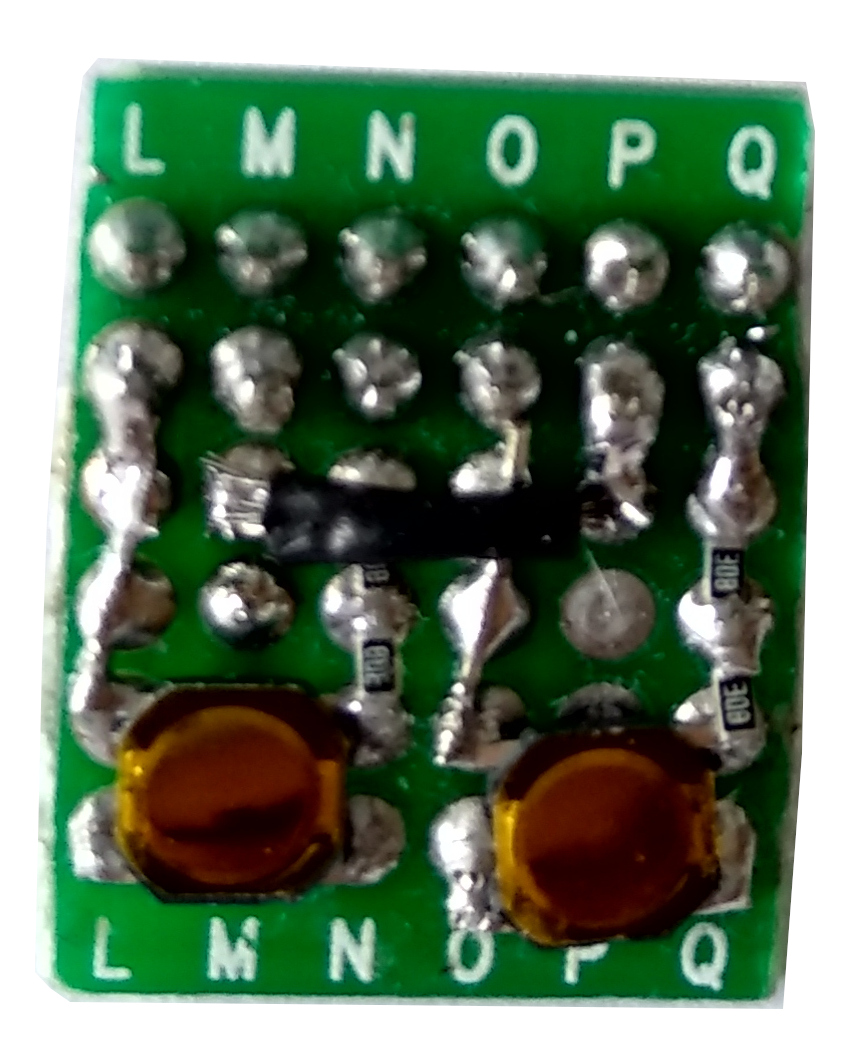
\includegraphics[height=40mm]{hw_final/buttons_cut.jpg}
            \label{fig:matriz-hw-resto:botones}
        } \\
        \subfigure[Base 3D]{
            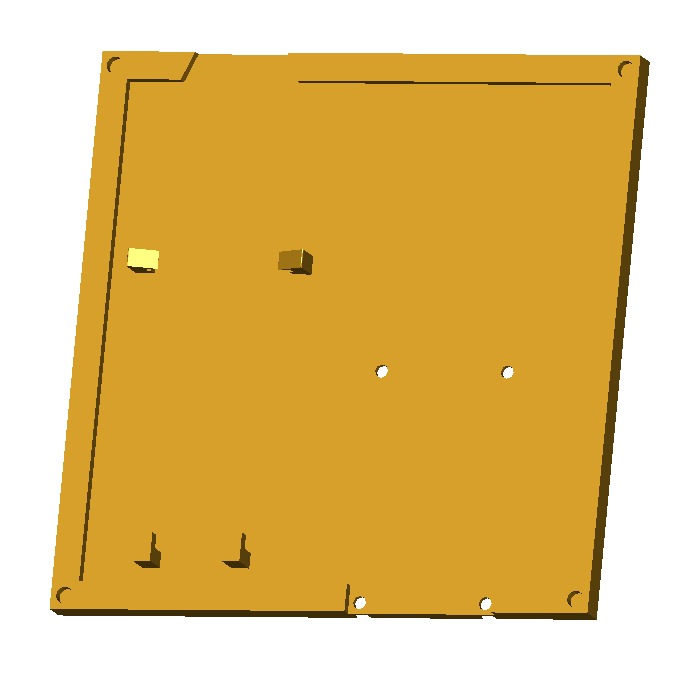
\includegraphics[height=75mm]{hw_final/3D_base.jpg}
            \label{fig:matriz-hw-resto:base}
        }
        \caption{Resto de elementos usados en el sistema de captación} 
        \label{fig:matriz-hw-resto}
    \end{figure}
\end{enumerate}

%!
\subsection{Módulos integrados en la FPGA.}
Siguiendo los objetivos planteados en el capitulo~\ref{ch:objetivos}, se han diseñado e implementado los siguientes módulos en la FPGA, todos en lenguaje Verilog.

\textbf{Nota.} En el anexo~\ref{ch:diagramas} se muestran de forma gráfica todas las relaciones existente entre ellos, mientras que en el anexo~\ref{ch:maquinas-estados} se plasman sus maquinas de estados \emph{Mealy} internas.

%* Comprobar
\subsubsection{Módulo divisor de reloj (clk\_div).}
Módulo que divide un reloj de entrada, tal que la frecuencia de salida sea $f_{out} = \frac{f_{in}}{2^n}$, donde $n$ es el número de \emph{Flip-Flops} tipo D utilizados, como se aprecia en la figura~\ref{fig:clk_div_esquema}. En el listado~\ref{src:resultados-modulos-clk-div} se plasman los parámetros, entradas y salidas del módulo.

\begin{figure}[hbt]
    \centering
    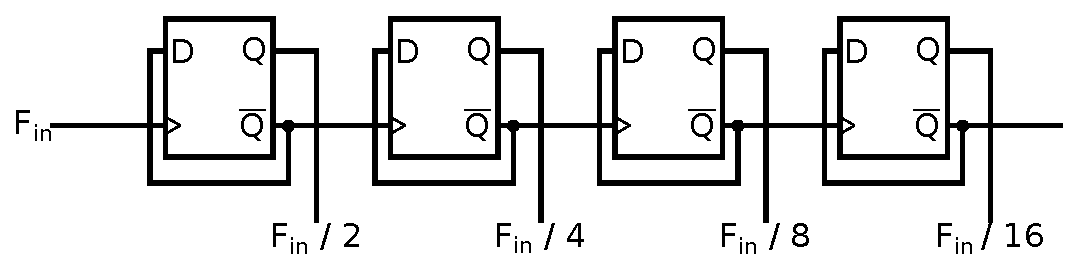
\includegraphics[width = 90mm]{esquemas/divisor_flipflop_D.eps}
    \caption{Divisor de reloj con \emph{Flip-Flops}}
    \label{fig:clk_div_esquema}
\end{figure}

A partir de él se generan dos relojes, uno basado en el reloj de $12MHz$ procedente de la placa \emph{iCEstick} (señal llamada clk\_div\_ice) y otro a partir del reloj de $60MHz$ del módulo USB3300 (señal  llamada clk\_div\_ULPI). Ambos relojes se dividen 24 veces y su única funcionalidad es la de  comprobar el funcionamiento del sistema por medio de los LEDs integrados en la placa.

\begin{lstlisting}[language=Verilog,
    caption={Parámetros, entradas y salidas del módulo clk\_div.},
    label=src:resultados-modulos-clk-div]
/*
 *
 * Módulo clk_div
 *
 * Parámetros:
 *  - DIVIDER. Número de veces que el reloj de referencia es dividido. f_clk_out = f_clk_in / (2^DIVIDER)
 *
 * Entradas:
 *  - enable. Cuando esta señal esté a nivel alto, el módulo estará activo, y en caso contrario la salida estará siempre a nivel bajo.
 *  - clk_in. Reloj de referencia a partir del cual se genera el de salida.
 *
 * Salidas:
 *  - clk_out. Señal de reloj generada con la frecuencia deseada.
 *  - clk_pulse. Señal con la misma frecuencia que el reloj de salida, pero con un ancho de pulso igual al del reloj de entrada.
 *
 */
\end{lstlisting}

% Parámetros:
% \begin{itemize}
%     \item \textbf{DIVIDER.} Número de veces que el reloj de referencia es dividido.
% \end{itemize}

% Entradas:
% \begin{itemize}
%     \item \textbf{enable.} Cuando esta señal esté a nivel alto, el módulo estará activo, en caso contrario, la salida estará siempre a valor bajo.
%     \item \textbf{clk\_in.} Reloj de referencia a partir del cual se genera el de salida.
% \end{itemize}

% Salidas:
% \begin{itemize}
%     \item \textbf{clk\_out.} Señal de reloj generada con la frecuencia deseada.
%     \item \textbf{clk\_pulse.} Señal con la misma frecuencia que el reloj de salida, pero con un ancho de pulso igual al del reloj de entrada.
% \end{itemize}


%* Comprobar
\subsubsection{Módulo de generación de reloj de baudios (clk\_baud\_pulse).}
De igual manera que el módulo divisor de reloj, este también genera uno, pero en esta ocasión en vez de utilizar directamente \emph{Flip-Flops}, se utiliza un contador, lo que permite una mayor precisión en la salida, con un ancho de pulso igual al del reloj de entrada. En el listado~\ref{src:resultados-modulos-clk-baud-pulse} se plasman los parámetros, entradas y salidas del módulo.

Este reloj generado, configurable por medio de un parámetro de entrada, es usado para controlar la velocidad (baudios) de lectura/escrituro en el módulo de comunicación serie, comentado más adelante.

\begin{lstlisting}[language=Verilog,
    caption={Parámetros, entradas y salidas del módulo clk\_baud\_pulse.},
    label=src:resultados-modulos-clk-baud-pulse]
/*
 *
 * Módulo clk_baud_pulse
 *
 * Parámetros:
 *  - COUNTER_VAL. Valor optimo a contar para generar el pulso deseado.
 *  - PULSE_DELAY. Numero de retrasos en la señal de salida antes producir un pulso.
 *
 * Entradas:
 *  - enable. Cuando esta señal esté a nivel alto, el módulo estará activo, y en caso contrario la salida estará siempre a nivel bajo, reiniciando además sus registros internos.
 *  - clk_in. Reloj de referencia a partir del cual se genera el de salida.
 *
 * Salidas:
 *  - clk_pulse. Pulso generado.
 *
 */
\end{lstlisting}


%* Comprobar
\subsubsection{Módulo de memoria FIFO (FIFO\_BRAM\_SYNC).}
Módulo que de forma sincrona en lectura y escritura al reloj, es capaz de almacenar datos en los bloques de RAM internos de la FPGA, de tal manera que el primer dato en ser introducido sea el primero en ser extraído. En el listado~\ref{src:resultados-modulos-fifo} se plasman los parámetros, entradas y salidas del módulo.

Se han creado dos variantes, FIFO\_BRAM\_SYNC y FIFO\_BRAM\_SYNC\_CUSTOM, ambas parten de la misma base de funcionamiento, pero la segunda permite utilizar más de un único bloque de RAM interna.

\begin{lstlisting}[language=Verilog,
    caption={Parámetros, entradas y salidas del módulo FIFO\_BRAM\_SYNC\_CUSTOM.},
    label=src:resultados-modulos-fifo]
/*
 *
 * Módulo FIFO_BRAM_SYNC_CUSTOM
 *
 * Parámetros:
 *  - ALMOST_FULL. Porcentaje mínimo de la memoria que hace que se active la señal wr_almost_full. Por defecto vale 0.9.
 *  - ALMOST_EMPTY. Porcentaje máximo de la memoria que hace que se active la señal rd_almost_empty. Por defecto vale 0.1.
 *  - DATA_WIDTH. Tamaño de cada valor almacenado. Por defecto vale 8bits.
 *  - FIFO_SIZE_ML. Número de bloques de RAM a usar. Por defecto se utiliza uno.
 *
 * Entradas:
 *  - rst. Señal de reinicio, activa a nivel bajo.
 *  - clk. Reloj de referencia.
 *  - wr_dv. Señal que indica que los datos de entrada deben ser almacenados.
 *  - wr_DATA. Datos a ser almacenados. Debe tener el mismo ancho que el parámetro DATA_WIDTH.
 *  - rd_en. Señal que indica que se desea leer los datos almacenados.
 *
 * Salidas:
 *  - wr_full. Señal que indica que la memoria esta llena. Futuras operaciones de escritura serán ignoradas.
 *  - wr_almost_full. Señal que indica que la memoria esta casi llena.
 *  - rd_DATA. Datos leidos de la memoria.
 *  - rd_empty. Señal que indica que la memoria esta vacía. Futuras operaciones de lectura serán ignoradas.
 *  - rd_almost_empty. Señal que indica que la memoria esta casi vacía.
 *
 */
\end{lstlisting}

% Parámetros:
% \begin{itemize}
    %     \item \textbf{\emph{ALMOST\_FULL}.} Porcentaje mínimo de la memoria que hace que se active la señal wr\_almost\_full. Por defecto vale $0.9$.
    %     \item \textbf{\emph{ALMOST\_EMPTY}.} Porcentaje máximo de la memoria que hace que se active la señal rd\_almost\_empty. Por defecto vale $0.1$.
    %     \item \textbf{\emph{DATA\_WIDTH}.} Tamaño de cada valor almacenado. Por defecto vale $8~bits$.
% \end{itemize}
% Entradas. Señales sincrona al flanco de subida del reloj.:
% \begin{itemize}
    %     \item \textbf{\emph{rst}.} Señal de reinicio, activa a nivel bajo.
%     \item \textbf{\emph{clk}.} Reloj de referencia.
%     \item \textbf{\emph{wr\_dv}.} Señal que indica que los datos de entrada deben ser almacenados. 
%     \item \textbf{\emph{wr\_DATA}.} Datos a ser almacenados. Debe tener el mismo ancho que el parámetro \emph{DATA\_WIDTH}.
%     \item \textbf{\emph{rd\_en}.} Señal que indica que se desea leer los datos almacenados.
% \end{itemize}
% Salidas:
% \begin{itemize}
%     \item \textbf{\emph{wr\_full}.} Señal que indica que la memoria esta llena. Futuras operaciones de escritura serán ignoradas.
%     \item \textbf{\emph{wr\_almost\_full}.} Señal que indica que la memoria esta casi llena.
%     \item \textbf{\emph{rd\_DATA}.} Datos leidos de la memoria.
%     \item \textbf{\emph{rd\_empty}.} Señal que indica que la memoria esta vacía. Futuras operaciones de lectura serán ignoradas.
%     \item \textbf{\emph{rd\_almost\_empty}.} Señal que indica que la memoria esta casi vacia.
% \end{itemize}


%* Comprobar
\subsubsection{Módulo de registro de desplazamiento universal (shift\_register).}
Submódulo capaz de desplazar tanto a izquierda como a derecha la información almacenada, y que a su vez, permita una carga y lectura en paralelo. En el listado~\ref{src:resultados-modulos-shift} se plasman los parámetros, entradas y salidas del módulo.

La finalidad de este submódulo es poder convertir datos de serie a paralelo o de paralelo a serie, cuando ocurra una recepción o transmisión respectivamente.

En la figura~\ref{fig:shift_esquema} se muestra, mostrando sus señales, el funcionamiento del registro de desplazamiento diseñado, en está ocasión, con desplazamiento hacia la derecha.

\begin{figure}[htb]
    \centering
    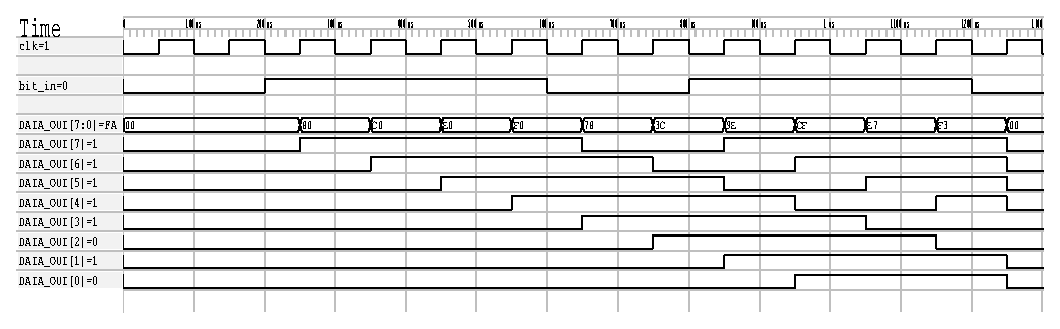
\includegraphics[height=46mm]{esquemas/shift_register.eps}
    \caption{Ejemplo de funcionamiento del registro de desplazamiento hacia la derecha.}
    \label{fig:shift_esquema}
\end{figure}

\begin{lstlisting}[language=Verilog,
    caption={Parámetros, entradas y salidas del módulo shift\_register.},
    label=src:resultados-modulos-shift]
/*
 *
 * Módulo shift_register
 *
 * Parámetros:
 *  - BITS. Tamaño en bits del registro de desplazamiento. El tamaño total será de BITS + 1 (bit de salida).
 *
 * Entradas:
 *  - clk. Reloj de referencia. Todas las operaciones se ejecutarán en el flanqueo de subida.
 *  - rst. Señal de reinicio, activa a nivel bajo.
 *  - bit_in. Bit a ser desplazado dentro del registro (modos 01 y 10).
 *  - DATA_IN. Datos a ser cargados de forma paralela (modo 11).
 *  - mode. Selector de operación a realizar [2 bits].
 *     > 00. No hacer nada.
 *     > 01. Desplazamiento a izquierda.
 *     > 10. Desplazamiento a derecha.
 *     > 11. Carga paralela.
 *
 * Salidas:
 *  - bit_out. Bit de salida tras el desplazamiento (modos 01 y 10).
 *  - DATA. Datos paralelos almacenados.
 *
 */
\end{lstlisting}


%* Comprobar
\subsubsection{Módulo de comunicación serie (UART).}
Sistema capaz de generar y recibir señales compatibles con una comunicación bidireccional serie 8N1\footnote{8N1: $8~bits$ de datos, sin $bit$ de paridad y un $bit$ de parada}, consiguiendo una tasa de transferencia estable máxima de $3750000~bauds$. Además, tanto para la lectura coma para la escritura, se han incorporado unos \emph{buffers} basados en memorias FIFO de $512~bytes$ cada uno. En el listado~\ref{src:resultados-modulos-uart} se plasman los parámetros, entradas y salidas del módulo.

Este módulo se ha dividido a su vez en los siguientes submódulos.
\begin{itemize}
    %* Comprobar
    \item \textbf{Submódulo de recepción serie (UART\_Rx).} \\
    Está continuamente esperando a que la señal de entrada de datos serie pase de un nivel alto a otro bajo, y una vez detectada esa caída, empezar a almacenar los $bits$ que conforman la trama a la velocidad dictada por el reloj de baudios. En la figura~\ref{fig:flujo_uart_rx} se muestra su flujo de funcionamiento.

    \begin{figure}[!hbt]
        \centering
        \scalebox{0.85} {\begin{tikzpicture}[auto]
    % Config
    \tikzFlow

    % Place nodes
    \node [flowStart] (idle) {Reposo};
    
    \node [flowDecision] at ($ (idle)+(0,-2.65) $) (rxLow) {Entrada del puerto serie a nivel bajo?};
    
    \node [flowBase, below of=rxLow] (init) {Reinicio del contador de $bits$};
    
    \node [flowBase] at ($ (rxLow.east)+(3.85,1) $) (read) {Se guarda $bit$ entrante en el registro de desplazamiento};

    \node [flowDecision, below of=read] (10bitsDone) {Se han leído los $10~bits$ del mensaje?};
    
    \node [flowBase] at ($ (read)+(4.1,0) $) (increase) {Incremento del contador de $bits$};

    \node [flowBase] at ($ (10bitsDone)+(4.1,0) $) (wait) {Se espera un pulso del reloj de baudios};

    \node [flowBase, below of=10bitsDone] (save) {Se almacena el byte en memoria};

    % % Draw edges
    \path [flowLine] (idle) -- (rxLow);
    \path [flowLine] (rxLow) -- (init);
    \path [flowLine] (init.south) |- +(3.5,-1) |- (read.west);
    \path [flowLine] (read) -- (10bitsDone);
    \path [flowLine] (increase) -- (read);
    
    \node [flowHide] at ($ (idle)+(2.75,0) $) (anchor1) {};
    \path [flowLine] (rxLow) -- node [right, xshift=-1.2cm] {Sí} (init);
    \path [flowLine] (rxLow.east) node [above, xshift=0.2cm] {No} -| (anchor1.center);
    
    \path [flowLine] (save.east) -| +(4.5,0) |- (idle.east);
    
    \path [flowLine] (wait) -- (increase);
    \path [flowLine] (10bitsDone.east) node [above, xshift=0.2cm] {No} -- (wait);
    \path [flowLine] (10bitsDone) -- node [right, xshift=-1.2cm] {Sí} (save);
\end{tikzpicture}


% \begin{tikzpicture}[auto]
%     % Config
%     \tikzFlow

%     % Place nodes
%     \node [flowStart] (idle) {Reposo};
    
%     \node [flowDecision, below of=idle] (rxLow) {Entrada del puerto serie a nivel bajo?};
    
%     \node [flowBase, below of=rxLow] (init) {Reinicio del contador de $bits$};
    
%     \node [flowBase, below of=init] (read) {Se guarda $bit$ entrante en el registro de desplazamiento};

%     \node [flowDecision, below of=read] (10bitsDone) {Se han leído los $10~bits$ del mensaje?};
    
%     \node [flowBase] at ($ (read)+(4.1,0) $) (increase) {Incremento del contador de $bits$};

%     \node [flowBase] at ($ (10bitsDone)+(4.1,0) $) (wait) {Se espera un pulso del reloj de baudios};

%     \node [flowBase, below of=10bitsDone] (save) {Se almacena el byte en memoria};

%     % % Draw edges
%     \path [flowLine] (idle) -- (rxLow);
%     \path [flowLine] (rxLow) -- (init);
%     \path [flowLine] (init) -- (read);
%     \path [flowLine] (read) -- (10bitsDone);
%     \path [flowLine] (increase) -- (read);
    
%     \node [flowHide] at ($ (idle)+(3.5,0) $) (anchor1) {};
%     \path [flowLine] (rxLow) -- node [right, xshift=-1.2cm] {Sí} (init);
%     \path [flowLine] (rxLow.east) -| node [above, xshift=-1.2cm] {No} (anchor1.center);
    
%     \path [flowLine] (save.east) -| +(4.5,0) |- (idle.east);
    
%     \path [flowLine] (wait) -- (increase);
%     \path [flowLine] (10bitsDone.east) node [above, xshift=0.2cm] {No} -- (wait);
%     \path [flowLine] (10bitsDone) -- node [right, xshift=-1.2cm] {Sí} (save);
% \end{tikzpicture}}
        \caption{Diagrama de funcionamiento del submódulo de recepción serie}
        \label{fig:flujo_uart_rx}
    \end{figure}
    
    %* Comprobar
    \item \textbf{Submódulo de emisión serie (UART\_Tx).} \\
    En este caso, cuando internamente se quiera enviar un mensaje, se exportan sucesivamente los $10bits$ que conforman la trama a la velocidad dada por el reloj de baudios. En la figura~\ref{fig:flujo_uart_tx} se muestra su flujo de funcionamiento.
    \begin{figure}[!hbt]
        \centering
        \scalebox{0.85} {\begin{tikzpicture}[auto]
    % Config
    \tikzFlow

    % Place nodes
    \node [flowStart] (idle) {Reposo};
    
    \node [flowDecision, below of=idle] (newData) {Existen datos a enviar?};

    \node [flowBase, below of=newData] (reset) {Reinicio del contador de $bits$};
    
    \node [flowStart, below of=reset] (load) {Carga de datos a enviar en el registro de desplazamiento};
    
    \node [flowStart, below of=load] (sendBit) {Se envía un bit, y se desplaza el registro};
    
    \node [flowDecision, below of=sendBit] (done) {Se han enviado los 10 bits del mensaje?};
    
    \node [flowBase] at ($ (done)+(4.2,0) $) (wait) {Se espera un pulso del reloj de baudios};

    \node [flowBase] at ($ (sendBit)+(4.2,0) $) (increase) {Incremento del contador de $bits$ enviados};

    % Draw edges
    \path [flowLine] (idle) -- (newData);
    \path [flowLine] (reset) -- (load);
    \path [flowLine] (load) -- (sendBit);
    \path [flowLine] (sendBit) -- (done);

    \node [flowHide] at ($ (idle)+(3.5,0) $) (anchor1) {};
    \path [flowLine] (newData.east) -| node [above, xshift=-1.2cm] {No} (anchor1.center);
    \path [flowLine] (newData) -- node [right, xshift=-1.2cm] {Sí} (reset);
    
    \path [flowLine] (wait) -- (increase);
    \path [flowLine] (increase) -- (sendBit);
    
    \path [flowLine] (done.south) node [right, xshift=-1.2cm, yshift=-0.3cm] {Sí} |- +(6.6,-1) |- (idle.east);
    \path [flowLine] (done.east) -- node [above, xshift=0cm] {No} (wait.west);
\end{tikzpicture}}
        \caption{Diagrama de funcionamiento del submódulo de emisión serie}
        \label{fig:flujo_uart_tx}
    \end{figure}
\end{itemize}

\newpage %!
\begin{lstlisting}[language=Verilog,
    caption={Parámetros, entradas y salidas del módulo UART.},
    label=src:resultados-modulos-uart]
/*
 *
 * Módulo UART
 *
 * Parámetros:
 *  - BAUDS. Valor optimo a contar para generar los baudios deseado.
 *
 * Entradas:
 *  - rst. Señal de reinicio, activa a nivel bajo.
 *  - clk. Reloj de referencia.
 *  - Rx. Datos serializados de de entrada.
 *  - I_DATA. Señal de 8bits que contiene los datos a ser enviados.
 *  - send_data. Señal que inicializa una transmisión de datos.
 *  - NxT. Señal para extraer un byte de datos del buffer de lectura.
 *
 * Salidas:
 *  - Tx. Datos serializados de de salida.
 *  - clk_Rx. Reloj, a la velocidad fijada por BAUDS, usado para recibir los datos.
 *  - clk_Tx. Reloj, a la velocidad fijada por BAUDS, usado para transmitir los datos.
 *  - O_DATA. Señal de 8bits que contiene los datos recibidos.
 *  - TiP. Señal que indcia que hay una transmisión en proceso.
 *  - NrD. Señal que indica la llegada de nuevos datos. Esta estará activa un pulso de clk.
 *  - Tx_FULL. Señal que indica que el buffer de transmisión interno está lleno.
 *  - Rx_FULL. Señal que indica que el buffer de recepción interno está lleno.
 *  - Rx_EMPTY. Señal que indica que el buffer de recepción interno está vacío.
 *
 */
\end{lstlisting}


%! Figuras
\subsubsection{Módulo de comunicación ULPI.}
Sistema, que de forma síncrona al reloj de $60MHz$ generado por el integrado \emph{USB3300}, es capaz tanto de procesar como de generar señales ULPI, tal como se contempla en su especificación\cite{ulpi-specs}. En el listado~\ref{src:resultados-modulos-ulpi} se plasman los parámetros, entradas y salidas del módulo.

De todos los modos de funcionamiento de dicho bus, y tal como se ha comentado en el capitulo \ref{ch:objetivos} de objetivos, se han creado unicamente submódulos encargados de leer y escribir registros, y el modo de recibir datos USB.

% \newpage %!
\begin{lstlisting}[language=Verilog,
    caption={Entradas y salidas del módulo ULPI.},
    label=src:resultados-modulos-ulpi]
/*
 *
 * Módulo ULPI
 *
 * Entradas:
 *  - rst. Señal de reinicio, activa a nivel bajo.
 *  - clk_ice. Reloj interno iCEstick de 12MHz.
 *  - clk_ULPI. Reloj externo de 60MHz.
 *  - PrW. Señal que activa la escritura de registro.
 *  - PrR. Señal que activa la lectura de registro.
 *  - ADDR. Dirección de 6bits que indica donde se van a escribir/leer los datos.
 *  - REG_VAL_W. Valor a ser escrito en el registro ULPI.
 *  - DATA_re. Señal que extrae un byte de los datos de captura.
 *  - INFO_re. Señal que extrae un paquete con la información de la ultima captura.
 *  - DIR. Señal del bus ULPI (DIRection).
 *  - NXT. Señal del bus ULPI (NeXT).
 *  - DATA_in. Señal de datos de entrada del bus ULPI.
 *
 * Salidas:
 *  - status. Señal que indica en que estado se encuentra el módulo (lectura, escritura, etc..)
 *  - busy. Señal que indica que el módulo está ocupado.
 *  - REG_VAL_R. Valor del registro leído.
 *  - RxCMD. Señal que contiene información relevante del bus USB.
 *  - RxLineState. Información del bus USB almacenada en RxCMD.
 *  - RxVbusState. Información del bus USB almacenada en RxCMD.
 *  - RxActive. Información del bus USB almacenada en RxCMD.
 *  - RxError. Información del bus USB almacenada en RxCMD.
 *  - RxHostDisconnect. Información del bus USB almacenada en RxCMD.
 *  - RxID. Información del bus USB almacenada en RxCMD.
 *  - USB_DATA. Datos capturados USB.
 *  - USB_INFO_DATA. Información de la última captura USB (RxCMD y tamaño).
 *  - DATA_buff_full. Señal que indica que el buffer de captura está lleno.
 *  - DATA_buff_empty. Señal que indica que el buffer de captura está vacio.
 *  - INFO_buff_full. Señal que indica que el buffer de información está lleno.
 *  - INFO_buff_empty. Señal que indica que el buffer de información está vacio.
 *  - DATA_out. Señal de datos de salida del bus ULPI.
 *  - STP. Señal del bus ULPI (SToP).
 *  - U_RST. Señal de reinicio del integrado USB3300.
 *
 */
\end{lstlisting}

En la siguiente lista se nombran los diversos submódulo que lo forman, inicializados posteriormente todos ellos en un mismo archivo, siguiendo el diagrama mostrado en la figura~\ref{fig:flujo_ulpi_main}.

\begin{figure}[!hbt]
    \centering
    \scalebox{0.8} {\begin{tikzpicture}[auto]
    % Config
    \tikzFlow

    % Place nodes
    \node [flowStart] (start) {Inicio};
    
    \node [flowDecision, below of=start] (init) {El integrado USB3300 ha inicializado el bus ULPI?};

    \node [flowBase, below of=init] (idle) {Reposo};
    
    \node [flowDecision, below of=idle] (recv) {El módulo de recepción USB está ocupado?};
    
    \node [flowDecision] at ($ (recv)+(-4,-2.5) $) (PrW) {Se quiere escribir un registro?};
    
    \node [flowDecision, below of=PrW] (PrR) {Se quiere leer un registro?};
    
    \node [flowBase] at ($ (PrW)+(9,0) $) (writeWait) {Esperar a finalización de escritura de registro (señal dada por ULPI\_REG\_WRITE)};

    \node [flowBase] at ($ (PrR)+(9,0) $) (readWait) {Esperar a finalización de lectura de registro (señal dada por ULPI\_REG\_READ)};

    \node [flowBase] at ($ (recv)+(5,0) $) (recvWait) {Esperar a finalización de captura USB (señal dada por ULPI\_RECV)};
    
    % Draw edges
    \path [flowLine] (start) -- (init);
    
    \path [flowLine] (init.east) node [above, xshift=0.35cm] {No} -| +(1,0) |- (start.east);
    \path [flowLine] (init) -- node [right, xshift=-1.1cm] {Sí} (idle);
    
    \path [flowLine] (idle) -- (recv);
    
    \path [flowLine] (recv.west) node [above, xshift=-0.35cm] {No} -| (PrW.north);
    \path [flowLine] (recv.east) node [above, xshift=0.35cm] {Sí} -- (recvWait);

    \path [flowLine] (PrW.east) node [above, xshift=0.35cm] {Sí} -- (writeWait.west);
    \path [flowLine] (PrW.south) -- node [right, xshift=-1.1cm] {No} (PrR.north);

    \path [flowLine] (PrR.east) node [above, xshift=0.35cm] {Sí} -- (readWait.west);
    \path [flowLine] (PrR.west) node [above, xshift=-0.35cm] {No} -| +(-1,0) |- (idle.west);

    \node [flowHide] at ($ (recvWait.east)+(1,0) $) (anchor1) {};
    \node [flowHide] at ($ (writeWait.east)+(1,0) $) (anchor2) {};
    \path [flowLine] (readWait.east) -| +(1,0) |- (idle.east);
    \path [flowLine] (writeWait.east) -- (anchor2.center);
    \path [flowLine] (recvWait.east) -- (anchor1.center);
\end{tikzpicture}}
    \caption{Diagrama de funcionamiento de la unión de módulos ULPI}
    \label{fig:flujo_ulpi_main}
\end{figure}

\begin{itemize}
    %* Comprobar
    \item \textbf{Submódulo de escritura de registros (ULPI\_REG\_WRITE).} \\
    Dándole una dirección de $6bits$ y un $byte$ de datos, este módulo genera las señales necesarias para la escritura de registros. En la figura~\ref{fig:flujo_ulpi_write} se muestra su flujo de funcionamiento.
    \begin{figure}[!hbt]
        \centering
        \scalebox{0.8} {\begin{tikzpicture}[auto]
    % Config
    \tikzFlow

    % Place nodes
    \node [flowStart] (idle) {Reposo};
    
    \node [flowDecision] at ($ (idle)+(-3,-2) $) (writeData) {Se desea escribir un registro?};
    
    \node [flowBase, below of=writeData] (init) {Preparación de dirección y datos};
    
    \node [flowBase, below of=init] (TxD) {Envío de TxD CMD de escritura};
    
    \node [flowDecision, below of=TxD] (NXTon1) {Señal NXT activa?};
    
    \node [flowBase] at ($ (idle)+(3,-2) $) (DATA) {Envío de los datos a almacenar};
    
    \node [flowDecision, below of=DATA] (NXTon2) {Señal NXT activa?};
    
    \node [flowBase, below of=NXTon2] (stop) {Activación de la señal de parada};
    
    \node [flowBase, below of=stop] (reset) {Reinicio de las variables de control};


    % Draw edges
    \path [flowLine] (idle) -| (writeData.north);
    \path [flowLine] (init) -- (TxD);
    \path [flowLine] (TxD) -- (NXTon1);
    
    \node [flowHide] at ($ (idle)+(0,1) $) (anchor1) {};
    \path [flowLine] (writeData) -- node [right, xshift=-1.2cm] {Sí} (init);
    \path [flowLine] (writeData.west) -- +(-0.5,0) |- node [right, xshift=-1.1cm, yshift=-1.2cm] {No} (anchor1.center);
    
    \node [flowHide] at ($ (NXTon1)+(0,1.2) $) (anchor2) {};
    \path [flowLine] (NXTon1.east) node [above, xshift=0.75cm] {Sí} -| +(1.5, 0) |- (DATA);
    \path [flowLine] (NXTon1.west) -- +(-0.5,0) |- node [left, xshift=1.75cm, yshift=-0.55cm] {No} (anchor2.center);

    \path [flowLine] (DATA) -- (NXTon2);
    \path [flowLine] (stop) -- (reset);
    
    \node [flowHide] at ($ (NXTon2)+(0,1.2) $) (anchor3) {};
    \path [flowLine] (NXTon2) -- node [right, xshift=-1.2cm] {Sí} (stop);
    \path [flowLine] (NXTon2.west) -- +(-0.5,0) |- node [right, xshift=-1.1cm, yshift=-0.7cm] {No} (anchor3.center);

    \path [flowLine] (reset.east) -| +(1,0) |- ($ (idle)+(0,1) $) -- (idle.north);
\end{tikzpicture}}
        \caption{Diagrama de funcionamiento del submódulo de escritura de registros ULPI}
        \label{fig:flujo_ulpi_write}
    \end{figure}
    
    %* Comprobar
    \item \textbf{Submódulo de lectura de registros (ULPI\_REG\_READ).} \\
    Dándole en esta ocasión únicamente la dirección de $6bits$, este genera las señales necesarias para que el integrado \emph{USB3300} envíe el valor del registro solicitado, valor que debe ser leído por este modulo. En la figura~\ref{fig:flujo_ulpi_read} se muestra su flujo de funcionamiento.
    \begin{figure}[!hbt]
        \centering
        \scalebox{0.8} {\begin{tikzpicture}[auto]
    % Config
    \tikzFlow

    % Place nodes
    \node [flowStart] (idle) {Reposo};
    
    \node [flowDecision] at ($ (idle)+(-3,-3) $) (readData) {Se desea leer un registro?};
    
    \node [flowBase, below of=readData] (init) {Preparación de dirección};
    
    \node [flowBase, below of=init] (TxD) {Envío del TxCMD de lectura};
    
    \node [flowDecision, below of=TxD] (NXTon) {Señal NXT activa?};
    
    \node [flowBase] at ($ (idle)+(3,-2) $) (wait1) {Primer ciclo de espera};
    
    \node [flowBase, below of=wait1] (DATA) {Lectura de datos};
    
    \node [flowBase, below of=DATA] (wait2) {Segundo ciclo de espera};   
    
    \node [flowBase, below of=wait2] (save) {Almacenaje del dato leído};

    \node [flowBase, below of=save] (reset) {Reinicio de las variables de control};


    % Draw edges
    \path [flowLine] (idle) -| (readData.north);
    \path [flowLine] (init) -- (TxD);
    \path [flowLine] (TxD) -- (NXTon);
    
    \node [flowHide] at ($ (idle)+(0,1) $) (anchor1) {};
    \path [flowLine] (readData) -- node [right, xshift=-1.2cm] {Sí} (init);
    \path [flowLine] (readData.west) -- +(-0.5,0) |- node [right, xshift=-1.1cm, yshift=-1.2cm] {No} (anchor1.center);
    
    \node [flowHide] at ($ (NXTon)+(0,1.2) $) (anchor2) {};
    \path [flowLine] (NXTon.east) node [above, xshift=0.75cm] {Sí} -| +(1.5, 0) |- (wait1);
    \path [flowLine] (NXTon.west) -- +(-0.5,0) |- node [left, xshift=1.75cm, yshift=-0.55cm] {No} (anchor2.center);

    \path [flowLine] (wait1) -- (DATA);
    \path [flowLine] (DATA) -- (wait2);
    \path [flowLine] (wait2) -- (save);
    \path [flowLine] (save) -- (reset);

    \path [flowLine] (reset.east) -| +(1,0) |- ($ (idle)+(0,1) $) -- (idle.north);
\end{tikzpicture}}
        \caption{Diagrama de funcionamiento del submódulo de lectura de registros ULPI}
        \label{fig:flujo_ulpi_read}
    \end{figure}
    
    %* Comprobar
    \item \textbf{Submódulo de obtención de datos USB (ULPI\_RECV).} \\
    Cada vez que el integrado \emph{USB3300} quiera enviar una captura de datos, pone a nivel alto la señal DIR y empieza a transmitir los datos. Este módulo está continuamente esperando dicho cambio, a partir del cual obtiene, clasifica y almacena los datos entrantes. En la figura~\ref{fig:flujo_ulpi_recv} se muestra su flujo de funcionamiento.
    \begin{figure}[!hbt]
        \centering
        \scalebox{0.8} {\begin{tikzpicture}[auto]
    % Config
    \tikzFlow

    % Place nodes
    \node [flowStart] (idle) {Reposo};
    
    \node [flowDecision, below of=idle] (allow) {Se está usando algún otro módulo ULPI?};

    \node [flowDecision, below of=allow] (DIR1) {DIR y NXT están a nivel alto?};
    
    \node [flowBase] at ($ (DIR1)+(-4,0) $) (init) {Inicio del contador de $bytes$};
    
    \node [flowDecision, below of=DIR1] (DIR2) {DIR sigue a nivel alto?};
    
    \node [flowBase] at ($ (DIR2)+(4.1,0) $) (save) {Almacenar en memoria TxdCMD y el numero de $bytes$ leídos};

    \node [flowBase, below of=DIR2] (read) {Leer datos ULPI};

    \node [flowDecision, below of=read] (NXT) {NXT está a nivel alto?};
    
    \node [flowBase] at ($ (NXT)+(-4,-2) $) (saveTxcmd) {Actualizar valor interno de TxdCMD con el valor leido};

    \node [flowBase] at ($ (NXT)+(4,-2) $) (saveByte) {Guardar en la memoria de datos USB el valor leido};

    \node [flowBase, below of=saveByte] (increase) {Incrementar contador de $bytes$};

    \node [flowBase] at ($ (DIR2)+(-4,0) $) (wait) {Esperar a siguiente ciclo};
    
    % Draw edges
    \path [flowLine] (idle) -- (allow);
    
    \node [flowHide] at ($ (allow.east)+(1,0) $) (anchor1) {};
    \path [flowLine] (allow.east) node [above, xshift=0.35cm] {Sí} -- (anchor1.center);
    \path [flowLine] (allow) -- node [right, xshift=-1.1cm] {No} (DIR1);
    \path [flowLine] (save.north) |- (anchor1.center);
    
    \path [flowLine] (DIR1.east) node [above, xshift=0.35cm] {No} -| +(1,0) |- (idle.east);
    \path [flowLine] (DIR1.west) node [above, xshift=-0.2cm] {Sí} -- (init);

    \path [flowLine] (DIR2.east) node [above, xshift=0.2cm] {No} -- (save.west);
    \path [flowLine] (DIR2) node [right, xshift=-1.1cm, yshift=-1.1cm] {Sí} -- (read);
    
    \path [flowLine] (init) -- (wait);
    \path [flowLine] (read) -- (NXT);
    
    \path [flowLine] (NXT.east) node [above, xshift=0.35cm] {Sí} -| (saveByte.north);
    \path [flowLine] (NXT.west) node [above, xshift=-0.35cm] {No} -| (saveTxcmd.north);
    
    \path [flowLine] (saveByte) -- (increase);
    
    \path [flowLine] (wait.east) -- (DIR2.west);

    \node [flowHide] at ($ (increase)+(-4,0) $) (anchor3) {};
    \path [flowLine] (increase.west) -| +(-9,0) |- (wait.west);
    \path [flowLine] (saveTxcmd.east) -| (anchor3.center);
\end{tikzpicture}}
        \caption{Diagrama de funcionamiento del submódulo de recepción USB}
        \label{fig:flujo_ulpi_recv}
    \end{figure}
\end{itemize}


%* Comprobar
\subsubsection{Módulo de procesado y almacenaje de comandos entrantes (ULPI\_op).}
Se ha diseñado e implementado un simple protocolo, con el que ser capaz de recibir las ordenes del sistema y de enviar los datos capturados.

Siempre que se desee ejecutar un comando en el sistema de captura, el PC envía $2~bytes$ (\emph{YYZZZZZZ\_XXXXXXXX}), separados a su vez en tres grupos, de 2, 6 y 8 $bits$ respectivamente. Tal como se recoge en la tabla~\ref{tab:comandos_operacion}, el primer grupo indica que comando se debe realizar, el segundo la dirección en la que realizar dicha operación, y el tercero, los datos a utilizar.

\begin{table}[htbp]
    \caption{Información de los $bytes$ enviados a la \emph{FPGA}.}
    \centering
    \label{tab:comandos_operacion}
    \begin{tabular}{|c|c|c|c|c|}
        \hline
        % Bits operación ($2~bits$) & Bits dirección ($6~bits$) & Bits datos ($8~bits$) & Descripción                                    & Respuesta \\ \hline
        Bits comando & Bits dirección & Bits datos & Descripción & Respuesta \\ \hline
        \hline
        00 & Indiferente & 10010110 & \begin{tabular}{@{}c@{}}Activar/desactivar \\ envío de datos USB\end{tabular} & --       \\ \hline
        01 & Indiferente & Indiferente & \begin{tabular}{@{}c@{}}Enviar último valor \\ de registro leído\end{tabular} & 1 byte   \\ \hline
        10 & Dirección a escribir & Datos a escribir & Escribir registro \emph{ULPI} & -- \\ \hline
        11 & Dirección a leer & Indiferente & Leer registro \emph{ULPI} & --              \\ \hline
    \end{tabular}
\end{table}

Estos $bytes$, tras ser recibidos por el módulo de comunicación serie, son recogidos por este módulo, el cual los clasifica y almacena hasta su ejecución.

\begin{lstlisting}[language=Verilog,
    caption={Entradas y salidas del módulo ULPI\_op.},
    label=src:resultados-modulos-ulpi-op]
/*
 *
 * Módulo ULPI_op
 *
 * Entradas:
 *  - rst. Señal de reinicio, activa a nivel bajo.
 *  - clk. Reloj de referencia.
 *  - UART_DATA. Datos del puerto serie.
 *  - UART_Rx_EMPTY. Señal que indica que el puerto serie no tiene datos disponibles.
 *  - op_stack_pull. Señal que indica que se quiere obtner un nuevo valor del buffer de operaciones.
 *
 * Salidas:
 *  - UART_NxT. Señal usada para obtener, si fuera posible, un nuevo byte.
 *  - op_stack_msg. Comando completo recibido y almacendao.
 *  - op_stack_full. Señal que indica que el buffer de operaciones está lleno.
 *  - op_stack_empty. Señal que indica que el buffer de operaciones está vacio.
 *
 */
\end{lstlisting}


%* Comprobar
\subsubsection{Módulos de control de botonera (btn\_debouncer y signal\_trigger).}
Al haber introducido varios botones externos, estos sufren una propiedad física de rebote, por la que el botón, al ser pulsado, salta entre varios estados antes de estabilizarse, produciendo pulsaciones no deseadas. Para solucionarlo, se ha creado un simple módulo que concatena varios \emph{Flip-Flops} tal como se muestra en la figura~\ref{fig:esquema-debounce}.

\begin{figure}[htb]
    \centering
    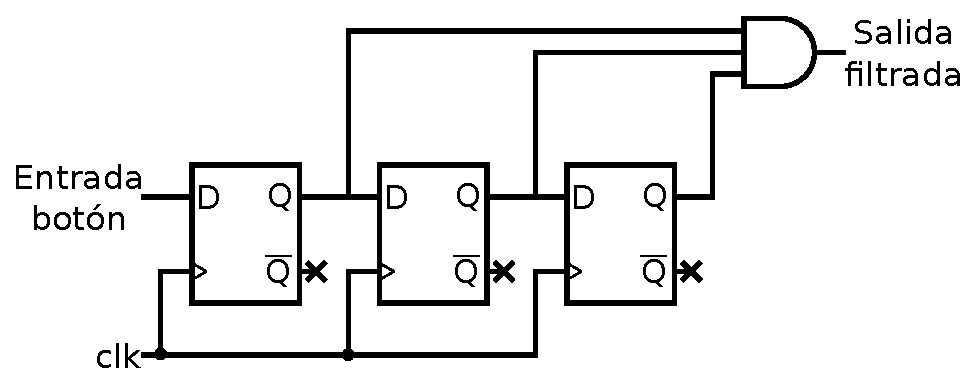
\includegraphics[width=80mm]{esquemas/debounce.eps}
    \caption{Esquema de funcionamiento del módulo btn\_debouncer}
    \label{fig:esquema-debounce}
\end{figure}

Por otro lado, como las pulsaciones del usario tienen una duración mucho mayor a la de un ciclo del reloj de control, se ha creado un segundo módulo que ante la pulsación de larga duración, envia un unico pulso con el mismo ancho que el del reloj de entrada.


%!
\subsubsection{Módulo de control maestro (main\_controller).}
Para el correcto funcionamiento del sistema, todos los módulos deben trabajar de forma coordiana, sin interferirse mutuamente. Por eso, se ha implementado este módulo, que 

Los modulos anteriormente explicados, no poseen relacion entre ellos, por tanto necesitan un módulo extra encargado de temporizar y distribuir que tareas deben realizar.

\begin{figure}[!hbt]
    \centering
    \scalebox{0.8} {\begin{tikzpicture}[auto]
    % Config
    \tikzFlow

    % Place nodes
    \node [flowStart] (idle) {Reposo};

    \node [flowDecision] at ($ (idle)+(5,-3) $) (newMsg) {Ha llegado un nuevo comando?};

    \node [flowDecision, below of=newMsg] (msgToggle) {El comando es de activación de envío de datos?};

    \node [flowDecision, below of=msgToggle] (msgSend) {El comando es de envío valor leído?};

    \node [flowDecision, below of=msgSend] (msgWrite) {El comando es de escritura de registro?};
    
    \node [flowDecision, below of=msgWrite] (msgRead) {El comando es de lectura de registro?};

    \node [flowDecision] at ($ (idle)+(0,-3) $) (newUSB) {Hay datos USB disponibles para enviar al PC?};


    \node [flowDecision] at ($ (idle)+(-5,-3) $) (push) {Se ha pulsado el botón de prueba?};
    \node [flowBase, below of=push] (testByte) {Envío de un $byte$ de prueba};





    % \node [flowStart] (idle) {Reposo};
    
    % \node [flowDecision, below of=idle] (rxLow) {Entrada del puerto serie a nivel bajo?};
    
    % \node [flowBase, below of=rxLow] (init) {Reinicio del contador de $bits$};
    
    % \node [flowBase, below of=init] (read) {Se guarda $bit$ entrante en el registro de desplazamiento};

    % \node [flowDecision, below of=read] (10bitsDone) {Se han leído los $10~bits$ del mensaje?};
    
    % \node [flowBase] at ($ (read)+(4.1,0) $) (increase) {Incremento del contador de $bits$};

    % \node [flowBase] at ($ (10bitsDone)+(4.1,0) $) (wait) {Se espera un pulso del reloj de baudios};

    % \node [flowBase, below of=10bitsDone] (save) {Se almacena el byte en memoria};

    % % % Draw edges
    % \path [flowLine] (idle) -- (rxLow);
    % \path [flowLine] (rxLow) -- (init);
    % \path [flowLine] (init) -- (read);
    % \path [flowLine] (read) -- (10bitsDone);
    % \path [flowLine] (increase) -- (read);
    
    % \node [flowHide] at ($ (idle)+(3.5,0) $) (anchor1) {};
    % \path [flowLine] (rxLow) -- node [right, xshift=-1.2cm] {Sí} (init);
    % \path [flowLine] (rxLow.east) -| node [above, xshift=-1.2cm] {No} (anchor1.center);
    
    % \path [flowLine] (save.east) -| +(4.5,0) |- (idle.east);
    
    % \path [flowLine] (wait) -- (increase);
    % \path [flowLine] (10bitsDone.east) node [above, xshift=0.2cm] {No} -- (wait);
    % \path [flowLine] (10bitsDone) -- node [right, xshift=-1.2cm] {Sí} (save);
\end{tikzpicture}}
    \caption{Diagrama de funcionamiento del módulo de control maestro}
    \label{fig:flujo_main_controller}
\end{figure}

%!
\subsection{Simulaciones finales.}
Con el objetivo de eliminar posibles errores capaces de dañar los propios componentes \emph{hardware}, y para comprobar el correcto funcionamiento del sistema, se han realizado diversas pruebas previas al sintetizado y utilización de la configuración final.

\begin{enumerate}
    %! Revisar
    \item \textbf{Pruebas de botones auxiliares.}
    Se simulan las pulsaciones de los botones externos de la \emph{FPGA}, produciendo un reinicio con el primero, y un envío de un $byte$ por el puerto serie con el segundo.

    %! Revisar
    \item \textbf{Prueba de lectura de registro.}
    Se simula una petición enviada por el puerto serie, que realice una lectura de registro \emph{ULPI}.
    
    %! Revisar
    \item \textbf{Prueba de transmisión del último registro leído.}
    Se simula una petición enviada por el puerto serie para enviar el valor del registro anteriormente leído al PC.
    
    %! Revisar
    \item \textbf{Prueba de escritura de registro.}
    Se simula una petición enviada por el puerto serie, que escriba un $byte$ en un registro del integrado \emph{USB3300}.
    
    %! Revisar
    \item \textbf{Prueba de captación de 6 bytes USB.}{\label{enum:captacion_6}}
    Prueba en la que se simula la llegada de $6~bytes$ de datos USB, se comprueba también el correcto guardado de los mismos en la memoria interna de la \emph{FPGA}.
    
    %! Revisar
    \item \textbf{Prueba de activación de la transmisión de datos capturados.}{\label{enum:activacion_transmision}}
    Se simula una petición enviada por el puerto serie, con la que activar el envío automático de los datos capturados.
    
    %! Revisar
    \item \textbf{Prueba de captación de 4 bytes USB.}
    De igual manera que la prueba \ref{enum:captacion_6}, pero enviando esta vez $4~bytes$ con el envio de datos al PC activado.
    
    %! Revisar
    \item \textbf{Prueba de captación de cambios de estado del bus USB.}
    Se simula un cambio de estado USB enviado por el bus \emph{ULPI}, observando si se actualiza en la \emph{FPGA}.
    
    %! Revisar
    \item \textbf{Prueba de finalización de la transmisión de datos capturados.}
    De igual manera que en la prueba \ref{enum:activacion_transmision} se activaba el envió de datos automático, se realiza la misma petición, desactivandolo en este caso.
\end{enumerate}


%!
\subsection{Información del sintetizado final.}




%!
\section{Resultados del \emph{software} de control y guardado.}
\noWord[Comentar más de esta frase, ya que la utilizo mas adelante] El sistema en su conjunto no sería funcional, sin una aplicación que utilice los recursos creados para recibir y almacenar la captura.



%! Revisar
\subsection{Aplicaciones de utilidad.}
% lenguaje, hilos, librerías, etc...
A medida que se ha ido desarrollando la parte \emph{hardware}, se han creado varias utilidades en lenguaje \emph{Python}, con las que realizar cálculos de forma rápida o con las que comprobar el funcionamiento de ciertas partes del sistema. Hay que destacar:
\begin{enumerate}
    %* Comprobar
    \item \textbf{Utilidad de divisiones del reloj.} \\
    Utilidad con la que poder realizar de forma rápida varios cálculos relacionados con los relojes de entrada. Por ejemplo, obtener los valores óptimos con los que dividir un reloj para generar unos baudios deseados. En el listado \ref{src:utilidad_divisiones_reloj_out}, se plasma un ejemplo de uso.
    \begin{lstlisting}[
        caption={Ejemplo de la utilidad de divisiones de reloj.},
        label=src:utilidad_divisiones_reloj_out]
$ ./get_divider.py
  Usage: ./get_divider.py [option] arg1 arg2
  Options: 
      -o: Print the optimal counter value for a given clock (arg1) and Serial baudrate (arg2). [Default]
      -b: Print the minimal divider value for a given clock (arg1) and Serial baudrate (arg2).
      -d: Print the minimal divider value for a given clock (arg1) and time (arg2).
      -t: Print the time (and serial baudrate) for a given clock (arg1) and divider (arg2).
      -a: Print, for a given clock (arg1), all the possible periods that can be generated between 0 and arg2.
      -c: Print the clock for a given time (arg1) and divider (arg2).
$ ./get_divider.py -o 12000000 115200
  Optimal counter value: 105
$ ./get_divider.py -b 12000000 9600
  Recomended divider (with 18% error): 10 [8.533333333333334e-05s]
  10 [8.533333333333334e-05s] - [0.00010416666666666667s] - 11 [0.00017066666666666668s]          
    \end{lstlisting}
    
    %! Revisar
    \item \textbf{Utilidad de generación de baudios.} \\
    Pequeña aplicación que, para los $baudios$ más comunes, genere varias definiciones de \emph{Verilog} a usar por el módulo encargado de generar el reloj de baudios. En el listado \ref{src:utilidad_baudios_out} se muestra un ejemplo de la salida de la aplicación.
%     \\ \noWord[Borrar listado??? La verdad, es algo inutil ponerlo]
%     \begin{lstlisting}[
%         caption={Ejemplo de la utilidad de generación de baudios ante \emph{60 MHz} de entrada.},
%         label=src:utilidad_baudios_out]
% $ ./gen_bauds.py
%   `define B921600 66
%   `define B460800 131
%   `define B256000 235
%   `define B230400 261
%   `define B153600 391
%   `define B128000 469
%   `define B115200 521
%   `define B57600  1042
%   `define B56000  1072
%   `define B38400  1563
%   `define B28800  2084
%   `define B19200  3125
%   `define B14400  4167
%   `define B9600   6250
%   `define B4800   12500
%   `define B2400   25000
%   `define B1200   50000
%   `define B600    100000
%   `define B300    200000
%   `define B110    545455
%     \end{lstlisting}
    
    %! Revisar
    \item \textbf{Utilidad de control serie.} \\
    Aplicación, que usando la librería encargada de controlar puertos serie, compruebe el funcionamiento del protocolo. Se puede configurar para abrir el puerto serie a cualquier velocidad, y poder enviar comandos de prueba.
\end{enumerate}

%!
\subsection{Información de la aplicación.}
Tal como se ha comentado al principio de esta sección, aun teniendo mayor carga la parte \emph{hardware}, es esencial implementar una aplicación que se comunique con la FPGA y permita su funcionamiento.

Para ello, utilizando lenguaje C, se ha creado una aplicación que dando opciones de control con una simple interfaz, es capaz de enviar comandos o recibir datos USB, y a su vez, es capaz de almacenarlos para su posterior uso o estudio.

La aplicación se ha dividido de la siguiente manera:
\begin{enumerate}
    %!
    \item \textbf{Hilo encargado de controlar las entradas de usuario.} \\
    Tanto la configuración a usar para conectarse a la \emph{FPGA} (puerto serie y baudios), como los comandos a enviar, son introducidos al programa por medio de un simple menú.

    \begin{lstlisting}[
        caption={Ejemplo de la utilidad de generación de baudios ante \emph{60 MHz} de entrada.},
        label=src:utilidad_]
$ .sddf
    \end{lstlisting}
    
    %!
    \item \textbf{Hilo encargado de gestionar la comunicación con la \emph{FPGA}, así como almacenar la trama capturada.}
    Por un lado, este hilo envio los comandos introducidos por el usuario a la FPGA, y por otro, cuando llegen los datos USB capturados, estos son almacenados en un archivo.
\end{enumerate}


%!
\subsection{Información del archivo generado.}
% Info JSON, como interpretarlo, imagen de ejemplo, etc...
Se ha elegido almacenar la información captruada en un archivo formato JSON\footnote{INFO JSON}, 

\begin{lstlisting}[
    caption={Ejemplo de la utilidad de generación de baudios ante \emph{60 MHz} de entrada.},
    label=src:utilidad_]
$ .sddf
\end{lstlisting}


%!
\subsection{Conversión de JSON a PCAP.}
% Info JSON, como interpretarlo, imagen de ejemplo, etc...
Para poder analizar la captura en la aplicación \emph{Wireshark}, se ha creado otra utilidad, que a partir del archivo JSON generado anteriormente, lo transforma a PCAP.






% \chapter{Resultados}
% \label{ch:resultados-plantilla}

% Escribe en este capítulo los resultados del proyecto.  Este capítulo debería explicar los resultados de forma global, no los resultados de cada iteración.  Probablemente será el capítulo con más tablas y gráficas.  Revisa las secciones~\ref{sec:figuras} y~\ref{sec:tablas} para aprender cómo se escriben en \LaTeX{}. %! Revisar
\chapter{Discusión de resultados}
\label{ch:discusion-resultados}

La discusión de resultados se presenta de forma separada a los resultados propiamente dichos, porque de esta forma los resultados son directamente aprovechables en cualquier trabajo derivado.  Pero si el capítulo queda demasiado pequeño no dudes en mezclarlo con el anterior en un único capítulo de \emph{Resultados y discusión} o con el siguiente en un capítulo de \emph{Discusión de resultados y conclusiones}.



% \chapter{Discusión de resultados}
% \label{ch:discusion-resultados-plantilla}

% La discusión de resultados se presenta de forma separada a los resultados propiamente dichos, porque de esta forma los resultados son directamente aprovechables en cualquier trabajo derivado.  Pero si el capítulo queda demasiado pequeño no dudes en mezclarlo con el anterior en un único capítulo de \emph{Resultados y discusión} o con el siguiente en un capítulo de \emph{Discusión de resultados y conclusiones}. %!
\chapter{Conclusiones}
\label{ch:conclusiones}

%* Listo
En este capitulo se plasman las principales conclusiones del presente trabajo, y a su vez, se proponen posibles mejoras y trabajos futuros de interés.

%* Listo
\section{Conclusiones}
A continuación se detallan las principales conclusiones obtenidas durante la realización de este proyecto:

\begin{itemize}
    %* Listo
    \item Se ha procedido, en un primer lugar, a un análisis de mercado, confirmando la escasez de analizadores USB \emph{hardware} de bajo coste. Reafirmando de esa forma la finalidad del proyecto.
    
    %* Listo
    \item Se ha procedido a la selección y posterior conexión de los diversos componentes utilizados. Estos incluyen la placa de evaluación \emph{USB3300}, la placa de desarrollo \emph{iCEstick}, cableado de conexión, botonera y una base impresa en 3D.
    
    %* Listo
    \item Todo ello ha supuesto un precio de aproximadamente 45\$ (40\texteuro~al cambio), lo que supone una gran diferencia respecto a los analizadores comerciales, y una reducción de 43\$ respecto al proyecto de \emph{Ultra-Embedded} de similares características.
    
    %* Listo
    \item Se ha establecido una metodología de diseño y elaboración de módulos, que ha permitido una gran eficiencia en su elaboración, consiguiendo a su vez, una menor probabilidad de fallos y una alta reutilización.
    
    %* Listo
    \item El sistema soportar tramas USB 2.0 \emph{low speed}, \emph{full speed} y \emph{high speed}. Para esta última, debido a la escasa cantidad de memoria RAM disponible, puede haber perdida de datos si ocurre una gran transferencia USB en un breve periodo de tiempo.

    %* Listo
    \item Para el funcionamiento del sistema, se han diseñado y elaborado varios módulos, incluidos los establecidos en los objetivos, en el lenguaje descriptor de \emph{hardware} Verilog. \\
    Todos ellos han utilizado el 63\% de los bloques lógicos y el 100\% de los bloques de RAM disponibles en la FPGA usada. \\
    Principalmente hay que destacar los siguientes módulos.
    \begin{enumerate}
        \item Memoria FIFO.
        \item Registro de desplazamiento.
        \item Módulo de comunicación ULPI.
        \item Módulo de comunicación serie.
        \item Módulos generadores de relojes.
        \item Controlador maestro del sistema.
    \end{enumerate}

    %* Listo
    \item Se ha desarrollado una aplicación con las todas opciones necesarias para poder configurar la FPGA y recibir una captura, siendo esta almacenada en un archivo \emph{JSON} de fácil lectura.
    
    %* Listo
    \item Posteriormente, y para cumplir el objetivo propuesto, se ha creado una herramienta que convierte la trama capturada de formato \emph{JSON} a \emph{PCAP}.
    
    %* Listo
    \item Como observación final, hay que comentar varios aspectos a destacar en el uso de las FPGAs en general.
    \begin{itemize}
        \item Permiten una gran flexibilidad a la hora de realizar cualquier diseño de electrónica digital, y a diferencias de otros elementos como microcontroladores, permiten un alto nivel de paralelización de tareas, por lo que son de gran utilidad en ciertos diseños.
        
        \item Como contrapartida, las FPGAs introducen la necesidad de controlar las frecuencias máximas que pueden soportar, y una dificultad extra a la hora de realizar depuraciones.
    \end{itemize}
\end{itemize}

%* Listo
Con todo lo anteriormente expuesto, se puede afirmar que se han cumplido todos los objetivos establecidos al principio del trabajo, recogidos en el capítulo~\ref{ch:objetivos}.



%* Listo
\section{Trabajos futuros}
A continuación se enumeran varios trabajos futuros que se pueden realizar para mejorar el resultado del proyecto.

\begin{itemize}
    %* Listo
    \item Debido a la baja cantidad de memoria disponible en la FPGA usada, puede ser de gran interés añadir un módulo de memoria RAM externa, en la que almacenar de forma temporal los datos.
    
    %* Listo
    \item Implementación de un nuevo sistema de comunicación entre la FPGA y el PC, que prescindiendo del puerto serie actual, permita una mayor tasa de transferencia.
    
    %* Listo
    \item Diseño de una PCB que unifique los componentes utilizados en una sola placa, y se deshaga de todos aquellos innecesarios, como puede ser el emisor/receptor de infrarrojos de la placa iCEstick. Realizando esta tarea, a parte de obtener un producto más refinado, se puede disminuir aun más el precio final del sistema.
    
    %* Listo
    \item Creación de un disector para la utilidad de análisis \emph{Wireshark}, que sea capaz de mostrar más detalles de los datos capturados en el archivo \emph{PCAP}.
    
    %* Listo
    \item Introducción de herramientas de filtrado USB en la propia FPGA, que facilite el análisis. Por ejemplo, se podrían añadir filtros según el PID o la longitud de los datos a capturar.

    %* Listo
    \item Introducción de un sistema que permita saber en que instante temporal a ocurrido la captura de cada paquete de datos. Para ello, se puede añadir por ejemplo un circuito RTC (\emph{Real Time Clock}, o Reloj en Tiempo Real en español) que añada una marca temporal a cada paquete de datos obtenido.
\end{itemize}


% \chapter{Conclusiones}
% \label{ch:conclusiones-plantilla}

% Las conclusiones deben cerrar el documento, destacando los aspectos más importantes de la ejecución del TFG.  Debe analizar qué objetivos se han alcanzado y en qué grado, qué objetivos se han tenido que dejar fuera del proyecto y por qué, y qué líneas de trabajo futuro abre el TFG.  Para esta última parte es especialmente útil la lista \emph{Blocked} y la lista \emph{Backlog} de tu tablero Trello.

% En total las conclusiones no deberían superar dos o tres hojas.  Si ves que se alarga demasiado, traslada material al capítulo de discusión de resultados.

% Fíjate en que los objetivos abren el trabajo personal y las conclusiones lo cierran.  Procura mantener un orden que resalte esta relación. %* Comprobar


%! Manual de instalación y utilización
%! Yosys, nextpnr, icestorm tools, hacar compilacion, app, etc...

%!!
% Bib. USB in a nutshell
% Bib. USB specification
% Bib. Obijuan